% concatenated from type2paper.tex
\documentclass[a4paper, 11pt]{article}

\if0
\setlength{\topmargin}{0cm}
\setlength{\oddsidemargin}{0cm}
\setlength{\evensidemargin}{0cm}
\setlength{\textheight}{23truecm}
\setlength{\textwidth}{16truecm}
\fi


%\usepackage[dvipdfmx,usenames]{color}
%\usepackage[
%[dvipdfmx, 
%colorlinks,
%linkcolor=MidnightBlue,
%urlcolor=blue,
%bookmarksopenlevel=4
%]{hyperref}

%\usepackage{pxjahyper}

%\usepackage{xcolor}
\usepackage{ulem}
\usepackage{comment}
\usepackage{tikz-cd}

\usepackage{tikz}
\usepackage{amsmath, amssymb}
\usepackage{mathrsfs}
\usepackage{thm-restate}

%\usepackage{theorem}
\usepackage{amsthm}
\usepackage{color}
\usepackage{graphics}
\usepackage{mathtools}

\usepackage{xurl}


%\theorembodyfont{\rmfamily}      
%\theoremstyle{break}        

%\theoremstyle{definition}
\newtheorem{defn}{Definition}[section]  
\newtheorem{rem}[defn]{Remark} 
\newtheorem{exam}[defn]{Example}

\theoremstyle{plain}
\newtheorem{thm}[defn]{Theorem}
\newtheorem{theor}{Theorem}
\renewcommand{\thetheor}{\Alph{theor}}

\newtheorem{prop}[defn]{Proposition} 
\newtheorem{lem}[defn]{Lemma} 
\newtheorem{cor}[defn]{Collorary}

\newtheorem{thms}{Theorem} 
\newtheorem*{thm*}{Theorem}
\renewcommand{\thethms}{\thesection.\Alph{thms}}



\makeatletter


\makeatother


\newenvironment{pf}{\proof[Proof]}{\endproof}
\newenvironment{pf*}[1]{\proof[#1]}{\endproof}



\newcommand{\myclaim}{問題}
\newtheorem{claim}[defn]{\myclaim}

\newenvironment{myclm}[1]{%
  \renewcommand{\myclaim}{#1}\begin{claim}}{%
  \end{claim}\renewcommand{\myclaim}{問題}}


\newcommand{\?}{\textcolor{red}{??}}

\newcommand{\lm}{\lambda}
\newcommand{\llm}{{\lambda}'}
\newcommand{\Lm}{\Lambda}
\newcommand{\fp}{\mathbb{F}_p}
\newcommand{\fpp}{\mathbb{F}_{p^2}}
\newcommand{\fq}{\mathbb{F}_q}
\newcommand{\ocl}{\overline{C_{\lambda}}}
\newcommand{\ocll}{\overline{C_{{\lambda}'}}}
\newcommand{\oes}{\overline{E_s}}
\newcommand{\bA}{\mathbb{A}}
\newcommand{\bC}{\mathbb{C}}
\newcommand{\bP}{\mathbb{P}}
\newcommand{\bQ}{\mathbb{Q}}
\newcommand{\bN}{\mathbb{N}}
\newcommand{\bZ}{\mathbb{Z}}
\newcommand{\kb}{\overline{k}}

\newcommand{\F}{\mathbb{F}}
\newcommand{\Z}{\mathbb{Z}}
\newcommand{\N}{\mathbb{N}}
\newcommand{\cO}{\mathcal{O}}
\newcommand{\ord}{{\operatorname{ord}}}
\newcommand{\End}{{\operatorname{End}}}
\newcommand{\Aut}{{\operatorname{Aut}}}

\newcommand{\Asim}{\underset{\alpha}{\sim}}
\newcommand{\Bsim}{\underset{\beta}{\sim}}
\newcommand{\BBsim}{\underset{{\beta}'}{\sim}}
\newcommand{\Csim}{\underset{\gamma}{\sim}}
\newcommand{\piB}{{\pi}_{\beta}}
\newcommand{\piBB}{{\pi}_{{\beta}'}}
\newcommand{\piA}{{\pi}_{\alpha}}
\newcommand{\piC}{{\pi}_{\gamma}}
\newcommand{\super}{\text{supersingular}}

\newcommand{\height}{\operatorname{ht}}
\newcommand{\SL}{\operatorname{SL}}

\title{The Lang-Trotter conjecture on average for genus-$2$ curves with $S_3$ reduced automorphism group }
\author{Chihiro Ando\thanks{Graduate School of Environment and Information Sciences, Yokohama National University.
E-mail: \texttt{ando.chihiro.zs@gmail.com} } \  and Shushi Harashita\thanks{Graduate School of Environment and Information Sciences, Yokohama National University.
E-mail: \texttt{harasita@ynu.ac.jp}}}
\date{}

\begin{document}

\maketitle


\begin{abstract}
    \noindent 
    For an elliptic curve $E$ over $\mathbb{Q}$ without complex multiplication, Lang and Trotter conjectured that the number of primes $p <X$ at which $E$ has a supersingular reduction is asymptotically equal to $c\sqrt{X}/\log X$, where $c>0$ is a constant depending only on $E$. While it remains an open question, an average estimation related to the Lang--Trotter conjecture was established by Fouvry and Murty. This result is called the Lang--Trotter conjecture on average. We extend the Lang--Trotter conjecture to curves of genus $2$ and obtain a similar result to the Lang--Trotter conjecture on average for the family of curves $C_{\lambda}:y^2=x(x-1)(x-{\lambda})(x-(\lambda-1)/{\lambda})(x-1/ (1-\lambda))$. These curves are characterized as curves of genus $2$ with reduced automorphism group containing symmetric group $S_3$. 
    
\end{abstract}

\section{Introduction}
For an elliptic curve $E$ over $\mathbb{Q}$ with complex multiplication, Deuring proved that the number of primes $p <X$ at which $E$ has a supersingular reduction is asymptotically equal to 
 \[
 \frac{1}{2} \frac{X}{\log X}.
 \]
 For an elliptic curve $E$ over $\mathbb{Q}$ without complex multiplication, Lang and Trotter conjectured that the number of such primes is asymptotically equal to 
 \[\frac{c\sqrt{X}}{\log X},\]
 where $c>0$ is a constant depending only on $E$. It is still an open question, however,  Elkies \cite{Elkies} proved a weaker result, namely that there are infinitely many supersingular primes. Furthermore, an average estimation related to the Lang--Trotter conjecture was established by Fouvry and Murty \cite{FM01}.  They calculated 
 \begin{eqnarray*}
    && \frac{1}{AB} \sum_{\lvert a \rvert \le A} \sum_{\lvert b \rvert \le B}  \#\{p<X\mid E_{a,b} \textrm{ has a supersingular reduction at } p\}\\
    &&\sim \frac{4 \pi}{3} \frac{\sqrt{X}}{\log X},
 \end{eqnarray*}
for $A,B > X^{1+ \epsilon}$, where $E_{a,b}$ is an elliptic curve defined by an equation $y^2=x^2+ax+b$ and $a,b$ run through the integers. They also showed that the above average estimation holds for $A,B > X^{1/2+ \epsilon}$ and $AB > X^{3/2 +\epsilon}$. This result is called \textit{the Lang--Trotter conjecture on average}. One of the key \textcolor{black}{points} in their proof is that the number of supersingular elliptic curves $E_{a,b}$ over $\fp$ ($p \neq2,3$) with $0 \le a,b < p $ can be written as
\[
\frac{p}{2} \cdot \left(h(-4p)+h(-p) \right)+O(p),
\]
where $h(-p)$ and $h(-4p)$ are the class numbers of primitive quadratic forms with discriminants $-p$ and $-4p$, respectively. We note that $E_{a,b}$ has a supersingular reduction at $p$ if and only if the trace of the Frobenius morphism of $E_{a,b}/\fp$, denoted by $a_p(E_{a,b})$, is zero and that the result by Fouvry and Murty is the case of $a_p(E_{a,b})=0$. It was extended to the case $a_p(E_{a,b})=r$ for any $r\in \bZ$ by David and Pappalardi \cite{DP} and the improved result was given by Baier \cite{SB}. 

In this paper, we extend the Lang--Trotter conjecture on average to curves of genus 2. Let $K$ be an algebraically closed field of characteristic $p \ne 2$. Curves of genus $2$ are
classified into 7 types \textcolor{black}{with respect to their reduced automorphism groups (cf.\ Igusa \cite[\S\ 8]{Igusa}, also see \cite[1.2]{IKO02}). Here, the \textit{reduced automorphism group} ${\rm RA}(C)$ of hyperelliptic curve $C$ is the quotient of the automorphism group of $C$ by the central subgroup generated by the hyperelliptic involution.} 
In our previous work \cite{Ando}, we obtained the Lang--Trotter conjecture on average for the family of genus-$2$ curves
\[
y^2=x(x-1)(x+1)(x-{\lambda}) \left(x-\frac{1}{\lambda}\right),
\]
\textcolor{black}{whose reduced automorphism groups contain Klein-$4$ group}.
In the present paper, we focus on another type of them, the genus-$2$ curves defined by the following equation with parameter $\lm \in K$:
\[
C_{\lm}:y^2=x(x-1)(x-{\lambda}) \left(x-\frac{\lambda-1}{\lambda}\right)\left(x-\frac{1}{1-\lambda}\right).
\]
 These genus-$2$ curves are characterized as having the reduced automorphism group ${\rm RA}(C_\lambda)$ containing symmetric group $S_3$. For almost all $\lambda$, it is known that ${\rm RA}(C_\lambda)$ is isomorphic to $S_3$. 
Let $p$ be a prime such that $p \ge 5$. We consider whether $C_{\lm}$ has a superspecial reduction at $p$.
Here, a curve $C$ over a field $K$ is \textit{superspecial} if its Jacobian variety is isomorphic to a product of supersingular elliptic curves over $\overline{K}$, the algebraic closure. 
Our aim is to compute the average of 
\[
{\phi}_{\lm}(X):= \# \lbrace p<X \mid C_{\lm} \text{ has a superspecial reduction at } p  \rbrace .
\]
for $\lm\in \bQ$. To this end, we firstly determine the value 
\[
{\psi}_{p} := \# \lbrace \lm \in \fp \mid C_{\lm} \text{ is superspecial}  \rbrace 
\]
for each prime $p$. 
The number of isomorphism classes of superspecial genus-$2$ curves was computed for each of the 7 types by
Ibukiyama, Katsura and Oort \cite{IKO02}. In addition, the number of isomorphism classes of superspecial genus-$2$ curves that have models over $\fp$ was determined by Ibukiyama and Katsura \cite{IKadd} in terms of the class numbers and the type numbers. 
Moreover, Katsura and Oort \cite{KatsuraOort} obtained the number of $(a,b) \in {\overline{\fp}}^2$ 
such that the genus-$2$ curve $C_{a,b}:y^2=(x^2-1)(x^2-a)(x^2-b)$ is superspecial.
%and also counted superspecial $C_{a,b}$'s having reduced automorphism group containing $V_4$. 
However, neither the number of $(a,b) \in {\fp}^2$ such that the genus-2 curve $C_{a,b}$ is superspecial has not been argued, nor the number of $\lambda\in\fp$ such that $C_\lambda$ is superspecial.  The first theorem determines $\psi_p$ in terms of the class numbers $h(-p)$ and $ h(-3p)$. 
\begin{restatable}{theor}{thmA} \label{thm:A}
     Let $p\ge 5$ be a prime. Then we have 
    \begin{enumerate}
        \item [] ${\psi}_{p}=\frac{3}{2}h(-3p)$ if $p \bmod 4=1$,
        \item [] ${\psi}_{p}=0$ if  $p \bmod 12=7$,
        \item [] ${\psi}_{p}=3h(-p)$ if $p \bmod 12=11$.
    \end{enumerate}
\end{restatable}
To prove Theorem \ref{thm:A}, we use the result of Ibukiyama, Katsura and Oort \cite[\S 1.2]{IKO02} that $C_{\lm}$ is superspecial if and only if two elliptic curves 
 \begin{equation*}\label{eq:E_Lambda}
     E_{{\Lm}^{-}(\lm)}:y^2=x(x-1)\left(x-(1-\lambda)(\lm - \sqrt{{\lambda}^2-\lambda+1})^2 \right)
 \end{equation*}
 and 
\begin{equation*}\label{eq:E_LambdaPrime}
 E_{{\Lm}^{+}(\lm)}:y^2=x(x-1)\left(x-(1-\lambda)(\lm +\sqrt{{\lambda}^2-\lambda+1})^2 \right)
 \end{equation*}
 are supersingular. 
  Thus, it suffices to count the number of $\lambda \in \fp$ such that two associated elliptic curves $E_{\Lm^{-}(\lm)}$ and $ E_{{\Lm}^{+}(\lm)}$ are supersingular. \textcolor{black}{In fact, if either of the elliptic curves is supersingular, then both are supersingular (cf.\ \cite[Proposition 1.10]{IKO02}).  
To count such $\lm\in\fp$, a new and more elaborate argument was needed, as outlined below, because the defining equation contains radicals and differs from those treated in previous works (e.g. \cite{AT02}, \cite{Ando} and \cite{FM01}) on elliptic curves.}
 We firstly show that the $j$-invariants of supersingular elliptic curves $E_{\Lm^{-}(\lm)}$ and $ E_{{\Lm}^{+}(\lm)}$ are the roots of $P_{3p}(X) \bmod p$ if $p \equiv1 \bmod 4$ and are the roots of $P_{p}(X) \bmod p$ if $p \equiv3 \bmod 4$ and that conversely any root of $P_{3p}(X) \bmod p$ for $p \equiv1 \bmod4$ and any root of $P_{p}(X)\bmod p$ for $p \equiv3 \bmod 4$ is equal to the $j$-invariant of a supersingular elliptic curve $E_{\Lm^{\varepsilon}(\lm)}$ with some $\lm \in \fp$ and $\varepsilon\in\{\pm1\}$ (see Section \ref{the-important}). Here $P_{3p}(X)$ and $P_p(X)$ are the Hilbert class polynomials of level $3p$ and $p$ respectively (see \S \ref{complex}). An important fact is that the degrees of the polynomials $P_{3p}(X)$ and $P_p(X)$ are $h(-3p)$ and $h(-p)$ respectively.  We require an elaborate argument, since the endomorphism rings of the elliptic curves are far from obvious. 
 We also use the factorization of $P_{3p}(X)$ and $P_p(X)$ mod $p$ to 
 determine the value $\psi_p$. The factorization of $P_p(X) \bmod p$ for $p \equiv3\bmod4$ was determined by Elkies \cite{Elkies} or Kaneko \cite[Appendix]{kaneko} but that of $P_{3p}(X) \bmod p $ for $p\equiv1 \bmod 4$ has not been obtained, so we give a careful observation concerning $P_{3p}(X) \bmod p$ for $p \equiv1 \bmod 4$ in Section \ref{observationoffactorization}.

Using the value $\psi_p$, we compute the average of $\phi_{\lm}(X)$ for $\lm \in \bZ$ such that $|\lm|$ is less than a positive number $N>X^{1+\epsilon}$.
 \begin{restatable}{theor}{thmB}
 \label{thm:B}
    Let $X,\epsilon$ be positive numbers and $N$ a positive number that satisfies $N > X^{1+\epsilon}$. Then, we have
    \[
   \frac{1}{N} \sum_{\lvert \lm \rvert \le N} {\phi}_{\lm}(X) \sim \frac{(6+4\sqrt{3})\pi}{9} \frac{\sqrt{X}}{\log X} 
    \]
    as $X \rightarrow \infty$.
\end{restatable}
We use the idea of Fouvry and Murty, and this theorem is followed by a similar argument to our previous work \cite[\S 5]{Ando}.

Furthermore, we also calculate the average of $\phi_\lm(X)$ for $\lm\in \bQ$ such that $\height{(\lm)}<N$. Here, for $\lm=b/a$ with coprime numbers $a,b$, the height of $\lm$, denoted by $\height{(\lm)}$, is max$\{|a|,|b|\}$.
\begin{restatable}{theor}{thmC} \label{thm:C}
      Let $X,\epsilon$ be positive numbers and $N$ a positive number that satisfies $N > X^{1+\epsilon}$. Then,
    \[
   \frac{1}{N^2} \sum_{\lm \in \bQ,\ \height(\lm) \le N } {\phi}_{\lm}(X) \sim \frac{4(3+2\sqrt{3})}{3\pi} \frac{\sqrt{X}}{\log X} 
    \]
    as $X \rightarrow \infty$.
 \end{restatable}
 This result immediately follows from Theorem \ref{thm:B} and our previous work \cite[\S 6]{Ando}.

Our paper is organized into 10 sections. In Section \ref{preliminaries} we recall some properties of elliptic curves with complex multiplication in addition to the Hilbert class polynomials and the modular polynomials and related results by Gross-Zagier. We also review genus-$2$ curves. These are crucial in the proof of Theorem \ref{thm:A}.  Furthermore, we recall an analytic result that we use in the proof of Theorem B. In Section \ref{isogeniesbetweenElaElad}, we construct isogenies between the two elliptic curves $E_{\Lm^{-}(\lm)}$ and $E_{\Lm^{+}(\lm)}$ and in Section \ref{supersingularellwithlambda} we give details of the properties of supersingular elliptic curves $E_{\Lm^{\pm}(\lm)}$ with $\lm \in \fp$ and finally determine their endomorphism rings. In Section \ref{with Endomorphism containing}, we conversely observe elliptic curves over $\overline{\fp}$ with a certain endomorphism ring. In Section \ref{the-important} we discuss the relationship between the $j$-invariants of the supersingular elliptic curves $E_{\Lm^{\pm}(\lm)}$ and the Hilbert class polynomials. In Section \ref{observationoffactorization} we determine the factorization of $P_{3p}(X) \bmod p$ for $p \equiv1 \bmod 4$. We finally prove Theorem \ref{thm:A} in Section \ref{pfofa}, Theorem \ref{thm:B} in Section \ref{pfofb} and Theorem \ref{thm:C} in Section \ref{pfofc}. 

%\sout{In addition, the programs used in the computations appearing in the proof are
%available at the following GitHub repository:\\
%\url{https://github.com/tremolopluschihiro/Codes_for_the_LT_conjecture_on_average_for_genus2_curves_with_S3_reducedautomorphism_group}}

\subsection*{Acknowledgements}
This paper is a part of master’s thesis of the first author. She thanks
the second author for his supervision and for his helpful advice.  The authors also thank Toshiyuki Katsura for his helpful comments.
%The author also thanks Toshiyuki Katsura for his helpful comments.
%This research was supported by JSPS Grant-in-Aid for Scientific Research (C) 21K03159. 
 
\section{Preliminaries}
\label{preliminaries}
In this section, we recall some known results on
elliptic curves with complex multiplication as well as some properties of the Hilbert class polynomials and the modular polynomials and related results by Gross-Zagier. %\textcolor{red}{\sout{In addition, we}} 
We also review degree-$3$ isogenies of elliptic curves %\textcolor{red}{\sout{. Furthermore, we}, and} 
and recall some properties of genus-$2$ curves. Finally, we look at an analytic result for the Legendre symbol.

\subsection{The Hilbert class polynomials and modular polynomials }
\label{complex}
In this section, we recall the Hilbert class polynomials and modular polynomials.

Let $D$ be a positive integer with $D\equiv0,3 \bmod 4$ and consider an imaginary quadratic order of discriminant $-D$:
\[
O_D=\bZ\left[\frac{D+\sqrt{-D}}{2}\right].
\]
The Hilbert class polynomial of level $D$ is the monic polynomial $P_D(X)$ whose roots are precisely the distinct $j$-invariants of elliptic curves over $\overline{\bQ}$ with complex multiplication by $O_D$. It is well-known that the degree of $P_{D}(X)$ is equal to the class number of $O_D$ and that $P_{D}(X)$ has its coefficients in the ring of integers. Hence it makes sense to consider $P_D(X)$ mod prime $p$. Let $E$ be an elliptic curve and $p$ an odd prime such that $E$ has a good reduction at $p$. Next lemma explains when $E$ has a supersingular reduction at $p$.
\begin{lem}[Deuring:\cite{Deu}]
\label{nonquadraticp}
Let $p$ be an odd prime of good reduction for $E$. Then $E$ has supersinular redction at $p$ if and only if there exists some $D \equiv 0 \textrm{ or }3 \mod 4$ such that 
$p$ divides the numerator of $P_{D}(j(E))$ and $\left(\frac{-D}{p}\right)=-1$ or the highest power of $p$ dividing $D$ is odd. 
\end{lem}
Deuring also proved that complex multiplication in characteristic $p$ 
can be lifted to characteristic zero.

\begin{thm}[The Deuring lifting theorem]
\label{deuring}
    Let $A_0$ be an elliptic curve in characteristic $p$, with an endomorphism $\alpha_0$ which is not trivial. Then there exists an elliptic curve $A$ defined over a number field, an endomorphism $\alpha$ of A, and non-degenerate reduction of $A$ at a place $\mathfrak{B}$ lying above $p$, such that $A_0$ is isomorphic to $\overline{A}$, the reduction of $A$ at $\mathfrak{B}$, and $\alpha_0$ corresponds to $\overline{\alpha}$ under the isomorphism.  
\end{thm}
\begin{proof}
    S. Lang:\cite[Chapter 13, Theorem 14]{SL}
\end{proof}
 We examine the behavior of the Hilbert class polynomials mod $p$. Elkies obtained the factorization of $P_p(X) \bmod p$ as follows:

\begin{prop}[{Elkies:\cite{Elkies}}]
\label{fac_P_p}
Let $p$ be a prime with $p \equiv3 \bmod p$. Then the Hilbert class polynomial $P_p(X)$ factors into $(X-12^3)R(X)^2$ mod $p$ where $R(X)\in\fp[X]$ is a separable polynomial such that $R(12^3)\ne0 \bmod p$.
\end{prop}
Kaneko \cite[Appendix]{kaneko} gives another proof of this proposition using the Kronecker \textcolor{black}{relations (Propositions \ref{prop:kronecker1} and \ref{mojularandhirbert} below) on} the Hilbert class polynomials and the modular polynomials. Here, the modular polynomial $\Phi_n(X,Y)$ is a polynomial in $X$ and $Y$ characterized by
the condition that $\Phi_n(j(E_1),j(E_2))=0$
if and only if there exists an isogeny $E_1 \to E_2$
of elliptic curves whose kernel is a cyclic group of order $n$.

\begin{prop}[Lang:{\cite[5,\S2]{SL}}]
\label{prop:kronecker1}
    Let $p$ be a prime and $\Phi_p(X,Y)$  a modular polynomial. Then we have
    \[
    \Phi_p(X,j) \equiv(X-j^p)(X^p-j) \pmod p.
    \]
\end{prop}
There is a generalization of \textcolor{black}{this proposition.}
\begin{prop}
\label{generalkronecker}
    Let $p$ be a prime and $n$ an integer with $\gcd(n,p)=1$. Then we have
\[
\Phi_{pn}(X,j) \equiv \Phi_n(X,j^p)\Phi_n(X^p,j) \pmod p.
\]
\end{prop}
\begin{proof}
    Igusa \cite[p.569]{Igusa_ell} or Deuring \cite{Deu}. 
\end{proof}
We further recall the relation between the Hilbert class polynomials and the modular polynomials.  The next theorem tells us that the modular polynomials can be written as a product of the Hilbert class polynomials.
\begin{prop}[Lang:{\cite[10, Appendix]{SL}} ]
\label{mojularandhirbert}
Let $r(n,D)$ be the number of primitive $O_D$-equivalence classes of elements $\mu\in O_D$ such that $N(\mu)=n$. Here $\mu$ is called primitive if it does not lie in $nO_D$ for any positive integer $n\ne1$ and two elements of $O_D$ are said to be $O_D$-equivalent if their quotient is a unit in $O_D$. Then there exists a constant $c_n$ such that
\[
\Phi_n(X,X)=c_n \prod_{ D }P_D(X)^{r(n,D)}.\]

    %lang の本に載ってるやつ．モジュラー多項式との関係
\end{prop}

\subsection{Singular moduli by Gross-Zagier}\label{subsec:GZ}

Gross-Zagier \cite{GZ} computed a power of
the resultant of $P_{D_1}(X)$ and $P_{D_2}(X)$ for fundamental discriminants $-D_1,-D_2$ with $\gcd(D_1,D_2)=1$.
Let $w_i$ be the number of roots of unity
in $\cO_{D_i}$ for $i=1,2$ (Note $w_i=6$ for $D_i=3$ and $w_i=2$ for others).
They studied
\begin{equation}
J(-D_1,-D_2) = \prod_{E_1,E_2}(j(E_1)-j(E_2))^{\frac{4}{w_1w_2}},
\end{equation}
where $E_i$ runs over the isomorphism classes of elliptic curves \textcolor{black}{whose endomorphism ring is isomorphic to $\cO_{D_i}$.}  They showed that $J(-D_1,-D_2)^2$ is an integer and gave a formula for this integer,
which enables us to know its prime factorization.
Suppose that a prime $p$ is a divisor of $J(-D_1,-D_2)^2$.
Then it implies that there exists an $(E_1,E_2)$ such that the reductions  of $E_1$ and $E_2$ at some prime ideal $\frak p$ dividing $p$, considered over a number field,
are isomorphic to each other.

\begin{comment}
We discuss the case that
$(D_1,D_2) = (D,3p)$ where 
$-D$ and $-3p$ are fundamental with $\gcd(D,3p)=1$. 
%By Proposition \ref{Elkies-Kaneko}, the set of the roots of $P_{4p}(X)$ is the set of supersingular $j$-invariants belonging to $\F_p$.
%By the last remark in Section \ref{subsec:GZ}, $J(-D,-4p)^2$ should know the ``number" 
%of supersingular reductions defined over $\F_p$
%of elliptic curves with CM of type $D$.
%As we mentioned above, we discuss $J(-D,-4p)^2$ 
%for fundamental $-D$ and $p \equiv 1 \mod 4$ with $\gcd(D,4p)=1$.
Let $w$ be the number of roots of unity in $\cO_D$ (For fundamental $-D$, we have $w=6$ for $D=3$ and $w=2$ for others).
\end{comment}
This is a just application of Gross-Zagier \cite[Thm.\ 1.3 and Lem.\ 3.6]{GZ}, but we state a description of the weighted sum (by the cardinality of the automorphism groups over $\overline{\F}_p$) of the numbers of reductions modulo $p$ of elliptic curves with complex multiplication of type $D_i$ for $i=1,2$ with $\left(\frac{-D_1}{p}\right) = -1$ and $p|D_2$. Note
the $j$-invariants of the reductions belong to ${\F}_{p^2}$,
since they are supersingular.
% if $-D$ and $-4p$ are fundamental and coprime.
%with $\left(\frac{-D}{p}\right)=-1$, a question asks
%how many $E$ with CM of ${\mathcal O}_D$
%has a reduction over the prime field $\F_p$.
%The next theorem answers this question
%if $-D$ and $-4p$ are fundamental.
\begin{comment}
\begin{thm}[\textcolor{red}{To be checked}]\label{thm:GZ_for_3p}
Assume  that $-D$ is fundamental
and that $p \equiv 1 \pmod 4$ with $(D,3p) = 1$ and $\left(\frac{-D}{p}\right)\ne 1$. 
Then  
\begin{equation}\label{eq:GZ_for_3p}
\frac{1}{w}
\sum_{j}
%_{
%\begin{aligned}
%    [E]\text{\rm : CM of type }D\\
% j(E_p) \in \F_p
%\end{aligned}
% }
m_j\cdot \#\Aut(E_j)=    \ord_p J(-D, -3p)^2
\end{equation}
with the summation over distinct roots $j\in\F_{p^2}$ of the greatest common divisor of $P_D(X) \bmod p$ and $P_{3p}(X) \bmod p$, where $m_j$ is the product of the multiplicities at $j$ of $P_D(X) \bmod p$ and $P_{3p}(X) \bmod p$.
%the reduction of $E$ modulo $p$ and
%$E$ runs over the isomorphism classes of
%elliptic curves of CM type $D$ with $j(E_p)\in\F_p$.
\end{thm}
\end{comment}

\begin{thm}\label{thm:GZ_for_3p}
Assume  that $-D_1$ and $-D_2$ are fundamental and coprime with $\left(\frac{-D_1}{p}\right) = -1$ and $p|D_2$. 
Then  
\begin{equation}\label{eq:GZ_for_3p}
\frac{2}{w_1w_2}
\sum_{j}
%_{
%\begin{aligned}
%    [E]\text{\rm : CM of type }D\\
% j(E_p) \in \F_p
%\end{aligned}
% }
m_j\cdot \#\Aut(E_j)=    \ord_p J(-D_1, -D_2)^2
\end{equation}
with the summation over distinct roots $j\in\F_{p^2}$ of the greatest common divisor of $P_{D_1}(X) \bmod p$ and $P_{D_2}(X) \bmod p$, where $m_j$ is the product of the multiplicities at $j$ of $P_{D_1}(X) \bmod p$ and $P_{D_2}(X) \bmod p$.
%the reduction of $E$ modulo $p$ and
%$E$ runs over the isomorphism classes of
%elliptic curves of CM type $D$ with $j(E_p)\in\F_p$.
\end{thm}
\begin{proof}
Let $K={\mathbb Q}(\sqrt{-D_2})$.
Let $j$ be a root of $P_{D_2}(X)$. Note that $j$ belongs to the Hilbert class field $H$ of $K$. Let $\frak p$ be a finite place of $H$ lying over $p$
and $A$ the completion of the maximal unramified extension of the ring of $\frak p$-adic integers in $H$. In this case, $W:=A[w]$ for any $w$ which satisfies an integral quadratic equation of discriminant $-D_1$
is equal to $A$. Consider an element of $H$
\[
\alpha_j = \prod_{j_1}(j-j_1)^{\frac{4}{w_1w_2}},
\]
where  $j_1$ runs over all roots of $P_{D_1}(X)$.
Let $\pi$ be a uniformizer of $W$. Let $E_j$ denote an elliptic curve over $W$ of $j$-invariant $j$. 
By Gross-Zagier \cite[3.2]{GZ}, we have
\begin{equation}\label{eq:ord_alpha}
{\rm ord}_{\frak p}(\alpha_j) = \frac{4}{w_1w_2}\sum_{j_1}\sum_{n=1}^\infty \frac{1}{2}\# {\rm Iso}_{W/\pi^n}(E_j,E_{j_1}),
\end{equation}
where $j_1$ runs over all roots of $P_{D_1}(X)$ and ${\rm Iso}_{W/\pi^n}(E,E')$ is the set of isomorphisms from $E$ to $E'$ over $W/\pi^n$.
According to Dorman \cite[Theorem 3.13]{Dorman},  ${\rm Iso}_{W/\pi^n}(E_j,E_{j_1})$ is empty if $n\ge 2$. 
Hence, considering the sum of \eqref{eq:ord_alpha} over all roots $j$ of $P_{D_2}(X)$, we have the formula \eqref{eq:GZ_for_3p}.
%Put
%\[
%[\alpha,\beta] = \begin{pmatrix}\alpha & \beta\\ -q\overline{\beta} & %\overline{\alpha} \end{pmatrix}
%\]
%, the endomorphism ring
%\[
%{\rm End}_{W/\pi^n}(E) = \{\alpha,\beta]: ..., \beta\equiv 0 \bmod %{\frak p}^n\}
%\]
\end{proof}

Here we write the formula of Gross-Zagier:
\[
\ord_p J(-D_1, -D_2)^2 = 
\sum_{\begin{split}
    x\in\Z \text{ s.t.\;} x^2 < D_1D_2\\
    x^2\equiv D_1D_2 \bmod 4
\end{split}}
\ord_p F\left(\frac{D_1D_2-x^2}{4}\right)
\]
%\[
%\ord_p J(-D, -4p)^2 = \sum_{\begin{aligned}
%    x\in\Z \text{ s.t.\;} x^2 < 4pD\\
%    x^2\equiv D \bmod 4
%\end{aligned}} \ord_p F\left(\frac{4pD-x^2}{4}\right)
%\]
with 
\[
\ord_p F(m) = (a+1)(b_1+1)\cdots (b_r+1)
\]
if $m$ has the prime factorization of the form
\[
m=p^{2a+1}\ell_1^{2a_1}\cdots \ell_s^{2a_s}q_1^{b_1}\cdots q_r^{b_r}
\]
($a,a_i,b_i\in\N$)
with $\varepsilon(p)=\varepsilon(\ell_i)=-1$
and $\varepsilon(q_i)=1$
and $\ord_p F(m) = 0$ otherwise. Here
$\displaystyle \varepsilon(\ell) = \left(\frac{-D_1}{\ell}\right)$
if $(\ell,D_1)=1$ and $\displaystyle \varepsilon(\ell) = \left(\frac{-D_2}{\ell}\right)$
if $(\ell,D_2)=1$.

\textcolor{black}{By applying the theorem above, it is sometimes possible to compute the multiplicities $m_j$ occurring in the theorem. The next proposition provides such an example, and it will be used in Proposition \ref{multiplicity}.} Assume that $p\equiv 1 \bmod 4$ until the end of this subsection. We consider the case of $D_2=3p$ and write $D_1$ as $D$. 

\begin{prop}
\label{GZmultiplicity}
\begin{enumerate}
\item[(1)] For $D=8$ and $j=8000$ (the root of $P_D(j)$),
we have
\[
m_j = \begin{cases}
4 & \text{ if } p \equiv 5 \pmod 8 \text{ and } p \ne 5,\\
2 & \text{ if } p = 5,\\
0 & \text{ otherwise. }\\
\end{cases}
\]
%$m_j = 2$ for $p = 5$ and $m_j = 4$ for $p > 5$ with $p\equiv 5\pmod 8$. Otherwise $m_j=0$.
\item[(2)] For $D=20$ and a root $j$ of $P_D(j)$, we have
\[
m_j = \begin{cases}
2 & \text{ if } p \equiv 0, 2,3 \pmod 5 \text{ and } p\ne 13,\\
%2 & \text{ if } p=5\\
4 & \text{ if } p=13,\\
0 & \text{ otherwise.} \\
\end{cases}
\]
%\item[(3)] (non fundamental, extra arguments) For $D=32$ 
%and a root $j$ of $P_D(j)$, we have
%\[
%m_j = \begin{cases}
%2 & \text{ if } p \equiv 5 \pmod 8 \text{ and } p\ne 13,\\
%4 & \text{ if } p = 13,\\
%0 & \text{ otherwise. }\\
%\end{cases}
%\]
\item[(3)] For $D=35$, we have
\[
m_j = \begin{cases}
2 & \text{ if } p = 5, 37, 41, 53, 89, 101,\\
4 & \text{ if } p = 61,\\
0 & \text{ otherwise. }\\
\end{cases}
\]
\end{enumerate}
\end{prop}
\begin{proof}
(1) First consider the case that $p>5$.
We have $F(m) \ne 0$ with $m=\frac{24p-x^2}{4}$ only if $x=0$
and $p\equiv 5 \pmod 8$. Furthermore $F(6p) = 4$ by $\varepsilon(p)=-1$, $\varepsilon(2)=1$ and $\varepsilon(3)=1$. 
For $j=8000$, Theorem \ref{thm:GZ_for_3p} reads
\[
\frac{1}{2} m_j \# \Aut(E_j) = 4.
\]
Since $\# \Aut(E_j) = 2$,
we have $m_j = 4$ for $p\equiv 5 \bmod 8$ with $p > 5$.

Next consider the case that $p=5$.
We have $F(m)\ne 0$ with $m=\frac{24p-x^2}{4}$ if $x=0$, $\pm 2p$.
Furthermore $F(6p) = 4$ and $F(p) = 1$. Hence
Theorem \ref{thm:GZ_for_3p} reads
\[
\frac{1}{2} m_j \# \Aut(E_j) = 4+1+1.
\]
Since $\# \Aut(E_j) = 6$,
we have $m_j = 2$ for $p=5$.

(2) 
First consider the case of $p>17$.
The right hand side of \eqref{eq:GZ_for_3p} for $D=20$ is $\ord_p F(15p)$,
as the contribution comes only from $x=0$.
If $p \equiv 1,4 \pmod 5$, then $\varepsilon(5)=\left(\frac{-3p}{5}\right)=-1$,
whence $\ord_p F(15p)=0$. Thus we assume $p \equiv 2,3 \pmod 5$.
Note
\[
P_{20}(X)=X^2 - 1264000X - 681472000.
\]
The discriminant of $P_{20}(X)$ is $2^{18} 5^3 13^2 17^2$.
By the law of quadratic reciprocity, $\displaystyle \left(\frac{5}{p}\right) = \left(\frac{p}{5}\right)$, which is $-1$ by $p \equiv 2,3 \pmod 5$. Hence
$P_{20}(X)$ considered as a polynomial over ${\mathbb F}_p$ is irreducible. %since $p \equiv 2,3 \pmod 5$.
Hence the multiplicity $m_j$ of a root $j$ of $P_{20}(X)$ is independent of the choice of the root. Theorem \ref{thm:GZ_for_3p} reads
\[
\frac{1}{2} \sum_{j \text{ s.t. } P_{20}(j)=0} m_j \# \Aut(E_j) = \ord_p F(15p) = 4,
\]
since $\varepsilon(3)=\varepsilon(5)=1$. By $\# \Aut(E_j)=2$,
we have $m_j = 2$. The number of the remaining primes (i.e., $p\le 17$) are finite. The lemma for the cases can be confirmed through exhaustive calculations.

(3) Put $x=py$. Then $3pD-x^2 = p(105-py^2)>0$. The set of pairs $(p,x)$ is finite. The lemma
can be confirmed through exhaustive calculations.
\end{proof}



\subsection{The degree-$3$ isogeny}
We recall degree-$3$ isogenies, which we use in Section \ref{isogeniesbetweenElaElad}

\begin{prop}[Descent by-$3$ isogeny, J. Top: {\cite[\S 3]{Top}}]
\label{descent_3_isogeny}
    %descent three iso
    Let k be a field with char $k\neq 2,3$. 
    For an elliptic curve $E:y^2=x^3+a(x-b)^2$ over $k$ and the order-3 subgroup $T:=\{O,(0,b\sqrt{a}),(0,-b\sqrt{a})\}$, the quotient curve $E/T$ is given by the equation
    \[
    {\nu}^2={\xi}^3-27a(\xi-4a-27b)^2
    \]
    and the quotient map \textcolor{black}{is given} by
    \[
    \xi=\frac{3(6y^2+6ab^2-3x^3-2ax^2)}{x^2} \ \text{ and } \ \nu=\frac{27y(-4abx+8ab^2-x^3)}{x^3}.
    \]
    In addition, For an elliptic curve $E:y^2=x^3+d$ over $k$ and the order-3 subgroup $T:=\{O,(0,\sqrt{d}),(0,-\sqrt{d})\}$, the quotient curve $E/T$ is given by the equation
    \[
    {\nu}^2={\xi}^3-27d
    \]
    and the quotient map by
    \[
    \xi=\frac{y^2+3d}{x^2} \ \text{ and } \ \nu=\frac{y(x^3-8d)}{x^3}.
    \]
    
    Repeating this process, in other words, taking the quotient by the new order-3 subgroup 
    $
    \left\{O,(4a+27b)\sqrt{-27a},-(4a+27b)\sqrt{-27a}\right\}$ on the new curve, corresponds to taking the quotient by all 3-torsion on the original curve; this is just a multiplication by $3$. More precisely, if we repeat the process and the $x$-coordinate is divided by $27^2$ and the $y$-coordinate by $27^3$, the map is exactly the same with the multiplication by $3$.  %\textcolor{red}{horyu}(see magma-code exact cal 3) .
\end{prop}
 Explicit formulas for isogenies as the one above can be obtained more generally from V\'elu's fomula.
\subsection{Superspecial genus-$2$ curves.}
Let $K$ be a field of characteristic $\ne 2$ and $\overline K$ the algebraic closure of $K$. We review some facts on genus-2 curves. Igusa \cite{Igusa} classified curves of genus $2$ into 7 types according to \textcolor{black}{their automorphism groups}.  We focus on one of \textcolor{black}{them}: the genus-$2$ curves \textcolor{black}{of the form} 
\[
C_{\lm}:y^2=x(x-1)(x-\lm)\left(x-\frac{\lm-1}{\lm}\right) \left(x-\frac{1}{1-\lm}\right).
\]
with $\lm\in K$. We note that this curve is nonsingular if and only if $\lm$ satisfies $\lm \ne 0,1$ and $\lm^2-\lm+1\ne 0$.  We recall that Ibukiyama, Katsura and Oort \cite{IKO02} give a condition equivalent to the genus-$2$ curve $C_{\lm}$ being supersupecial.
For each $\lambda \in K$, we choose a square root (in $\overline K$) of $\lambda^2-\lambda+1$, fix it and write it as $\sqrt{\lambda^2-\lambda+1}$.
For the curve $C_{\lm}$, we consider two elliptic curves:
\begin{enumerate}

\item[] $E_{\Lambda^{-}(\lm)}: Y^2=X(X-1)(X-(1-\lambda)(\lambda-\sqrt{{\lm}^2-\lambda+1})^2)$,

\item[] $E_{{\Lambda}^{+}(\lm)}: Y^2=X(X-1)(X-(1-\lambda)(\lambda+\sqrt{{\lm}^2-\lambda+1})^2)$,
\end{enumerate}
where we denote 
$
\Lm^{\pm}(\lm):= (1-\lambda)(\lambda\pm\sqrt{{\lm}^2-\lambda+1})^2$.  We note that $\Lm^{\pm}(\lm)\ne 0,1$ if and only if $\lm$ satisfies $\lm\ne0,1$.  The next proposition enables us to reduce the problem for the superspeciality of $C_\lm$ to that for the supersingularity of $E_{\Lambda^{-}(\lm)}$ and $ E_{{\Lambda}^{+}(\lm)}$.

\begin{prop}[Ibukiyama, Katsura and Oort {\cite[Lemma 1.1 (\romannumeral2),\ Proposition 1.3 (\romannumeral2), (\romannumeral3)]{IKO02}}]
\label{arigataya}
The curve $C_{\lm}$ is superspecial if and only if the two associated elliptic curves $E_{\Lambda^{-}(\lm)}$ and $ E_{{\Lambda}^{+}(\lm)}$ are supersingular.
\end{prop}
\subsection{Analytic results}
We review an estimation of a sum of the Legendre symbols weighted by the von Mangoldt function $\Lambda(n)$.
Let 
\[
S(D,X):=\sideset{}{^*} \sum_{|d| \le D} \left| \sum_{3 \le n \le X} \Lambda(n) \left( \frac{d}{n}\right) \right|,
\]
where the star on the summation indicates that $d$ is not  square. Then for every $C>0$ and $3 \le D \le X^{\frac{49}{50}}$, Jutila \cite[Lemma 8]{Ju} showed 
\[
S(D,X) \ll XD(\log X)^{-C}.
\]
In addition, Fouvy and Murty \cite[Lemma 6]{FM01} showed \textcolor{black}{that} this estimation remains valid if the variable of summation $n$ satisfies $n\equiv3\bmod 4$.
We further provide a similar estimation in the case $n \equiv11\bmod 12$.
\begin{lem}
\label{jutila}
For $3 \le 3D \le X^{\frac{49}{50}}$, we have
\[
\sideset{}{^{**}}\sum_{0\le d \le D} \left| \ \sideset{}{''} \sum_{3 \le n \le X} \Lambda(n) \left( \frac{d}{n}\right) \right| \ll  3XD(\log X)^{-C},
\]
where the double star on the summation indicates that we sum over integers $d$ such that $d$ and $d/3$ are not square and the double prime indicates that $n \equiv 11 \bmod 12$. 
\end{lem}
\begin{proof}
   We can detect odd primes $n \equiv 11 \bmod 12$ by the function $\frac{1}{2} \left(1+(\frac{3}{n})\right)$, and then apply the estimation in the case $n \equiv3 \bmod 4$. 
%
    %\textcolor{red}{atode. should I site the previous paper? the proof is almost the same but I write it down just in case. }
     %We see 
%\begin{eqnarray*}
 %   \left| \  \sideset{}{''} \sum_{3 \le n \le X} \Lambda(n) \left( \frac{d}{n}\right) \right|&=&\left|\, \sideset{}{'} \sum_{3 \le n \le X} \Lambda(n) \left( \frac{d}{n}\right) \cdot \frac{1}{2} \left(1 + \left( \frac{3}{n} \right) \right) \right|\\
  %  &\le& \frac{1}{2}\left|\, \sideset{}{'} \sum_{3 \le n \le X} \Lambda(n) \left( \frac{d}{n}\right) \right| +\frac{1}{2}\left|\, \sideset{}{'} \sum_{3 \le n \le X} \Lambda(n) \left( \frac{3d}{n}\right) \right|.
%\end{eqnarray*}
%Since 
%\[
%\sideset{}{^{**}} \sum_{0\le d \le D} \left|\, \sideset{}{'} \sum_{3 \le n \le X} \Lambda(n) \left( \frac{3d}{n}\right) \right| \le \sideset{}{^{*}} \sum_{0\le d \le 3D} \left|\, \sideset{}{'} \sum_{3 \le n \le X} \Lambda(n) \left( \frac{d}{n}\right) \right|,
%\]
 %   we have
  %  \begin{eqnarray*}
   %    \sideset{}{^{**}} \sum_{0\le d \le D} \left| \  \sideset{}{''} \sum_{3 \le n \le X} \Lambda(n) \left( \frac{d}{n}\right) \right| \le \sideset{}{^{*}} \sum_{0\le d \le 3D} \left|\, \sideset{}{'} \sum_{3 \le n \le X} \Lambda(n) \left( \frac{d}{n}\right) \right|\ll  3XD(\log X)^{-C}.
 %   \end{eqnarray*}
    \end{proof}

\section{Isogenies between $E_{\Lm^{-}(\lm)}$ and $E_{\Lm^{+}(\lm)}$}
\label{isogeniesbetweenElaElad}
Let $K$ be a field with char$K\ne 2,3$. 
\textcolor{black}{Let $\lambda\in K$
%. Throughout this section, we assume that 
with $\lm^2-\lm+1\ne 0$, $\lm\ne 0$ and $\lm \ne 1$.}
In this section, we \textcolor{black}{construct explicit isogenies} between the elliptic curves  
\[
E_{\Lambda^{-}(\lm)}:y^2=x(x-1)\left(x-(1-\lm)(\lm-\sqrt{{\lm}^2-\lm+1} )^2 \right)
\]
and
\[
E_{{\Lambda^{+}(\lm)}}:y^2=x(x-1)\left(x-(1-\lm)(\lm+\sqrt{{\lm}^2-\lm+1})^2 \right).
\]
\textcolor{black}{These isogenies will play an important role, when we determine the endomorphism rings of $E_{\Lambda^{+}(\lm)}$ and $E_{\Lambda^{-}(\lm)}$ in the next section.} 
%The parameter $\lm$ satisfies the following property in order not to make $E_{\Lambda^{-}(\lm)}$ and  $E_{\Lambda^{+}(\lm)}$ have a singular point. 
%\begin{lem}
%\label{l^2-l+1}
%     Assume that $\lm \in K$ defines elliptic curves $E_{\Lambda^{-}(\lm)}$ and $E_{\Lambda^{+}(\lm)}$ . Then ${\lm}^2-\lm+1 \neq 0$.
%\end{lem}
%\begin{proof}
 %   Otherwise, we have $\lm=(1\pm \sqrt{-3})/2$ and $\Lambda^{-}(\lm)=\Lm^{+}(\lm)=1$.
%\end{proof}

\textcolor{black}{We} firstly observe $3$-torsion points of the elliptic curves.
\begin{lem}
\label{x-three}
  For $\varepsilon=\pm1$, let $E_{\Lambda^{\varepsilon}(\lm)}$ be an elliptic curve with $\lm \in K$. Then
$(\lm+1+2\varepsilon\sqrt{{\lm}^2-\lm+1})/3$
   is the $x$-coordinate of some $3$-torsion points of $E_{\Lambda^{\varepsilon}(\lm)}$.
\end{lem}

\begin{proof}
    The division polynomial ${\psi}_3(x)$ of the elliptic curve $E_{\Lambda^{\varepsilon}(\lm)}$ is
    \[
    3{x}^4-4(1+\Lambda^{\varepsilon}(\lm)){x}^3+6\Lambda^{\varepsilon}(\lm) {x}^2 -{\Lambda^{\varepsilon}(\lm)}^2.
    \]
    By a direct calculation, we find that $(\lm+1+2\varepsilon\sqrt{{\lm}^2-\lm+1})/3$ is \textcolor{black}{a} root of ${\psi}_3(x)$ (see \cite[1]{Github}).
\end{proof}
We denote by $P^{\varepsilon}$ one of the $3$-torsion points of $E_{\Lambda^{\varepsilon}(\lm)}$ whose $x$-coordinate is $(\lm+1+2\varepsilon\sqrt{{\lm}^2-\lm+1})/3$. We now consider the quotient elliptic curves $E_{\Lm^{\varepsilon}(\lm)}/\{O,P^{\varepsilon},2P^{\varepsilon}\}$. In order to derive equations of them, we make a change of variables. 
\begin{lem}
\label{change_form3}
    %E_lambda that we make into the form in which the three torsion point is obvious, is not in the form of y^2=x^3+c 
   For $\varepsilon=\pm1$, the elliptic curve $E_{\Lm^{\varepsilon}(\lm)}$ is isomorphic to an elliptic curve defined by $
    {Y_1}^2={X_1}^3+A^{\varepsilon}(\lm)\left(X_1-B^{\varepsilon}(\lm) \right)^2
    $ where 
   \begin{eqnarray*}
       && A^{\varepsilon}(\lm):=\left({\lm}^2-\lm+1\right)\left(2{\lm}-1+2\varepsilon\sqrt{{\lm}^2-\lm+1} \right),\\
       && B^{\varepsilon}(\lm):=-\frac{2({\lm}^2-\lm+1)(2\lm-1) +\varepsilon(5{\lm}^2- 5\lm  + 2 )\sqrt{{\lm}^2-\lm+1}}{9({\lm}^2-\lm+1)}.
   \end{eqnarray*}
   In addition, it is also isomorphic to an elliptic curve defined by
    \[
    {Y_2}^2={X_2}^3+\left(X_2+\frac{2}{27}-\varepsilon\frac{(\lm+1)(\lm-2)(2\lm-1)\sqrt{{\lm}^2-\lm+1}}{27({\lm}^2-\lm+1)^2} \right)^2.
    \]
\end{lem}

\begin{proof}
    Substituting $x=X_1+(\lm+1+2\varepsilon\sqrt{{\lm}^2-\lm+1})/3$ for $E_{\Lm^{\varepsilon}(\lm)}$ yields the equation of the first elliptic curve (see \cite[2-1,2-2]{Github}).  In addition, we find that $A^{\varepsilon}(\lm) \ne 0$. %%cal2
    Substituting $X_1=A^{\varepsilon}(\lm)X_2$ \textcolor{black}{and} $Y_1:={A^{\varepsilon}(\lm)}^{3/2}Y_2$ yields the equation of the second elliptic curve (see \cite[3-1,3-2]{Github}).
\end{proof}

%\begin{rem}
%\label{chage_form3_dash}
%    $E_{{\Lm(\lm)}'}$ has the same result. In other words, $E_{{\Lm(\lm)}'}$ is isomorphic to an elliptic curve
 %   \[
 %   {Y_1}^2={X_1}^3+A'(\lm)\left(X_1-B'(\lm) \right)^2
  %  \]
  % where 
  % \begin{eqnarray*}
   %    && A'(\lm):=\left({\lm}^2-\lm+1\right)\left(2{\lm}-1+2\sqrt{{\lm}^2-\lm+1} \right),\\
    %   && B'(\lm):=-\frac{2({\lm}^2-\lm+1)(2\lm-1) + (5{\lm}^2+ 5\lm  - 2 )\sqrt{{\lm}^2-\lm+1}}{9({\lm}^2-\lm+1)},
 %  \end{eqnarray*}
 %  and an elliptic curve
  %  \[
 %   {Y_2}^2={X_2}^3+\left(X_2+\frac{2}{27}-\frac{(\lm+1)(\lm-2)(2\lm-1)\sqrt{{\lm}^2-\lm+1}}{27({\lm}^2-\lm+1)^2} \right)^2.
  %  \]
    
%\end{rem}
Now we show that there exists \textcolor{black}{a} degree-$3$ \textcolor{black}{isogeny} between $E_{\Lambda^{-}(\lm)}$ and $E_{{\Lambda^{+}(\lm)}}$. 
\begin{prop}
%%arbitary k with char not 2,3
For $\varepsilon=\pm1$, let $T^{\varepsilon}$ be the order-3 subgroup $\{P^{\varepsilon},2P^{\varepsilon},O\}$ of $E_{\Lambda^{\varepsilon}(\lm)}$. Then the quotient curve $E_{\Lambda^{\varepsilon}(\lm)}/T^{\varepsilon}$ is isomorphic to $E_{{\Lambda^{-\varepsilon}(\lm)}}$
\end{prop}

\begin{proof}
    From Proposition \ref{descent_3_isogeny} and Lemma \ref{change_form3}, the quotient curve $E_{\Lambda^{\varepsilon}(\lm)}/T^{\varepsilon}$ is given by the equation
    \[
    Y^2=X^3-27A^{\varepsilon}(\lm)\left(X-4A^{\varepsilon}(\lm)-27B^{\varepsilon}(\lm)\right)^2.
    \]
    Computing the $j$-invariants of $E_{\Lambda^{\varepsilon}(\lm)}/T^{\varepsilon}$ and $E_{{\Lambda^{-\varepsilon}(\lm)}}$ implies that they are isomorphic. (see \cite[4-1,4-2]{Github}) 
\end{proof}

%\begin{rem}
    %We also find that $E_{{\Lambda(\lm)}'}/T'$ is isomorphic to $E_{\Lambda(\lm)}$, where $T':=\{P',2P',O\}$.
    %%in the calculation in magma, we just have to assume that m is -\sqrt{...}, while we used to asume that m=\sqrt{...} .this change doesn't affect the result , ie j=0 , since we calculated \sqrt{} as a variable m, and replaced m^2 with l^2-l+1 . 
%\end{rem}

\begin{rem}
\label{isogenybetE}
From the above proposition, we obtain an isogeny of degree-$3$ from $E_{\Lambda^{\varepsilon}(\lm)}$ to $E_{{\Lambda^{-\varepsilon}(\lm)}}$. We denote this isogeny by $\psi^{\varepsilon}$.  They are obtained by the composition of the following maps:
\footnotesize{
\begin{eqnarray*}
   i_{(\varepsilon)}: E_{\Lambda^{\varepsilon}(\lm)} &\overset{\cong}{\rightarrow}& E^{\varepsilon}:{Y}^2={X}^3+A^{\varepsilon}(\lm)\left(X-B^{\varepsilon}(\lm) \right)^2 \ ;\\ &&  X=x-\frac{\lm+1+2\varepsilon\sqrt{{\lm}^2-\lm+1}}{3},\ \ Y=y\\
   \pi_{(\varepsilon)}: E^{\varepsilon}&\rightarrow& E^{\varepsilon}/i_{(\varepsilon)}({T}^{\varepsilon}): z^2=u^3-27A^{\varepsilon}(\lm)\left( u-4A^{\varepsilon}(\lm)-27B^{\varepsilon}(\lm)\right)^2 \ ; \\ && u=\frac{3(6Y^2+6A^{\varepsilon}(\lm)B^{\varepsilon}(\lm)^2-3X^3-2A^{\varepsilon}(\lm)X^2)}{X^2},\\ && z=\frac{27Y\left(8A^{\varepsilon}(\lm)B^{\varepsilon}(\lm)^2-X^3-4A^{\varepsilon}(\lm)B^{\varepsilon}(\lm)X\right)}{X^3}\\
    j_{(\varepsilon)}:E^{\varepsilon}/i_{(\varepsilon)}({T}^{\varepsilon})&\overset{\cong}{\rightarrow}& E^{-\varepsilon}:{w}^2={v}^3+A^{-\varepsilon}(\lm)\left(v-B^{-\varepsilon}(\lm) \right)^2; \\
    && v={r_{-\varepsilon}}^2u, w={r_{-\varepsilon}}^3z, \text{ where } r_{-\varepsilon}:=\frac{2\lm-2\varepsilon\sqrt{{\lm}^2-\lm+1}-1}{9} \\
    {i_{(-\varepsilon)}}^{-1}:E^{-\varepsilon}&\overset{\cong}{\rightarrow}& E_{{\Lambda^{-\varepsilon}(\lm)}}:t^2=s(s-1)\left(s-(1-\lm)\left(\lm-\varepsilon\sqrt{{\lm}^2-\lm+1}\right)^2 \right);\\
    && s=v+\frac{\lm+1-2\varepsilon \sqrt{{\lm}^2-\lm+1}}{3},t=w
\end{eqnarray*}
}
%The degree-$3$ isogeny $\psi'$ is obtained by the composition of the following maps:
%\begin{eqnarray*}
 %    i_2:E_{{\Lambda^{+}(\lm)}}&\overset{\cong}{\longrightarrow}& E_2:{Y}^2={X}^3+A'(\lm)\left(X-B'(\lm) \right)^2 \ ;\\ &&  X=x-\frac{\lm+1+2\sqrt{{\lm}^2-\lm+1}}{3},Y=y\\
 %  \pi_2:E_2 &\longrightarrow& E_2/{T_2}^{+}: z^2=u^3-27A'(\lm)\left( u-4A'(\lm)-27B'(\lm)\right)^2 \ ; \\ && u=\frac{3(6Y^2+6A'(\lm)B'(\lm)^2-3X^3-2A'(\lm)X^2)}{X^2},\\ && z=\frac{27Y\left(8A'(\lm)B'(\lm)^2-X^3-4A'(\lm)B'(\lm)X\right)}{X^3}\\
%   j_2:E_2/{T_2}^{+} &\overset{\cong}{\longrightarrow}& E_1:{w}^2={v}^3+A(\lm)\left(v-B(\lm) \right)^2; \\
 %   && v=r'^2u, w=r'^3z, \text{ where } r':=\frac{2\lm-2\sqrt{{\lm}^2-\lm+1}-1}{9} \\
  %  {i_1}^{-1}:E_1&\overset{\cong}{\longrightarrow}& E_{\Lambda^{-}(\lm)}:t^2=s(s-1)(s-(1-\lm)\left(\lm-\sqrt{{\lm}^2-\lm+1})^2 \right)\\
%    && s=v+\frac{\lm+1-2\sqrt{{\lm}^2-\lm+1}}{3},t=w
%\end{eqnarray*}

\end{rem}
According to Proposition \ref{descent_3_isogeny}, the kernel of composition $\psi^{-} \circ {\psi}^{+} $ (resp. ${\psi}^{+} \circ \psi^{-} $ ) consists of all $3$-torsion points. More precisely, the next lemma shows that $\psi^{-} \circ {\psi}^{+} $ is equal to $[-3]$ by a direct calculation. 

\begin{lem}
\label{minus-3}
    For the isogenies $\psi^{-}$ and ${\psi}^{+}$ that are defined above, the composition $\psi^{-} \circ {\psi}^{+} $ (resp. ${\psi}^{+} \circ \psi^{-} $ ) exactly corresponds to a multiplication-by-minus-3 map $[-3]$.
\end{lem}
\begin{proof}
    We show that $-{\psi}^{+}$ is the same map with a dual isogeny of $\psi^{-}$ which we denote by $\hat{\psi^{-}}$. By Remark \ref{isogenybetE}, it suffices to show that the two maps $-j_{(+)}\circ\pi_{(+)}$ and $\hat{\pi_{(-)}}\circ{j_{(-)}}^{-1}$ are the same. By Proposition \ref{descent_3_isogeny}, we can write the map $\hat{\pi_{(-)}}\circ {j_{(-)}}^{-1}:E^{+} \rightarrow E^{-}$ as follows:
    \begin{align*}
       && X=\frac{3\left(6\left(\frac{z}{{r_{+}}^3}\right)^2+\frac{6A^{+}(\lm)B^{+}(\lm)^2}{{r_{+}}^6}-3\left(\frac{u}{{r_+}^2}\right)^3-\left(2\frac{A^{+}(\lm)}{{r_+}^2}\right) \left(\frac{u}{{r_+}^2}\right)^2\right)}{\left(\frac{27u}{{r_+}^2}\right)^2},\\ && Y=\frac{27\left(\frac{z}{{r_+}^3}\right)\left(8\frac{A^{+}(\lm)B^{+}(\lm)^2}{{r_+}^6}-\left(\frac{u}{{r_+}^2}\right)^3-\left(4\frac{A^{+}(\lm)B^{+}(\lm)}{{r_+}^4}\right)\left(\frac{u}{{r_+}^2}\right)\right)}{\left(\frac{27u}{{r_+}^2}\right)^3}.
    \end{align*}
    Here we note that notations such as $r_+$ are those used in Remark \ref{isogenybetE} and that we have  $-27A^{-}(\lm)=A^{+}(\lm)/{r_+}^2,4A^{-}(\lm)+27B^{-}(\lm)=B^{+}(\lm)/{r_+}^2$. Since $1/r_+=-27r_{-}$, a direct calculation yields $-j_{(+)}\circ\pi_{(+)}=\hat{\pi_{(-)}}\circ{j_{(-)}}^{-1}$, which implies $-\psi^{+}=\hat{\psi^{-}}$. Hence $\psi^{-} \circ {\psi}^+={\psi}^+ \circ \psi^{-}=[-3]$.
\end{proof}

\begin{rem}
We give the explicit rational functions that define the isogeny $\psi^{-}$. (see \cite[5-1,5-2,5-3]{Github}.) By changing the sign of $\sqrt{\lm^2-\lm+1}$, we also obtain the explicit rational functions that define the isogeny $\psi^{+}$.
\footnotesize{
\begin{eqnarray*}
s(x,y)&=&\Biggl(\left(\left(\frac{8}{9} {\lm}  + \frac{4}{9}\right) \sqrt{{ {\lm} }^2- {\lm} +1}  - \frac{8}{9} {\lm} ^2 + \frac{8}{9} {\lm}  - \frac{5}{9}\right)x^5 \\ &+& \left(\left(\frac{4}{3} {\lm} ^2 + \frac{8}{9} {\lm} \right) \sqrt{{ {\lm} }^2- {\lm} +1}  + \frac{4}{3} {\lm} ^3 + \frac{2}{9} {\lm}^2 - \frac{4}{9} {\lm}  + \frac{4}{3} \right)x^4\\&+& \left(\left(-\frac{8}{3} {\lm} ^2 - \frac{8}{9}\right) \sqrt{{ {\lm} }^2- {\lm} +1}  - \frac{8}{3} {\lm} ^3 + 2 {\lm} ^2 - \frac{20}{9} {\lm}  - \frac{2}{3}\right)x^3\\&+& \left(\left(\frac{16}{9} {\lm}  - \frac{8}{9}\right) \sqrt{{ {\lm} }^2- {\lm} +1}  + \frac{16}{9} {\lm} ^2 - \frac{16}{9} {\lm}  + \frac{10}{9}\right)x^2y^2 \\&+& \biggl(\left(-\frac{4}{9} {\lm} ^4 + \frac{8}{9} {\lm} ^3 + \frac{4}{9} {\lm} ^2 + \frac{8}{9} {\lm} \right) \sqrt{{ {\lm} }^2- {\lm} +1} \\& -& \frac{4}{9} {\lm} ^5 + \frac{10}{9} {\lm} ^4 + \frac{4}{9} {\lm} ^3 -\frac{10}{9} {\lm} ^2 + \frac{20}{9} {\lm}  - \frac{4}{9}\biggr)x^2 \\&+& \biggl(\left(-\frac{32}{9} {\lm} ^2 + \frac{16}{9} {\lm}  - \frac{8}{9}\right) \sqrt{{ {\lm} }^2- {\lm} +1}  - \frac{32}{9} {\lm} ^3 + \frac{32}{9} {\lm} ^2 - \frac{28}{9} {\lm}  + \frac{4}{9}\biggr)xy^2 \\&+& \biggl(\left(\frac{4}{9} {\lm} ^4 - \frac{8}{9} {\lm} ^3 + \frac{8}{9} {\lm} ^2 - \frac{8}{9} {\lm}  + \frac{4}{9}\right) \sqrt{{ {\lm} }^2- {\lm} +1} \\& +& \frac{4}{9} {\lm} ^5 -  {\lm} ^4 + \frac{8}{9} {\lm} ^3 - \frac{2}{9} {\lm} ^2 - \frac{4}{9} {\lm}  + \frac{1}{3}\biggr)x \\ &+& \biggl(\left(\frac{16}{9} {\lm} ^3 -\frac{8}{9} {\lm} ^2 + \frac{8}{9} {\lm} \right) \sqrt{{ {\lm} }^2- {\lm} +1}  \\&+& \frac{16}{9} {\lm} ^4 - \frac{16}{9} {\lm} ^3 + 2 {\lm} ^2 - \frac{4}{9} {\lm}  + \frac{2}{9}\biggr)y^2\Biggr) \Bigg/ 
    \Biggl(x^4 + \left(-\frac{4}{3} {\lm}  - \frac{4}{3}\right)x^3\\ &+& \left(-\frac{2}{9} {\lm} ^2 + \frac{20}{9} {\lm}  - \frac{2}{9}\right)x^2 + \left(\frac{4}{9} {\lm} ^3 - \frac{4}{9} {\lm} ^2 - \frac{4}{9} {\lm}  + \frac{4}{9}\right)x \\ & +& \frac{1}{9} {\lm} ^4 - \frac{4}{9} {\lm} ^3 + \frac{2}{3} {\lm} ^2 - \frac{4}{9} {\lm}  + \frac{1}{9}\Biggr),
   \end{eqnarray*}
}
\footnotesize{
   \begin{eqnarray*}
    t(x,y)&=&\Biggl(\biggl(\left(-\frac{32}{27} {\lm} ^2 + \frac{32}{27} {\lm}  - \frac{14}{27}\right) \sqrt{{ {\lm} }^2- {\lm} +1} - \frac{32}{27} {\lm} ^3 + \frac{16}{9} {\lm} ^2 - \frac{14}{9} {\lm}  + \frac{13}{27}\biggr)x^6y \\ &+& \biggl(\left(\frac{64}{27} {\lm} ^3 - \frac{4}{3} {\lm}  + \frac{28}{27}\right) \sqrt{{ {\lm} }^2- {\lm} +1} + \frac{64}{27} {\lm} ^4 - \frac{32}{27} {\lm} ^3 - \frac{4}{9} {\lm} ^2 + \frac{58}{27} {\lm}  - \frac{26}{27}\biggr)x^5y \\ &+& \biggl(\left(-\frac{160}{27} {\lm} ^3 + \frac{146}{27} {\lm} ^2 - \frac{56}{27} {\lm}  - \frac{2}{27}\right) \sqrt{{ {\lm} }^2 - {\lm} +1} \\ & -& \frac{160}{27} {\lm} ^4 + \frac{226}{27} {\lm} ^3 - 7 {\lm} ^2 + \frac{44}{27} {\lm}  + \frac{7}{27}\biggr)x^4y \\ &+& \biggl(\left(-\frac{64}{27} {\lm} ^5 +\frac{160}{27} {\lm} ^4 - \frac{40}{27} {\lm} ^3 - \frac{8}{3} {\lm} ^2  + \frac{8}{3} {\lm}  - \frac{8}{9}\right) \sqrt{{ {\lm} }^2- {\lm} +1} \\ & -& \frac{64}{27} {\lm} ^6 + \frac{64}{9} {\lm} ^5 - \frac{16}{3} {\lm} ^4 - \frac{4}{27} {\lm} ^3 + 4 {\lm} ^2 - \frac{20}{9} {\lm}  + \frac{4}{27}\biggr)x^3y \\ & +& \biggl(\left(\frac{32}{27} {\lm} ^6 - \frac{46}{9} {\lm} ^4 + \frac{176}{27} {\lm} ^3 - \frac{28}{9} {\lm} ^2 + \frac{14}{27}\right) \sqrt{{ {\lm} }^2- {\lm} +1}  \\ &+& \frac{32}{27} {\lm} ^7 - \frac{16}{27} {\lm} ^6 - \frac{14}{3} {\lm} ^5 +\frac{251}{27} {\lm} ^4 - \frac{232}{27} {\lm} ^3 + \frac{38}{9} {\lm} ^2- \frac{34}{27} {\lm}  + \frac{11}{27}\biggr)x^2y \\ &+& \biggl(\left(-\frac{32}{27} {\lm} ^6+ \frac{76}{27} {\lm} ^5 - \frac{52}{27} {\lm} ^4 - \frac{8}{27} {\lm} ^3 + \frac{8}{9} {\lm} ^2  - \frac{4}{27} {\lm}  - \frac{4}{27}\right) \sqrt{{ {\lm} }^2- {\lm} +1}\\& -& \frac{32}{27} {\lm} ^7 + \frac{92}{27} {\lm} ^6 - \frac{34}{9} {\lm} ^5 + \frac{38}{27} {\lm} ^4 + \frac{4}{3} {\lm} ^3 - \frac{56}{27} {\lm} ^2 + \frac{34}{27} {\lm}  - \frac{10}{27}\biggr)xy \\ &+& \biggl(\left(\frac{2}{9} {\lm} ^6 - \frac{8}{9} {\lm} ^5 + \frac{38}{27} {\lm} ^4 - \frac{32}{27} {\lm} ^3 + \frac{2}{3} {\lm} ^2 - \frac{8}{27} {\lm} + \frac{2}{27}\right) \sqrt{{ {\lm} }^2- {\lm} +1} \\& + &\frac{2}{9} {\lm} ^7 -  {\lm} ^6 + \frac{52}{27} {\lm} ^5  - \frac{19}{9} {\lm} ^4 + \frac{38}{27} {\lm} ^3 - \frac{13}{27} {\lm} ^2 +\frac{1}{27}\biggr)y\Biggr)\Bigg/ \Biggl(x^6 + \left(-2 {\lm}  - 2\right)x^5\\ &+& \left(\frac{1}{3} {\lm} ^2 + \frac{14}{3} {\lm}  + \frac{1}{3}\right)x^4 + \left(\frac{28}{27} {\lm} ^3 - \frac{20}{9} {\lm} ^2 -\frac{20}{9} {\lm}  + \frac{28}{27} \right)x^3 \\ & +& \left(-\frac{1}{9} {\lm} ^4 - \frac{4}{3} {\lm} ^3 + \frac{26}{9} {\lm} ^2 - \frac{4}{3} {\lm}  - \frac{1}{9}\right)x^2\\ & +&\left(-\frac{2}{9} {\lm} ^5 + \frac{2}{3} {\lm} ^4 - \frac{4}{9} {\lm} ^3 - \frac{4}{9} {\lm} ^2 + \frac{2}{3} {\lm}  - \frac{2}{9}\right)x \\&  -&\frac{1}{27} {\lm} ^6 +\frac{2}{9} {\lm} ^5 - \frac{5}{9} {\lm} ^4 + \frac{20}{27} {\lm} ^3 - \frac{5}{9} {\lm} ^2 + \frac{2}{9} {\lm}  - \frac{1}{27}\Biggr).
\end{eqnarray*}
}

\end{rem}

\section{Endomorphism rings of supersingular $ E_{\Lambda^{\pm}(\lm)}$ 
with $\lm \in \fp$}
\label{supersingularellwithlambda}
We observe supersingular elliptic curves $ E_{\Lambda^{-}(\lm)}$ and $ E_{{\Lambda^{+}(\lm)}}$ with $\lm \in \fp$ and consider their endomorphism rings. We note that $\lm\ne0,1$ because $ E_{\Lambda^{-}(\lm)}$ and $ E_{{\Lambda^{+}(\lm)}}$ are nonsingular.  Let $p$ be a prime. We assume that $p \ge 5$.
Firstly, we consider the case of $p \equiv1 \bmod 4$.

\begin{lem}
\label{num_of_fpp_1}
Let $p$ be a prime such that $p \equiv 1 \bmod 4.$
Assume that the elliptic curves $ E_{\Lambda^{-}(\lm)}$ and $ E_{{\Lambda^{+}(\lm)}}$ with $\lm \in \fp$ are supersingular. Then
\begin{enumerate}
    \item [\rm{(a)}]The square root $\sqrt{{\lm}^2-\lm+1}$ does not belong to $\fp$. In particular we have $\lm^2-\lm+1\ne 0$.
    \item[\rm{(b)}] The number of $\mathbb{F}_{p^2}$-rational points of $E_{\Lm^{\varepsilon}(\lm)}$ is equal to $(p-1)^2$ for $\varepsilon=\pm1$.
    \item[\rm{(c)}] The ${p^2}$ th-power Frobenius map $F$ sending $(x,y) $ to $(x^{p^2},y^{p^2})$ is equal to the multiplication-by-$p$ map $[p]$.
\end{enumerate}
\end{lem}

\begin{proof}
(a) If $\sqrt{\lm^2-\lm+1} \in \fp$, the elliptic curve $ E_{\Lambda^{\varepsilon}(\lm)}$ is defined over $\fp$, and in particular all $2$-torsion points are $\fp$-rational. Therefore $4$ divides the number of $\fp$-rational points of the elliptic curve. However, since the elliptic curve is supersingular, we know that $\#E_{\Lm^{\varepsilon}(\lm)}(\fp)=p+1$, which is not divisible by $4$ because $p \equiv1 \bmod 4$.

(b)Auer and Top \cite[Proposition 2.2]{AT02}.

(c)
From (b), the trace of the ${p^2}$ th-power Frobenius map is $1+p^2-\#E_{\Lambda^{\varepsilon}(\lm)}(\mathbb{F}_{p^2})=2p$. Thus $F$ satisfies ${F}^2-2pF+p^2=0$ in $\text{End}\left(E_{\Lambda^{\varepsilon}(\lm)}\right)$ and therefore $F$ is equal to $[p]$. 
\end{proof}

The next Proposition tells us the property of the endomorphism rings of supersingular elliptic curves $E_{\Lm^{-}(\lm)}$ and $E_{\Lm^{+}(\lm)}$.
\begin{prop}
\label{end1}
    Let $p$ be a prime such that $p \equiv 1 \bmod 4.$ Assume that the elliptic curve $ E_{\Lambda^{-}(\lm)}$ and $ E_{{\Lambda^{+}(\lm)}}$ with $\lm \in \fp$ are supersingular. Then the endomorphism ring of $ E_{\Lambda^{\varepsilon}(\lm)}$ contains $\bZ \left[ \frac{1+\sqrt{-3p}}{2}\right]$ for $\varepsilon=\pm1$.

    %%sqrt{} must be not in fp. don't have to assume in the prop. 
\end{prop}

\begin{proof}
    We may assume that $\varepsilon=-1$. Since $ E_{\Lambda^{-}(\lm)}$ is supersingular, the $p$ th-power Frobenius map $F$ satisfies $F^2=p$ from Lemma \ref{num_of_fpp_1} (c).  Our aim is to construct an endomorphism corresponding to $\sqrt{-3p}$ using the isogeny $\psi^-$ defined in Remark $\ref{isogenybetE}$ and Frobenius map $F$.  Since $\sqrt{{\lm}^2-\lm+1}$ is in $\fpp \smallsetminus \fp$, the $p$ th-power Frobenius map defines an isogeny between $ E_{\Lambda^{-}(\lm)}$ and  $E_{{\Lambda^{+}(\lm)}}$. Then we see that $ F \circ \psi^-$ defines an endomorphism of $ E_{\Lambda^{-}(\lm)}$. In addition, since $\psi^-$ and ${\psi}^+$ can be written as rational functions with the coefficients expressed by the combination of $\lm$ and $\sqrt{{\lm}^2-\lm+1}$, and we can obtain ${\psi}^{+}$ by changing the sign of $\sqrt{{\lm}^2-\lm+1}$ appearing in the rational functions that define $\psi^-$, we see that $F \circ \psi^- = {\psi}^+ \circ F$. Furthermore, from Lemma \ref{minus-3}, we find that $F \circ \psi^- \circ F \circ \psi^-= {\psi}^+ \circ F\circ F \circ \psi^- =[p]\circ{\psi}^+  \circ \psi^- =[-3p].$ 
    Finally, a map ${1+\sqrt{-3p}}$ is divisible by $[2]$ if and only if all $2$-torsion points of $E_{\Lm^{-}(\lm)}$ belong to the kernel of the map $1+\sqrt{-3p}$, which occurs precisely when $\sqrt{-3p}$ acts trivially on $ E_{\Lambda^{-}(\lm)}[2]$. Substituting $(x,y)=(0,0)$ and $(x,y)=(1.0)$ respectively into the rational function $s(x,y)$ in remark $\ref{isogenybetE}$, we obtain $s(0,0)=0/(\lm-1)^4=0$ and $s(1,0)={\lm}^4/{\lm}^4=1$, which implies that $F \circ \psi^-(0,0)=(0,0)$ and that $F \circ \psi^-(1,0)=(1,0)$. Since the group of $2$-torsion points is isomorphic to $\bZ/2\bZ \times \bZ/2\bZ$, we find that $\sqrt{-3p}$ acts trivially on $ E_{\Lambda^{-}(\lm)}[2]$. Hence the endomorphism ring of $ E_{\Lambda^{-}(\lm)}$ contains $\bZ \left[ \frac{1+\sqrt{-3p}}{2}\right]$.

    %% E[2] is invariant under the actin by -3p,/2
\end{proof}

\begin{rem}
\label{wheretomap}
    From the argument in Proposition \ref{end1}, we find that $\psi^\varepsilon$ maps the $2$-torsion point $(\Lambda^{\varepsilon}(\lm),0)$ to $({\Lambda^{-\varepsilon}(\lm)},0)$.
\end{rem}


Next, we consider the case of $p \equiv3 \bmod 4$. Our aim is to show that $\lm^2-\lm+1$ is square in ${\fp}^{*}$ and that $E_{\Lm^{-}(\lm)}$ and $E_{\Lm^{+}(\lm)}$ are defined over $\fp$ and to observe their endomorphism rings. We firstly prepare the lemma describing the number of rational points of $E_{\Lm^{-}(\lm)}$ and $E_{\Lm^{+}(\lm)}$.
\begin{lem}
\label{num_of_fpp_3}
Let $p$ be a prime such that $p \equiv 3 \bmod 4.$
Assume that the elliptic curves $ E_{\Lambda^{-}(\lm)}$ and $ E_{{\Lambda^{+}(\lm)}}$ with $\lm \in \fp$ are supersingular, and that $\sqrt{{\lm}^2-\lm+1}$ does not belong to $\fp$. Then, the number of $\mathbb{F}_{p^2}$-rational points of $E_{\Lm^{\varepsilon}(\lm)}$ is equal to $(p+1)^2$ for $\varepsilon=\pm1$. In addition the \textcolor{black}{${p^2}$-th power} Frobenius map sending $(x,y) $ to $(x^{p^2},y^{p^2})$ is equal to the multiplication-by-$-p$ map $[-p]$.
\end{lem}

\begin{proof}
    Follows from the same argument with Lemma \ref{num_of_fpp_1}.
\end{proof}

Now we are ready to show that $\lm^2-\lm+1$ is square in ${\fp}^{*}$
\begin{prop}
\label{pmod43fpcase}
    Let $p$ be a prime such that $p \equiv 3 \bmod 4.$ Assume that the elliptic curves $ E_{\Lambda^{-}(\lm)}$ and $ E_{{\Lambda^{+}(\lm)}}$ with $\lm\in\fp$ are supersingular. Then $\sqrt{{\lm}^2-\lm+1}$ belongs to $\fp$.
\end{prop}

\begin{proof}
    Assume that $\sqrt{{\lm}^2-\lm+1}$ did not belong to $\fp$. By Lemma \ref{num_of_fpp_3}, we follow a similar approach to Proposition \ref{end1} to find that the endomorphism ring of $ E_{\Lambda^{\varepsilon}(\lm)}$ for $\varepsilon=\pm1$ has a map that corresponds to $\sqrt{3p}$. We denote this map by $\phi$. Then $\phi$ satisfies ${\phi}^2-\text{tr}(\phi){\phi}+\text{deg}(\phi)=0$ in the endmorphism ring, and we find that $[\text{tr}(\phi)]\circ \phi=6p$. Comparing the degree of the maps, we obtain $12p=\text{deg}[\text{tr}(\phi)]$, which must be a square number. Hence $p$ should be $3$, but we assume that $p$ is greater than $3$. This yields a contradiction. 
\end{proof}
We provide further details in the case of $p\equiv7 \bmod 12$.
\begin{cor}
\label{peq7mod12}
    %% if p bmod 12 eq 7 then there is no such l by evaluating the number of Fp^2-rational three torsion points
    Let $p$ be a prime such that $p \equiv 7 \bmod 12.$ Then there is no $\lm \in \fp$  such that the elliptic curves $ E_{\Lambda^{-}(\lm)}$ and $ E_{{\Lambda^{+}(\lm)}}$ are supersingular.   
\end{cor}

\begin{proof}
    Assume that the elliptic curve $ E_{\Lambda^{\varepsilon}(\lm)}$ for $\varepsilon=\pm1$ is supersingular with a $\lm \in \fp$. Then, by Proposition \ref{pmod43fpcase}, the square root $\sqrt{{\lm}^2-\lm+1}$ belongs to $\fp$. Thus we have nontrivial $\fpp$-rational $3$-torsion points of $E_{\Lambda^{\varepsilon}(\lm)}$ from Lemma \ref{x-three}. This implies that $\#E_{\Lambda^{\varepsilon}(\lm)}(\fpp)[3]$ is divided by $3$, so is $\#E_{\Lambda^{\varepsilon}(\lm)}(\fpp)$. By Silverman \cite[\S 5 p.155 5.15]{AEC}, the number of $\fpp$-rational points of $E_{\Lambda^{\varepsilon}(\lm)}$ is $(p+1)^2$.  However, since $p \equiv 7 \bmod 12$, it is not divisible by $3$. \textcolor{black}{This is} a contradiction. 
\end{proof}
Now we obtain some properties of the endomorphism rings of $E_{\Lm^{-}(\lm)}$ and $E_{\Lm^{+}(\lm)}$ in the case of $p \equiv 3\bmod 4$. 
\begin{cor}
  Let $p$ be a prime such that $p \equiv 3 \bmod 4$.  Assume that the elliptic curves $ E_{\Lambda^{-}(\lm)}$ and $ E_{{\Lambda^{+}(\lm)}}$ with $\lm \in \fp$ are supersingular. Then the endomorphism ring of $ E_{\Lambda^{\varepsilon}(\lm)}$ for $\varepsilon=\pm1$ contains $\bZ \left[ \frac{1+\sqrt{-p}}{2}\right]$.
\end{cor}

\begin{proof}
    Since $ E_{\Lambda^{-}(\lm)}$ and $ E_{{\Lambda^{+}(\lm)}}$ are supersingular elliptic curves defined over $\fp$, we see that the composition $F \circ F$ corresponds to the map $[-p]$. In addition, all the $2$-torsion points of that elliptic curves are $\fp$-rational, so we find that the endomorphism ring contains $\bZ \left[ \frac{1+\sqrt{-p}}{2}\right]$.
\end{proof}

\section{Elliptic curves over $\overline{\fp}$ with the endomorphism ring containing $\bZ \left[ \frac{1+\sqrt{-3p}}{2}\right]$}
\label{with Endomorphism containing}
Let $p\ge 5$ such that $p\equiv1\bmod4$. In this section we show that any elliptic curve over $\overline{\fp}$ with the endomorphism ring containing $\bZ \left[ \frac{1+\sqrt{-3p}}{2}\right]$ \textcolor{black}{is isomorphic to}  $E_{\Lm^{\varepsilon}(\lm)}$ with some $\lm \in \fp$ and $\varepsilon\in\{\pm1\}$.

Let $E$ be an elliptic curve defined over $\overline{\fp}$ whose endomorphism ring contains $\bZ \left[ \frac{1+\sqrt{-3p}}{2}\right]$.  We \textcolor{black}{study} a map that corresponds to $\sqrt{-3p}$ in the endomorphism ring.

\begin{lem}
\label{compof-3pmap}
    A map that corresponds to the map $\sqrt{-3p}$ is the composition of Frobenius map and degree-$3$ isogeny. 
\end{lem}

\begin{proof}
    We denote by $\phi$ a map that corresponds to the map $\sqrt{-3p}$. The degree of $\phi$ is $3p$. Since multiplication-by-$p$ map $[p]$ is inseparable, the map $\phi$ is also inseparable and therefore we have ${\text{deg}}_i{\phi}=p$ and ${\text{deg}}_s{\phi}=3$. Thus, from Silverman \cite[Corolary 2.2]{AEC}, the map $\phi$ factors as
    \[
    E \overset{F}{\longrightarrow} E^{(p)} \overset{\nu}{\longrightarrow} E, 
    \]
    where the map $F$ is the $p$ th-power Frobenius map and the map $\nu$ is a separable isogeny of degree $3$.  
\end{proof}
For the degree-$3$ isogeny $\nu$ in the above lemma, since $\text{deg}(\nu)= \# \text{Ker}(\nu)=3$, we have $\text{Ker}(\nu)=\{O,Q,2Q\}$ with some order-3 point $Q\ne O$ of $E^{(p)}$. 
We note that $E$ is isomorphic to $E^{(p)}/\text{Ker}(\nu)$.
%
%\[
%\begin{tikzcd}
% E^{(p)} \arrow[r, "\nu"] \arrow[d,"{\nu}_{0}"] & E \\
%E^{(p)} / \{O,Q,2Q\} \arrow[ur, "\cong", dashed]
%\end{tikzcd}
%\]
Furthermore, \textcolor{black}{we have}
\begin{prop}
    \textcolor{black}{The} elliptic curve $E$ is supersingular. 
\end{prop}
\begin{proof}
    From the Deuring lifting theorem, we have $P_{3p}(j(E))\equiv0 \bmod p$. Then we obtain the claim by Lemma \ref{nonquadraticp}.
\end{proof}
% \begin{proof}
     % We denote a map that corresponds to the map $\sqrt{-3p}$ by $\phi$. Since ${\text{deg}}_i{\phi}=p$, we have $p^2={\text{deg}}_i{(\phi\circ \phi)}={\text{deg}}_i{[3p]}={\text{deg}}_i{[p]}$. We note that we assume that $p>3$. Thus $[p]$ is purely inseparable, which implies that $E$ is supersingular. 
% \end{proof}
%\textcolor{blue}{ [Move the next sentence after Prop.\ 5.2?]}
Changing the coordinates appropriately, we assume that $E$ is defined by the equation
\[
y^2=x^3+ax^2+bx+c
\]
with some $a,b,c \in \overline{\fp}$.  Since the Frobenius map $F:E \rightarrow E^{(p)}$ is a bijective homomorphism, there exists a unique point $P\ne O$ of $E$ such that $F(P)=Q$. The point $P$ is obviously a $3$-torsion point of $E$. Changing the coordinates appropriately, the coordinates of the point $P$ can be written as $(0,y_0)$. Then the coordinates of the point $Q$ can be written as $(0,y_1)$ where we set $y_1 ={y_0}^p$. We note that $y_0 \neq 0$ since $P$ is an order-$3$ point and that ${y_0}^2=c$. We denote by $T$ and $T'$ the order-$3$ groups $\{O,P,2P\} $ and $\{O,Q,2Q\} $ respectively. The tangent line at $P$ on $E$ is 
\[
y=\frac{b}{2y_0}x+y_0.
\]

Since $P$ is the $3$-torsion point, this line intersects $E$ at $P$ with multiplicity $3$, so we find that
\[ 
\left( \frac{b}{2y_0}x+y_0\right)^2 = ax^2+bx+c.
\]

Then we get  $4a{y_0}^2=b^2$. If $b=0$, then $a$ is also $0$. The next lemma tells us that this case does not occur.
\begin{lem}
    Under the above \textcolor{black}{notation, we have} $b\ne0$.
\end{lem}
\begin{proof}
    If $b =0$, the elliptic curve $E$ is isomorphic to an elliptic curve $y^2=x^3+1$ and $T=T'=\{O,(0,1),(0,-1)\}$. Since this elliptic curve is supersingular precisely when $p \equiv 2 \mod 3$, the case $b=0$ does not occur when $p \equiv 1 \bmod 3.$
    Thus, we may assume that $p \equiv 2 \bmod 3$.  Let $E':=E^{(p)}/T'$ and $\nu_0:E^{(p)}\rightarrow E'$ the isogeny of degree $3$ defined by the rational functions described in Proposition \ref{descent_3_isogeny}. A map corresponding to $\sqrt{-3p}$ is the composition of the $p$ th-power Frobenius map $F$, degree-$3$ isogeny $\nu_0$ and some isomorphism $\iota :E'\rightarrow E$. By the assumption, the map $\sqrt{-3p}$ acts trivially on the group of the $2$-torsion points. We see that $E[2]=\{O,(-1,0),(\omega,0),(\overline{\omega},0)\}$ where $\omega$ is the root of an equation $x^2-x+1=0$ and $\overline{\omega}$ is its conjugate. We note that under the assumption that $p \equiv2 \bmod 3$ the square root $\sqrt{-3}$ does not belong to $\fp$. Applying Proposition \ref{descent_3_isogeny}, it is a calculation to check that the map $\nu_0\circ F$ maps $(-1,0)$ as follows.
\begin{align*}
 E \overset{F}{\longrightarrow} E^{(p)} \overset{\nu_0}{\longrightarrow} E';
 (-1,0) \mapsto (-1,0) \mapsto (3,0)  
\end{align*}
We note that an elliptic curve $E'$ is defined by the equation $y^2=x^3-27$. Since the map $\iota \circ \nu_0 \circ F$ acts trivially on the group of the $2$-torsion points, the isomorphism $\iota:E'\rightarrow E$ should map $(3,0)$ to $(-1,0)$. Thus, $\iota$ should be the isomorphism sending $(x,y) $ to $(u^2x,u^3y)$ where $u=\sqrt{-1/3}$. \textcolor{black}{On the other hand, the map $\iota \circ \nu_0\circ F$
\[
E \overset{F}{\longrightarrow} E \overset{\nu_0}{\longrightarrow} E'\overset{\iota}{\longrightarrow} E
\]
sends $(\omega,0)$ as follows:
\[
 (\omega,0)\mapsto (\overline{\omega},0) \mapsto (3/{\overline{\omega}}^2,0) \mapsto  (-1/{\overline{\omega}}^2,0)= (\overline{\omega},0).
\]
%\begin{align*}
% E \overset{F}{\longrightarrow} E \overset{\nu_0}{\longrightarrow} E'\overset{\iota}{\longrightarrow} E ;\\
% (\omega,0)\mapsto (\overline{\omega},0) \mapsto (3/{\overline{\omega}}^2,0) \mapsto  (-1/{\overline{\omega}}^2,0)= (\overline{\omega},0).
%\end{align*}
Hence, it does not preserve the $2$-torsion point $(\omega,0)$, which implies a contradiction.}
\end{proof}
Thus $b\neq 0$ and then $a \neq 0$. We fix $\sqrt{c} $ so that it satisfies $\sqrt{c}=y_0$. In addition, we fix $\sqrt{a}$ so that it satisfies $b=-2\sqrt{a}\cdot \sqrt{c}$. Then we have
\[
ax^2+bx+c=a\left( x^2+\frac{b}{a} x + \frac{c}{a}  \right)=a\left( x^2-2\frac{\sqrt{a}\sqrt{c}}{a} x + \frac{c}{a}  \right) =a\left( x -\frac{\sqrt{c}}{\sqrt{a}} \right)^2.
\]
Therefore the elliptic curve $E$ is defined by
\[
y^2=x^3+a\left( x -\frac{\sqrt{c}}{\sqrt{a}} \right)^2.
\]
Changing the coordinates by $X=x/a,Y=y/(a\sqrt{a})$, the equation is
\[
y^2=x^3+\left( x - \frac{\sqrt{c}}{a\sqrt{a}}\right)^2.
\]
The point $(0,y_0)$ is mapped to $(0,\frac{\sqrt{c}}{a\sqrt{a}})$ which we denote again by $(0,y_0)$. So the equation defining $E$ is
\[
y^2=x^3+(x-y_0)^2,
\]
and the equation defining $E^{(p)}$ is
\[
y^2=x^3+(x-y_1)^2.
\]
Let $\nu_0$ be the isogeny of degree $3$ from $E^{(p)}$ to $E^{(p)}/T'$ defined by the rational functions described in Proposition \ref{descent_3_isogeny}. Then the quotient curve $E^{(p)}/T'$ is defined by the equation
\[
y^2=x^3-27\left( x-(4+27y_1)\right)^2.
\]
We know that there is an isomorphism, say $\iota$, between $E$ and $E^{(p)}/T'$.  Let $Q'$ be a point of $E^{(p)}$ such that $\nu_0(Q')$ is the new $3$-torsion point.  That is, the point $Q'$ satisfies ${\nu}_0(\{O,Q',2Q'\})=\{O,(0,3\sqrt{3}(4+27y_1)),(0,-3\sqrt{3}(4+27y_1))\}$.  By Proposition \ref{descent_3_isogeny}, we see that the point $Q'$ is another three torsion point and that $E^{(p)}[3]$ is generated by $Q$ and $Q'$.  We set $P':=F^{-1}(Q')$.  Then we also see that $E[3]$ is generated by $P$ and $P'$. 

\[
\begin{tikzcd}
 E\arrow[r, "F "] & E^{(p)} \arrow[r, "\nu"] \arrow[d,"{\nu}_{0}"] & E \\
& E^{(p)} / \{O,Q,2Q\} \arrow[ur, "\iota", dashed]
\end{tikzcd}
\]
Since $\iota \circ {\nu}_0 \circ F \circ \iota \circ {\nu}_0 \circ F=[-3p] $ and especially $[-3p](E[3])=\{O\}$, we find that $\iota \circ \nu_0$ sends $\{O,Q',2Q'\}$ to $T$. Thus the following relation holds.  
\[
\iota(\{O,(0,3\sqrt{3}(4+27y_1)),(0,-3\sqrt{3}(4+27y_1))\})=T=\{O,(0,y_0),(0,-y_0)\}.
\]
Then the isomorphism $\iota$ should be expressed by $x\mapsto u^2x+r, y \mapsto u^3y$ with $r=0$ and some $u \in \overline{\fp}$. Then we have 
\[
x^3+\frac{1}{u^2}\left(x-\frac{y_0}{u^2} \right)^2=x^3-27\left(x-(4+27y_1) \right)^2.
\]
Comparing coefficients of $x^2$ and $x$, we obtain
\[
u^2=\frac{-1}{27},\ \frac{y_0}{u^2}=4+27y_1
\]
and thus
\[
y_0+y_1=\frac{-4}{27}.
\]
Additionally, we find that $y_0={y_0}^{p^2}$, which means that $y_0$ and $y_1(={y_0}^p)$ belongs to $\fpp$. 

Now we are ready to show that $E$ is isomorphic to an elliptic curve $E_{\Lm^{\varepsilon}(\lm)}$ with some $\lm \in \fp$ and $\varepsilon\in\{\pm1\}$.

% y_0 neq 0 . because otherwise, d=0 and (0,0) is the two torsion point on E

%It turns out that such an elliptic curve has a model over $\fpp$ and becomes supersingular. 

\begin{prop}
\label{lamdadekakeruyo}
    Let $E$ be an elliptic curve defined over $\overline{\fp}$ whose endomorphism ring containing $\bZ \left[ \frac{1+\sqrt{-3p}}{2}\right]$. Then it is isomorphic to an elliptic curve $E_{\Lm^{\varepsilon}(\lm)}$ with some $\lm \in \fp$ and $\varepsilon\in \{\pm1\}$.
\end{prop}

\begin{proof}
    From the above discussion, we assume that $E$ is defined by the equation $y^2=x^3+(x-y_0)^2$. In addition, we know that $y_0 \in \fpp$ and $y_0+{y_0}^p=-4/27$, so $y_0$ can be written as $-2/27+i$, where $i$ satisfies $i \in \fpp \smallsetminus {\fp}^{*}$ and ${i}^2 \in \fp$. We also know that $E_{\Lm^{\varepsilon}(\lm)}$ is isomorphic to an elliptic curve defined by the second equation in Lemma \ref{change_form3}, so $E$ is isomorphic to $E_{\Lm^{\varepsilon}(\lm)}$ with $\lm \in \overline{\fp}$ and $\varepsilon\in\{\pm1\}$ satisfying $\lm^2-\lm+1\ne 0$ and
    \begin{equation}
    \label{fp2part}
         i=\varepsilon\frac{(\lm+1)(\lm-2)(2\lm-1)\sqrt{{\lm}^2-\lm+1}}{27({\lm}^2-\lm+1)^2}.
    \end{equation}
   % Note that $\lm \neq 1,0$ since $i \notin {\fp}^{*}$. 
   By squaring both sides of the equation, we obtain
    \[
    {i}^2= \frac{1}{{27}^2} \left( 4-27\frac{{\lm}^2(\lm-1)^2}{({\lm}^2-\lm+1)^3}\right),
    \]
    and therefore we find that
    \[
   2^8 \frac{({\lm}^2-\lm+1)^3}{{\lm}^2(\lm-1)^2}=2^8\frac{4-27^2{i}^2}{27}.
    \]
    The left-hand side is exactly the j-invariant of an elliptic curve $E_{\lm}:y^2=x(x-1)(x-\lm)$. We also find that $j(E_{\lm})$ is $\fp$-rational, so it is isomorphic to an elliptic curve defined by $y^2=x^3+ax+b$ with some $a,b \in \fp$. Depending on whether the polynomial $x^3+ax+b$ has no $\fp$-roots, a single $\fp$-root, or three $\fp$-roots, the $\overline{\fp}$-element $\lm$ can be ${\mathbb{F}}_{p^3}$-rational, of the form $\overline{\mu}/\mu$ with some $\mu \in \fpp\smallsetminus \fp$ where $\overline{\mu}$ is the $\fp$-conjugate of $\mu$, or $\fp$-rational, respectively. However, $\lm$ cannot be in $ {\mathbb{F}}_{p^3} \smallsetminus\fp$ by the next Lemma \ref{not-fp3rational}. If the third case, we get the claim of the proposition. Assume that $\lm= \overline{\mu}/\mu$ with some $\mu \in \fpp\smallsetminus \fp$. Substituting $\overline{\mu}/\mu$ into the equation (\ref{fp2part}), we get
    \[
    i=\varepsilon\frac{(\mu+\overline{\mu})(\overline{\mu}-2\mu)(2\overline{\mu}-\mu)\sqrt{{\mu }^2+{\overline{\mu} }^2-\mu\overline{\mu}}}{27({\mu }^2+{\overline{\mu} }^2-\mu\overline{\mu})^2}.
    \]
    Since $i \in \fpp \smallsetminus {\fp}^{*}$, the square root $\sqrt{{\mu }^2+{\overline{\mu} }^2-\mu\overline{\mu}}$ should be in $\fpp \smallsetminus {\fp}^{*}$. We consider where the map $\nu\circ F$ sends the $2$-torsion points. Here $\nu\circ F$ is the map introduced above.
   \[
\begin{tikzcd}
 E\arrow[r, "F "] & E^{(p)} \arrow[r, "\nu"] \arrow[d,"{\nu}_{0}"] & E \\
& E^{(p)} / \{O,Q,2Q\} \arrow[ur, "\iota", dashed]
\end{tikzcd}
\] 
We may assume that $\varepsilon=-1$. Then  the equations defining $E$ and $E^{(p)}$ are
\begin{eqnarray*}
    E&:&y^2=x^3+\left(x+\frac{2}{27}+\frac{(\mu+\overline{\mu})(\overline{\mu}-2\mu)(2\overline{\mu}-\mu)\sqrt{{\mu }^2+{\overline{\mu} }^2-\mu\overline{\mu}}}{27({\mu }^2+{\overline{\mu} }^2-\mu\overline{\mu})^2} \right)^2,\\
    E^{(p)}&:&y^2=x^3+\left(x+\frac{2}{27}-\frac{(\mu+\overline{\mu})(\overline{\mu}-2\mu)(2\overline{\mu}-\mu)\sqrt{{\mu }^2+{\overline{\mu} }^2-\mu\overline{\mu}}}{27({\mu }^2+{\overline{\mu} }^2-\mu\overline{\mu})^2} \right)^2.\\
\end{eqnarray*}
We note that the equation defining $E^{(p)}$ is obtained by substituting $\lm=\overline{\mu}/\mu$ and $\varepsilon=1$ for the second equation in Lemma \ref{change_form3}. Thus, the point
\[
S:=\left(-\frac{\lm+1-2\sqrt{\lm^2-\lm+1}}{3A^{-}(\lm)},0\right)
\]
is the $2$-torsion point of $E$ and the point \[
S':=\left(-\frac{\lm+1+2\sqrt{\lm^2-\lm+1}}{3A^{+}(\lm)},0\right)
\]
is the $2$-torsion point of $E^{(p)}$.
By substituting $\lm=\overline{\mu}/\mu$ into the $x$-coordinates of $S$ and $S'$, we have
\begin{eqnarray*}
    x(S)&=&\frac{\left(\mu+\overline{\mu}-2\sqrt{\mu^2+\overline{\mu}^2-\mu\overline{\mu}}\right)\left(2\overline{\mu}-\mu+2\sqrt{\mu^2+\overline{\mu}^2-\mu\overline{\mu}}\right)}{9(\mu^2+\overline{\mu}^2-\mu\overline{\mu})},\\
    x(S') &=&\frac{\left(\mu+\overline{\mu}+2\sqrt{\mu^2+\overline{\mu}^2-\mu\overline{\mu}}\right)\left(2\overline{\mu}-\mu-2\sqrt{\mu^2+\overline{\mu}^2-\mu\overline{\mu}}\right)}{9(\mu^2+\overline{\mu}^2-\mu\overline{\mu})}.
\end{eqnarray*}
In addition, the $x$-coordinate of $F(S)$ is obtained by changing the sign of $\sqrt{\mu^2+\overline{\mu}^2-\mu\overline{\mu}}$ and interchanging $\mu$ and $\overline{\mu}$:
\[
x(F(S))=\frac{\left(\mu+\overline{\mu}+2\sqrt{\mu^2+\overline{\mu}^2-\mu\overline{\mu}}\right)\left(2\mu-\overline{\mu}-2\sqrt{\mu^2+\overline{\mu}^2-\mu\overline{\mu}}\right)}{9(\mu^2+\overline{\mu}^2-\mu\overline{\mu})}.
\]
Since the map $\nu \circ F$ preserves all $2$-torsion points, we see that $\nu (F(S))=S$. However, a direct calculation (see \cite[6-1,6-2]{Github}) shows that $\nu(S')=S$. We know that $\#\text{Ker}(\nu)=3$, and therefore we see that $F(S)=S'$. We have $S'=F(S)$ if and only if 
\[
0=x(S')-x(F(S))=\frac{\left(\mu+\overline{\mu}+2\sqrt{\mu^2+\overline{\mu}^2-\mu\overline{\mu}}\right)\left(\overline{\mu}-\mu\right)}{3(\mu^2+\overline{\mu}^2-\mu\overline{\mu})}.
\]
However, since $\mu \ne \overline{\mu}$ we have $x(S')\ne x(F(S))$. This leads to a contradiction. 
%Since $\mu\ne \overline{\mu}$, we have
%\[
%\mu+\overline{\mu}=-2\sqrt{\mu^2+\overline{\mu}^2-\mu\overline{\mu}}.
%\]
%Squaring both sides gives
%\[
%3(\mu-\overline{\mu})^2=0,
%\]
%which contradicts the assumption that $\mu\notin \fp$. 
Hence we obtain the claim. 
\end{proof}

\begin{lem}
\label{not-fp3rational}
   %三次既約にならないこと
   Let $p$ be a prime such that $p \equiv1 \bmod 4$. For an element $\lm \in {\mathbb{F}}_{p^3}$, suppose that $E_{\Lm^{-}(\lm)}$ and $E_{{\Lm^{+}(\lm)}}$ are supersingular. Then $\lm$ belongs to $\fp$.
\end{lem}

\begin{proof}
Assume that $\lm \in {\mathbb{F}}_{p^3} \smallsetminus\fp$. Our aim is to derive a contradiction. Since $E_{\Lm^{-}(\lm)}$ and $E_{\Lm^{+}(\lm)}$ are supersingular, by Auer and Top \cite[Proposition 2.2]{AT02}, we find that $\Lm^{-}(\lm)$ and ${\Lm^{+}(\lm)}$ are in $\fpp$. In addition, by Lemma \ref{num_of_fpp_1} we know that $\Lm^{-}(\lm)$ and ${\Lm^{+}(\lm)}$ are not in $\fp$.  Then we have $\Lm^{-}(\lm) \cdot {\Lm^{+}(\lm)} =(\lm-1)^4 \in \fpp$ and $(\lm-1)^4 \in {\mathbb{F}}_{p^3}$. Thus, $(\lm-1)^4 $ should be in $\fp$. Let $R$ be the subgroup of $\fp^*$ generated by $\left(\fp^*\right)^4$ and $(1-\lm)^4$.  In addition, we denote by $\fp(\sqrt[4]{R})$ the field generated by $\fp$ and $\{a \mid a^4\in R\}$.  From the assumption, we have ${\mathbb{F}}_{p^3}=\fp(\lm-1)$.  Moreover, we have $\fp(\sqrt[4]{R})=\fp(\lm-1)={\mathbb{F}}_{p^3}$. However, since $\mu_4\subset\fp$ for $p \equiv1 \bmod 4$, the Kummer theory tells us that $[\fp(\lm-1):\fp]=\left|R/\left(\fp^*\right)^4\right|\ne 3$, which implies a contradiction.  
\end{proof}


\section{\textcolor{black}{The} $j$-invariants of supersingular $E_{\Lm^{-}(\lm)}$ and $E_{\Lm^{+}(\lm)}$ }
\label{the-important}
In this section, we observe the $j$-invariants of supersingular elliptic curves $E_{\Lm^{-}(\lm)}$ and $E_{\Lm^{+}(\lm)}$ with $\lm \in \fp$. In particular, we consider the relation between the $j$-invariants and the Hilbert class polynomials.

We firstly observe the case $p \equiv 1 \bmod 4$.
\begin{thm}
\label{important}
    Let $p\ge 5$ be a prime and $P_{3p}(X)$ the Hilbert class polynomial of level $3p$. Then $\overline{x_0} \in \overline{\fp}$ is the root of $P_{3p}(X) \bmod p$ if and only if an elliptic curve with $j$-invariant $\overline{x_0}$ is supersingular and can be defined by the following equation with some $\lm\in\fp$ and $\varepsilon \in \{\pm1\}$:
    \[
    y^2=x(x-1)(x-(1-\lm)(\lm+\varepsilon\sqrt{\lm^2-\lm+1})^2)
    \] 
\end{thm}
\begin{proof}
Assume that the elliptic curves $E_{\Lm^{\varepsilon}(\lm)}$ for $\varepsilon=\pm1$ with $\lm \in \fp$ are supersingular. Then Proposition \ref{end1} says that $E_{\Lm^{\varepsilon}(\lm)}$ has an endomorphism $(1+\sqrt{-3p})/2$. By Deuring's lifting theorem, there exists a $\alpha\in \bC$ and a prime ideal $\mathfrak{B}_0$ such that $P_{3p}(\alpha)=0$ and $\alpha \equiv j(E_{\Lm(\lm)}) \bmod \mathfrak{B}_0$. Hence $P_{3p}(j(E_{\Lm^{\varepsilon}(\lm)}) ) \equiv0 \bmod p$. Conversely, assume that $\overline{x_0} \in \overline{\fp}$ is the root of $P_{3p}(X) \bmod p$.  Let $K$ be a splitting field of $P_{3p}(X)$ over $\bC$. Then there exists a root $x_0$ of $P_{3p}(X)$ and a prime ideal $\mathfrak{B}$ lying above $p$ such that $\overline{x_0} \equiv x_0\bmod \mathfrak{B}$. The root $x_0$ is a $j$-invariant of an elliptic curve with endomorphism $(1+\sqrt{-3p})/2$, therefore the elliptic curve with $j$-invariant $\overline{x_0}$ also has an endomorphism $(1+\sqrt{-3p})/2$. Hence Proposition \ref{lamdadekakeruyo} tells us that there is an element $\lm \in \fp$ and $\varepsilon\in\{\pm1\}$ such that $\overline{x_0}=j(E_{\Lm^{\varepsilon}(\lm)})$. 
\end{proof}

Secondly, we observe the case $p \equiv 11 \bmod 12$

\begin{thm}
\label{important2}
    Let $p\ge 5$ be a prime such that $p \equiv 11 \bmod 12$ and $P_{p}(X)$ the Hilbert class polynomial of level $p$. Then $\overline{x_0} \in \overline{\fp}$ is the root of $P_{p}(X) \bmod p$ if and only if an elliptic curve with $j$-invariant $\overline{x_0}$ is supersingular and can be defined by the following equation with some $\lm\in\fp$ and $\varepsilon \in \{\pm1\}$:
    \[
    y^2=x(x-1)(x-(1-\lm)(\lm+\varepsilon\sqrt{\lm^2-\lm+1})^2)
    \] 
\end{thm}
\begin{proof}
    By Proposition \ref{pmod43fpcase}, for $\varepsilon=\pm1$ if $E_{\Lm^{\varepsilon}(\lm)}$ with $\lm \in \fp$ is supersingular, then $\Lm^{\varepsilon}(\lm)\in \fp$. Thus, the elliptic curve is defined over $\fp$ and the $p$ th-power Frobenius map $F$ acts trivially on all $2$-torsion points of $E_{\Lm^{\varepsilon}(\lm)}$. Hence its endomorphism ring contains $\bZ\left [\frac{1+\sqrt{-p}}{2}  \right]$ and thus the $j$-invariant of this elliptic curve is the root of $P_p(X) \bmod p$.

    Let $\overline{x_0}$ be the root of $P_p(X) \bmod p$ and $E$ an elliptic curve with $j$-invariant $\overline{x_0}$. The endomorphism ring of $E$ contains $\bZ\left [\frac{1+\sqrt{-p}}{2}  \right]$ so it is supersingular and defined over $\fp$. Moreover, we may assume that it is given by the equation
    \[
    y^2=x(x-1)(x-t)
    \]
    with some $t \in \fp$. Our aim is to find a $\lm$ and $\varepsilon\in\{\pm1\}$ such that $\Lm^{\varepsilon}(\lm)=t$. From the assumption that $p \equiv 11\bmod 12$, we write $p=12m+11$ with some integer $m$. Since $E$ is supersingular elliptic curve defined over $\fp$, we have $\#E(\fp)=p+1=12(m+1).$ Thus, as an abstract group, $E(\fp)$ has a subgroup of order $3$. That is, $E$ has at least one $\fp$-rational point of order $3$, say $P=(a,b)$ with $a,b \in \fp$. We note that $a$ and $b$ satisfies two equations
%   \begin{align}
\begin{eqnarray}
     b^2 &=& a(a-1)(a-t), \label{re1}\\
     3a^4-4(1+t)a^3+6ta^2-t^2 &=& 0.\label{re2}
\end{eqnarray}
%   \end{align}
 Let 
%    \begin{align*}
\begin{eqnarray*}
    f(a,b^2)&:=&- 3a^9 + 14a^8 - 34a^7 +
    50a^6 - 42a^5 + 21a^4b^2 + 18a^4 \\
    &&- 32a^3b^2 - 3a^3  + 11a^2b^2 +
    2ab^2 - b^2,\\
    g(a,b^2)&:=&a^8 - 4a^7 + 2a^6 + 8a^5 - 12a^4 + 20a^3b^2 + 6a^3 -
    30a^2b^2 - a^2 \\
    &&+ 14ab^2 - 2b^2,\\
    h(a,b^2)&:=&-3a^9 + \frac{27}{2}a^8 - 22a^7 + 14a^6 + a^5 - \frac{39}{2}a^4b^2 - 6a^4\\
     &&+ 39a^3b^2  +
    3a^3 - \frac{61}{2}a^2b^2 - \frac{1}{2}a^2 + 11ab^2 - \frac{3}{2}b^2.
 \end{eqnarray*}
%   \end{align*}
Using the equations (\ref{re1}) and (\ref{re2}), a direct calculation shows relations (see \cite[7]{Github})
    \begin{eqnarray}
        f^2-fg+g^2 &=& h^2 \label{eq1}\\
        f+g-2h &=& 3ag \label{eq2}\\
        (g-f)(f-h)^2 &=& tg^3.\label{eq3}
    \end{eqnarray}
    If $g(a,b^2)$ is zero, it is straightforward from these equations that $f(a,b^2)=h(a,b^2)=0$. Then it is a calculation to check that  
    \begin{eqnarray*}
      && (-20a^3+
    30a^2- 14a+2)f(a,b^2)+( 21a^4- 32a^3+ 11a^2 +
    2a-1)g(a,b^2)\\
    &&=81a^2(a-1)^2\left(a^2 - a + \frac{1}{3} \right)^4=0.
    \end{eqnarray*}
    From equation (\ref{re2}) we have $a \ne 0,1$ and therefore we have $a^2 - a + 1/3=0$, which contradicts the assumption that $a$ is $\fp$-rational. Thus $g(a,b^2)\ne 0$.
    Now we set $\lm:=f(a,b^2)/g(a,b^2)$. From equation (\ref{eq1}),
    we take $h(a,b)/g(a,b)$ to be a square root of ${\lm^2-\lm+1}$.  Then from equation (\ref{eq3}), we find that
    \[
    (1-\lm)(\lm-\sqrt{\lm^2-\lm+1})^2=t.
    \]
    This completes the proof.
\end{proof}
The choice of $\lm$ for a fixed $t$ in the proof is not unique. The next lemma tells us how many $\lm \in \fp$ satisfies $\Lm^{\varepsilon}(\lm)=t$ with $\varepsilon\in\{\pm1\}$.
\begin{lem}
\label{howmanylambda}
Let $p$ be a prime such that $p \equiv 11 \bmod 12$ and
let $E_t:y^2=x(x-1)(x-t)$ with $t \in \fp$ an elliptic curve. Then there is a one-to-one correspondence between the two sets
\begin{align*}
\left\{
 \begin{array}{cc}
       \lm \in \fp
 \end{array}
\middle|  
 \begin{array}{ccc}
       {\lm}^2-\lm+1 \in \left({\fp}^{*}\right)^2 ,\\
       \textrm{there exists an }\varepsilon\in \{\pm1\} \textrm{ such that }\\
      (1-\lm)(\lm+\varepsilon\sqrt{\lm^2-\lm+1})^2=t
 \end{array}
\right\}
\end{align*}
and 
\begin{align*}
    \{a \in \fp \mid  a \textrm{ is the } x\textrm{-coordinate of a point of } E_{t}[3]\}.
\end{align*}

\end{lem}
\begin{proof}
    We shall show the map sending $ \lm$ in the former set to
    \[\Phi(\lm)=\frac{1+\lm+2\varepsilon\sqrt{\lm^2-\lm+1}}{3}\in \fp\] is the bijection. We note that $\Lm^{-}(\lm) \ne \Lm^{+}(\lm)$ because $\lm^2-\lm+1\ne 0$ with $\lm\in \fp$. Thus $\varepsilon$ is uniquely determined respect to each $\lm$ in the former set. In addition, since $\lm^2-\lm+1\in\left(\fp^*\right)^2$, the image $\Phi(\lm)$ lies in $\fp$.
    From Lemma \ref{x-three}, the image $\Phi(\lm)=(1+\lm+2\varepsilon\sqrt{\lm^2-\lm+1})/3$ is the $x$-coordinate of a $3$-torsion point of $E_{\Lm^{\varepsilon}(\lm)}$, therefore the map is well-defined. Furthermore, let $\Psi$ be a map sending $a$ in the latter set to $\Psi(a)=f(a,b^2)/g(a,b^2)$, where $b^2:=a(a-1)(a-t)$ and $f(a,b^2),g(a,b^2)$ are as in Theorem \ref{important2}. Taking $h(a,b^2)/g(a,b^2)$ to be a square root of $\Psi(a)^2-\Psi(a)+1$ and $\varepsilon=-1$, by Theorem \ref{important2} we see that this map is well-defined. 
    Now we show that the two maps are inverse to each other. Firstly, from the equation (\ref{eq2}) in the proof of Theorem \ref{important2}, we have 
    \[
   \frac{1}{3} \left(\frac{f(a,b^2)}{g(a,b^2)}+1-2\frac{h(a,b^2)}{g(a,b^2)} \right)=a.
    \]
    This implies that $\Phi\circ \Psi=\text{id}$. Secondly, we observe $\Psi\circ\Phi$. Choose $\lm$ in the former set. A direct calculation (see \cite[8]{Github}) shows that $f(a_\lm,b^2_{\lm})/g(a_\lm,b^2_{\lm})=\lm$  where we write 
    \[
    a_\lm=\frac{\lm+1+2\varepsilon\sqrt{\lm^2-\lm+1}}{3}, \ \ {b_\lm}^2=A^{\varepsilon}(\lm)B^{\varepsilon}(\lm)^2
    \]
    with $A^{\varepsilon}(\lm),B^{\varepsilon}(\lm)$ in Lemma \ref{change_form3}. Thus we find that $\Psi\circ \Phi=\text{id}$. Now we obtain the desired result. 
\end{proof}
%証明ででてくるところで，三等分点とラムダの一対一対応も書いておく．
%superrsinuglar root in fp の命題を先に用意しておかないといけない．
If the elliptic curve $E_t$ is supersingular, the cardinality of the latter set in Lemma \ref{howmanylambda} is determined.
\begin{lem}
\label{exactly2}
    Let $p$ be a prime such that $p \equiv 11 \bmod 12$ and
let $E_t:y^2=x(x-1)(x-t)$ with $t \in \fp$ a supersingular elliptic curve. Then
\[
\# \{a \in \fp \mid  a \textrm{ is the } x\textrm{-coordinate of point of } E_{t}[3]\}=2.
\]
\end{lem}
\begin{proof}
    Let $F$ be a $p$ th-power Frobenius map. Since $E_t$ is defined over $\fp$, a $3$-torsion point $P=(a,b)$ of $E_t(\overline{\fp})$ satisfies $a\in \fp$ if and only if $(1+F)(P)=0$ or $(1-F)(P)=0$. In addition, the assumption that $E_t$ is a supersingular elliptic curve defined over $\fp$ implies that  $\#\textrm{Ker}(1-F)=\textrm{deg}(1-F)=1+p$, and that $\#\textrm{Ker}(1+F)=\textrm{deg}(1+F)=1+p$. If we write $p=12m+11$ with some integer $m\ge 0$, we see that $p+1=2^2\cdot3(m+1)$. Thus each of the subgroups $\textrm{Ker}(1-F)$ and  $\textrm{Ker}(1+F)$ contains a subgroup of order $3$. We choose generators $P_1$ and $P_2$ for them, respectively. These points $P_1$ and $P_2$ is not contained in both of $\textrm{Ker}(1-F)$ and $\textrm{Ker}(1+F) $, so $P_1 \ne P_2$, and in particular, they generate $E[3]$. This means that the points of order $3$ of $\textrm{Ker}(1-F) $ are exactly $\{O,P_1,-P_1\}$ and that those of $\textrm{Ker}(1+F) $ are exactly $\{O,P_2,-P_2\}$. Since $P_1$ and $-P_1$ (resp. $P_2$ and $-P_2$) have the same $x$-coordinate, we get the desired result.  
\end{proof}

In addition, we also \textcolor{black}{determine} when the $j$-invariants of $E_{\Lm^{-}(\lm)}$ and $E_{\Lm^{+}(\lm)}$ are equal mod $p$.
\begin{prop}
\label{whenfp}
    Let $p>5$ be a prime and $E_{\Lm^{-}(\lm)}$ and $E_{\Lm^{+}(\lm)}$  supersinglar elliptic curves with $\lm \in \fp$. 
    Suppose that $j(E_{\Lm^{-}(\lm)}) =j(E_{\Lm^{+}(\lm)})$. 

    \begin{enumerate}
        \item [\rm{(a)}] If $p \equiv 1 \bmod 4$, then $j(E_{\Lm^{\pm}(\lm)}) \equiv8000 \bmod p $ or $j(E_{\Lm^{\pm}(\lm)}) \equiv54000 \bmod p $,
        \item [\rm{(b)}] If $p \equiv 11 \bmod 12 $, then
        $j(E_{\Lm^{\pm}(\lm)}) \equiv54000 \bmod p$. 
    \end{enumerate}
    \begin{proof}
        %phi_3(X,X)=p_3,p_8,p_11,p_12
        % we will use gross zagier for 3,11
        % p =11 mod 12, l=1+i , next lemma
        Let $J:=j(E_{\Lm^{-}(\lm)}) =j(E_{\Lm^{+}(\lm)})$. Since \textcolor{black}{there is an isogeny} of degree $3$ between $E_{\Lm^{-}(\lm)}$ and $E_{\Lm^{+}(\lm)}$ from Remark \ref{isogenybetE},we see that 
        \[
        \Phi_3(j(E_{\Lm^{-}(\lm)}),j(E_{\Lm^{+}(\lm)}))=0\]
         where $\Phi_3(X,Y) $ is the modular polynomial. Thus, the relation $j(E_{\Lm^{-}(\lm)}) \equiv j(E_{\Lm^{+}(\lm)})\bmod p$ means that they are the root of $\Phi_3(X,X) \bmod p$. Furthermore, it follows from Proposition \ref{mojularandhirbert} that 
\begin{eqnarray*}
\Phi_3(X,X) &=& -P_3(X)P_{12}(X)P_8(X)^2P_{11}(X)^2\\
&=& X(X-54000)(X-8000)^2(X+32768)^2,
\end{eqnarray*}
where $P_3(X)=X$, $P_8(X)=X-8000$, $P_{12}(X)=X-54000$, $P_{11}(X)=X+32768$. 

First, we show that $J$ can be $8000 \bmod p$ if $p \equiv1 \bmod 4$ but $J$ never be $8000 \bmod p$ if $p \equiv3 \bmod p$. 
Let $\lm:=1+i$ and $i:=\sqrt{-1}$. Then the elliptic curve $E(\Lm^{\varepsilon}(\lm))$ for $\varepsilon=\pm1$ 
 \[
 y^2=x(x-1)(x-i(1+i\pm\sqrt{i}))
 \]
is isomorphic to an elliptic curve
\[
Y^2=X^3-4X^2+2X
\]
by the change of variables  $x=uX,y=u^{2/3}Y$ where $u=(1-i)(1+i\pm\sqrt{i})/2$. A direct calculation shows that the $j$-invariant of $E_{\Lm^{\varepsilon}(\lm)}$ is $8000 \bmod p$. If $p \equiv 1\bmod 4$, the square root of $-1$ is $\fp$-rational, so $J$ can be $8000 \bmod p$. We know that $i \notin\fp$ if $p \equiv 3\bmod 4$ and by the next Lemma \ref{num_iso} any element $\mu$ that satisfies $j(E_{\Lm^{\pm}(\mu)})\equiv 8000 \bmod p$ should be in $[1+i]$, so $J$ cannot be $8000 \bmod p$. 

Second, we show that $J$ can be $54000 \bmod p$.
let $\lm:=2$. Then we can easily find that the elliptic curves $E_{\Lm^{\pm}(\lm)}$ are isomorphic to an elliptic curve
\[
Y^2=X(X-2X+1/3)
\]
whose $j$-invariant is $54000 \bmod p$.

Third, we show that $J$ is not $-32768 \bmod p$. From Theorem \ref{important} and Theorem \ref{important2}, it suffices to show that $P_{3p}(X) \bmod p $ and $P_{11}(X) \bmod p$ do not have common roots if $p \equiv 1\bmod 4$ and that $P_{p}(X) \bmod p $ and $P_{11}(X) \bmod p$ do not have  common roots if $p \equiv 3\bmod 4$. Gross-Zagier formula (see \S \ref{subsec:GZ}) tells us that $P_{3p}(X) \bmod p $ and $P_{11}(X) \bmod p$ do not have common roots for $p>29$ such that $p \equiv 1 \bmod 4$. If $p=5$, then the elliptic curve with $j$-invariant $-32768 \bmod p$ is not supersingular. If $p=17,29$, then $54000 \equiv-32768 \bmod p$. If $p=13$, then $8000 \equiv -32768 \bmod p$. Similarly, the Gross-Zagier formula tells us that $P_{p}(X) \bmod p $ and $P_{11}(X) \bmod p$ do not have common roots with $p>11$ such that $p \equiv 3 \bmod 4$. We already know that the elliptic curve $E_{\Lm^{\varepsilon}(\lm)}$ with $\lm\in\fp$ and $\varepsilon=\pm1$ cannot be supersingular when $p \equiv7 \bmod 12$ by Corollary \ref{peq7mod12} and we have $54000 \equiv -32768 \bmod 11$. 

Finally, we show that $J$ is not $0 \bmod p$ when $p>5$. It is easy to see that $J \equiv 0 \bmod p$ if and only if there exists $\lm \in \fp$ such that each of $\Lm^{-}(\lm)$ and $\Lm^{+}(\lm)$ is one of $(1\pm\sqrt{-3})/2$. Since $\Lm^{-}(\lm)\ne \Lm^{+}(\lm)$ because $\lm^2-\lm+1\ne 0$ when $p \equiv 1 \bmod4$ or $p \equiv11 \bmod 12$ (for the case $p \equiv1 \bmod 4$, see Lemma \ref{num_of_fpp_1} (c), for the case $p \equiv11 \bmod 12$, since $\sqrt{-3} \notin\fp$), we find that 
\[
\Lm^{-}(\lm) \Lm^{+}(\lm)=(1-\lm)^4=\frac{1+\sqrt{-3}}{2}\cdot \frac{1-\sqrt{-3}}{2}=1,
\]
which means that $\lm=0,2,1\pm i$. In this case, we already know that $j(E_{\Lm^{\pm}(\mu)})\equiv 8000$ or $54000$, which is not equal to $0$ mod $p$ for $p\ne 5$.  
    \end{proof}

    
    
    \begin{lem}
\label{num_iso}
    Let $K$ be a field with char $K\ne2$. For $\varepsilon=\pm1$, consider elliptic curves  $E_{\Lambda^{\varepsilon}(\lm)}$ and $E_{\Lambda^{\varepsilon}(\mu)}$ with $\lm,\mu\in K$.  Then 
    \[
    \left\{j\left(E_{\Lambda^{-}(\lm)}\right),j\left(E_{\Lambda^{+}(\lm)}\right) \right\}=\left\{j\left(E_{\Lambda^{-}(\mu)} \right),j\left(E_{\Lambda^{+}(\mu)} \right)\right \}.
    \]
    if and only if $\lm \in [\mu]$, where 
    \[
    [\mu]:=\left\{\mu, \frac{1}{\mu}, 1-\mu,\frac{1}{1-\mu}, \frac{\mu}{\mu-1},\frac{\mu-1}{\mu} \right\}.
    \]   
\end{lem}
    
    \begin{proof}
       Let
       \begin{eqnarray*}
       \textcolor{black}{d^{\varepsilon}(\lm)}
       %d(\Lm^{\varepsilon}(\lm)) 
       &:=& \left(\Lm^{\varepsilon}(\lm)\left(\Lm^{\varepsilon}(\lm)-1\right)\right)^2,\\
       \textcolor{black}{n^{\varepsilon}(\lm)}
       %n(\Lm^{\varepsilon}(\lm)) 
       &:=& \left(\Lm^{\varepsilon}(\lm)^2-\Lm^{\varepsilon}(\lm)+1 \right)^3
       \end{eqnarray*}
       \textcolor{black}{for $\varepsilon=\pm1$. The assumption}
       \[ \left\{j\left(E_{\Lambda^{-}(\lm)}\right),j\left(E_{\Lambda^{+}(\lm)}\right) \right\}=\left\{j\left(E_{\Lambda^{-}(\mu)} \right),j\left(E_{\Lambda^{+}(\mu)} \right)\right \}
       \]
       \textcolor{black}{is translated into the relations}
       \begin{eqnarray*}
           j\left(E_{\Lambda^{-}(\lm)}\right) j\left(E_{\Lambda^{+}(\lm)}\right) &=&j\left(E_{\Lambda^{-}(\mu)}\right)j\left(E_{\Lambda^{+}(\mu)}\right), \\j\left(E_{\Lambda^{-}(\lm)}\right)+j\left(E_{\Lambda^{+}(\lm)}\right) &=&j\left(E_{\Lambda^{-}(\mu)}\right)+ j\left(E_{\Lambda^{+}(\mu)}\right).
       \end{eqnarray*}
\textcolor{black}{Equivalently, the equations 
$f(\lm,\mu)=0$ and $g(\lm,\mu)=0$
hold, where we put
 \begin{eqnarray*}
 f(\lm,\mu)&:=&n^{-}(\lm)n^{+}(\lm)d^{-}(\mu)d^{+}(\mu) -n^{-}(\mu)n^{+}(\mu)d^{-}(\lm)d^{+}(\lm),\\
g(\lm,\mu)&:=&\left(n^{-}(\lm)d^{+}(\lm)+n^{+}(\lm)d^{-}(\lm)\right)\cdot d^{-}(\mu) d^{+}(\mu)\\
       &&-\left(n^{-}(\mu)d^{+}(\mu)+n^{+}(\mu)d^{-}(\mu) \right)\cdot d^{-}(\lm) d^{+}(\lm).
 \end{eqnarray*}
%       \begin{eqnarray*}
%      f(\lm,\mu)&:=&n(\Lm^{-}(\lm))n(\Lm^{+}(\lm))d(\Lm^{-}(\mu))d(\Lm^{+}(\mu)) \\ &&-n(\Lm^{-}(\mu))n(\Lm^{+}(\mu))d(\Lm^{-}(\lm))d(\Lm^{+}(\lm)),\\
%g(\lm,\mu)&:=&\left(n(\Lm^{-}(\lm))d(\Lm^{+}(\lm))+n(\Lm^{+}(\lm))d(\Lm^{-}(\lm)) \right)\cdot d(\Lm^{-}(\mu)) d(\Lm^{+}(\mu))\\
%       &&-\left(n(\Lm^{-}(\mu))d(\Lm^{+}(\mu))+n(\Lm^{+}(\mu))d(\Lm^{-}(\mu)) \right)\cdot d(\Lm^{-}(\lm)) d(\Lm^{+}(\lm)).
%       \end{eqnarray*}
}
We note that $f(\lm,\mu)$ and $g(\lm,\mu)$ \textcolor{black}{are polynomials in $\lm$ and $\mu$,
%are written with only $\lm$ and $\mu$,
i.e., do not contain} square roots $\sqrt{\lm^2-\lm+1}$ and $\sqrt{\mu^2-\mu+1}$. (For the explicit expression of $f(\lm,\mu)$ and $g(\lm,\mu)$, see \cite[9-1]{Github}.) Treating $\lm$ as a variable, let consider an ideal $I$ generated by $f(\lm,\mu)$ and $g(\lm,\mu)$ in $K(\mu)[\lm]$. Then we \textcolor{black}{see} that $I$ is generated by 
       \textcolor{black}{
       \[
(\lm \!-\!\mu)\left(\!\lm-\frac{1}{\mu}\!\right)\left(\lm-(1-\mu)\right)\left(\!\lm-\frac{1}{1-\mu}\!\right)\left(\!\lm-\frac{\mu-1}{\mu}\!\right)\left(\!\lm-\frac{\mu}{\mu-1}\!\right)
       \]
       (see \cite[9-2]{Github}), }
    % \begin{eqnarray*}
    %       && \lm^6 - 3\lm^5 + \frac{-\mu^6 + 3\mu^5 - 5\mu^3 + 3\mu - 1}{\mu^4 - 2\mu^3 + \mu^2}\lm^4 \\&&+
    %    \frac{2\mu^6 - 6\mu^5 + 5\mu^4 + 5\mu^2 - 6\mu + 2}{\mu^4 - 2\mu^3 + \mu^2}\lm^3 
    %    +
    %    \frac{-\mu^6 + 3\mu^5 - 5\mu^3 + 3\mu - 1}{\mu^4 - 2\mu^3 + \mu^2}\lm^2 \\&&- 3\lm + 1\\
    %    &&=(\lm \!-\!\mu)\left(\!\lm-\frac{1}{\mu}\!\right)\left(\lm-(1-\mu)\right)\left(\!\lm-\frac{1}{1-\mu}\!\right)\left(\!\lm-\frac{\mu-1}{\mu}\!\right)\left(\!\lm-\frac{\mu}{\mu-1}\!\right),
    %   \end{eqnarray*}
    which tells us that $\lm\in[\mu]$. 

     Conversely, let assume that $\lm\in[\mu]$.  Then the following tables imply that $ \left\{j\left(E_{\Lambda^{-}(\lm)}\right),j\left(E_{\Lambda^{+}(\lm)}\right) \right\}=\left\{j\left(E_{\Lambda^{-}(\mu)} \right),j\left(E_{\Lambda^{+}(\mu)} \right)\right \}$. 
     \renewcommand{\arraystretch}{1.5} 
        \begin{center}
   \begin{tabular}{c||c}
    \multicolumn{2}{c}{} \\ \hline \hline

$\Lm^{\varepsilon}(\lm)$ &$\Lm^{\varepsilon}(1/\lm)$\\ \hline
$(1-\lm)(\lm+\varepsilon\sqrt{{\lm}^2-\lm+1})^2$ &$-(1-\lm)(1+\varepsilon\sqrt{\lm^2-\lm+1})^2/\lm^3$\\
\hline\hline
$\Lm^{\varepsilon}(1-\lm)$ & $\Lm^{\varepsilon}(1/(1-\lm))$ \\ \hline
$\lm(1-\lm+\varepsilon\sqrt{\lm^2-\lm+1})^2$ &  $-\lm (1+\varepsilon\sqrt{\lm^2-\lm+1})^2/(1-\lm)^3$ \\
\hline \hline
$\Lm^{\varepsilon}(\lm/(\lm-1))$ & $\Lm^{\varepsilon}((\lm-1)/\lm)$\\ \hline
$(\lm+\varepsilon\sqrt{\lm^2-\lm+1})^2/(1-\lm)^3$ & $(\lm-1+\varepsilon\sqrt{\lm^2-\lm+1})^2/\lm^3$\\
\hline \hline

    \end{tabular}
 \end{center}

  \begin{center}
   \begin{tabular}{c||c}
    \multicolumn{2}{c}{} \\ \hline \hline

$\Lm^{\varepsilon}(\lm)$ &$1/\Lm^{\varepsilon}(\lm)$\\ \hline
$(1-\lm)(\lm+\varepsilon\sqrt{{\lm}^2-\lm+1})^2$ &$(\lm-\varepsilon\sqrt{\lm^2-\lm+1})^2/(1-\lm)^3$\\
\hline\hline
$1-\Lm^{\varepsilon}(\lm)$ & $1/(1-\Lm^{\varepsilon}(\lm))$ \\ \hline
$\lm(1-\lm-\varepsilon\sqrt{\lm^2-\lm+1})^2$ &  $(\lm-1-\varepsilon\sqrt{\lm^2-\lm+1})^2/\lm^3$ \\
\hline \hline
$\Lm^{\varepsilon}(\lm)/(\Lm^{\varepsilon}(\lm)-1))$ & $(\Lm(\lm)-1)/\Lm(\lm)$\\ \hline
$-(1-\lm)(1+\varepsilon\sqrt{\lm^2-\lm+1})^2/\lm^3$ & $-\lm(1-\varepsilon\sqrt{\lm^2-\lm+1})^2/(1-\lm)^3$\\
\hline \hline

    \end{tabular}
 \end{center}
 In particular, we have
  \begin{eqnarray*}
       1/\Lambda^{\varepsilon}(\lm)&=&\Lm^{-\varepsilon}\left( {\lm}/{(\lm-1)} \right),\\
        1-\Lm^{\varepsilon}(\lm)&=&\Lm^{-\varepsilon}(1-\lm), \\
        {1}/({1-\Lm^{\varepsilon}(\lm)})&=&\Lm^{-\varepsilon}\left(({\lm-1})/{\lm}\right),\\
       ({\Lm^{\varepsilon}(\lm)-1})/{\Lm^{\varepsilon}(\lm)}&=&\Lm^{-\varepsilon}\left({1}/({1-\lm} )\right), \\
        {\Lm^{\varepsilon}(\lm)}/({\Lm^{\varepsilon}(\lm)-1}) &=& \Lm^{\varepsilon}\left({1}/{\lm}\right)
    \end{eqnarray*}
     for $\varepsilon=\pm1$.
    \end{proof}
    %Then $\lm \in [1+\sqrt{-1}]$ or $\lm\in [2]$. Furthermore, if in the former case, $j(E_{\Lm(\lm)}) =8000$. If in the latter case, $j(E_{\Lm(\lm)})=54000$. 
\end{prop}

\section{Factorization of $P_{3p}(X)$ mod $p$ for $p\equiv 1 \bmod 4$.}
\label{observationoffactorization}
In this section, we determine the factorization of $P_{3p}(X) \bmod p$ for $p\equiv1\bmod 4$. Our aim is to prove the next theorem.
\begin{thm}
\label{factorization_P3p}
    Let $P_{3p}(X)$ be the Hilbert class polynomial of level $3p$ where $p>5$ is a prime such that $p \equiv1 \bmod 4$. Then $P_{3p}(X) \bmod p$ factors into as follows:
    \[
    P_{3p}(X) \equiv a_1(X)^4a_2(X)^2b_{3,p}(X)^2\cdots b_{n,p}(X)^2 \pmod p,
    \]
    where
    \begin{enumerate}
        \item [] $a_1(X)=X-8000$ and $a_2(X)=X-54000$ if $p \equiv 5\bmod 24 $,
        \item  [] $a_1(X)=X-8000$ and $a_2(X)=1$ if $p \equiv 13\bmod 24 $,
        
          \item  [] $a_1(X)=1$ and $a_2(X)=X-54000$ if $p \equiv 17\bmod 24 $
          \item [] $a_1(X)=1$ and $a_2(X)=1$ if $p \equiv 1\bmod 24 $,
    \end{enumerate}
   and each $b_{i,p}(X)$ is an irreducible polynomial of degree $2$ defined over $\fp$.  
\end{thm}
We prepare some propositions to prove the theorem above.
The next two propositions are crucial to see the factorization of $P_{3p}(X) \bmod p$. 
\begin{prop}
\label{Modular_Hilbert}
Let $p > 5 $ be a prime such that $p \equiv1 \bmod4$ and $\Phi_{3p}(X,Y)$ the modular polynomial. Then we have
    \[
    \Phi_{3p}(X,X)=P_{3p}(X)P_{12p} (X)T(X)^2
    \]
    with some polynomial $T(X)\in \bZ[X]$.
\end{prop}
\begin{proof}
We use Proposition \ref{mojularandhirbert} in this proof. Let $D$ be an integer such that $D\equiv0,3 \bmod 4$ and $\mu:=(x+y\sqrt{-D})/2\in O_D$ with $x,y \in \bZ$  a primitive element.  Assume that $N(\mu)=3p$. Then we have
\begin{eqnarray}
\label{D=3prelation}
    x^2+Dy^2=12p.
\end{eqnarray}

Firstly, we observe $D$ such that $p\mid D$. It is easy to see that only $D=3p$ with $x=0,y=\pm2$ and $D=12p$ with $x=0,y=\pm1$ satisfy the condition (\ref{D=3prelation}). For the former case, since 
\[
\mu=\pm\sqrt{-3p}=2\frac{3p+\sqrt{-3p}}{2}-3p
\]
and $3p$ is odd, $\pm\sqrt{-3p}$ are primitive in $O_{3p}$. In addition, $\pm \sqrt{-3p}$ are $O_{3p}$-equivalent and therefore $r(3p,3p)=1$. For the latter case, $\pm\sqrt{-3p}$ are primitive in $O_{12p}$ and $O_{12p}$-equivalent. Thus $r(3p,12p)=1$.

Secondly, we observe $D$ such that $p\nmid D$. In this case, we find that $x,y\ne 0$ since $p\ne2,3$. Therefore, If there exists a primitive solution $\mu_o=(x_0+y_0\sqrt{-D})/2$ of the equation (\ref{D=3prelation}), then $(\pm x_0\pm y_0\sqrt{-D})/2$ are also solutions. Obviously, $\pm( x_0+ y_0\sqrt{-D})/2$ are $O_D$-equivalent, as are $\pm( x_0- y_0\sqrt{-D})/2$. Consider
\[
\frac{x_0+y_0\sqrt{-D}}{x_0-y_0\sqrt{-D}}=\frac{x_0^2-Dy_0^2+2x_0y_0\sqrt{-D}}{12p}.
\]
If it is in $O_{D}$, then $p\mid x_0y_0$ because $p \nmid D$.  Furthermore, equation (\ref{D=3prelation}) implies $p\mid x_0$ and $p\mid y_0$. This contradicts the fact that $\mu_0$ is primitive. Hence, we obtain $r(3p,D)=0$ or $r(3p,D)=2e$ with some integer $e\ge1$. Applying Proposition \ref{mojularandhirbert} yields
     \[
    \Phi_{3p}(X,X)=P_{3p}(X)P_{12p}(X) \prod_{p \nmid D }P_D(X)^{2e}.
    \]
    Setting $T(X):=\prod_{p \nmid D }P_D(X)^{e}$, we obtain the claim.    
\end{proof}


\begin{prop}
\label{3p_Kronecker}
Let $p \ge 5$ be a prime.  Then we have
    \[
    \Phi_{3p}(X,X)\equiv \Phi_3(X,X^p)^2 \bmod p. 
    \]
\end{prop}
\begin{proof}
    Applying Proposition \ref{generalkronecker} to $n=3$. 
\end{proof}

From Proposition \ref{Modular_Hilbert} and Proposition \ref{3p_Kronecker}, for primes $p > 5$, we see that if $\alpha \in \overline{\fp}$ is a root of $P_{3p}(X) \bmod p$ but not of $P_{12p}(X) \bmod p$, and is a simple root of $\Phi_3(X, X^p) \bmod p$, then $\alpha$ is precisely a double root of $P_{3p}(X) \bmod p$.
Therefore, in order to prove Theorem \ref{factorization_P3p}, it suffices to analyze the roots of $P_{3p}(X) \bmod p$ that are also roots of $P_{12p}(X) \bmod p$, as well as those that are not simple roots of $\Phi_3(X, X^p) \bmod p$.

%\begin{lem}[\textcolor{red}{To be checked}]
%${\mathbb F}_p$-rational roots of $P_{3p}(X)$ are $8000$ or $54000$.
%\end{lem}
%\begin{proof}
%Recall the Kronecker relation:
%\begin{eqnarray*}
%\Phi_3(X,X) &=& -P_3(X)P_{12}%(X)P_8(X)^2P_{11}(X)^2\\
%&=& X(X-54000)(X-8000)^2(X+32768)^2.
%\end{eqnarray*}
%By Gross-Zagier \cite{GZ}, the resultant of $P_{3p}(X)$ and $P_D(X)$ for $D=11$ in characteristic $p$ is unit unless $p=13,17,29$.
%For $D=3,8,12$ ...
%\end{proof}

We first observe double roots of $\Phi_3(X, X^p) \bmod p$ by using the following lemma.

\begin{lem}
\label{resultantphi3}
    Let ${\Phi}_3(X,Y)$ be a modular polynomial. Then the Resultant of $\Phi_3(X,Y)$ and $\frac{\partial }{\partial X} {\Phi}_3(X,Y)$ with respect to $X$ factors into 
    \begin{eqnarray*}
       -P_3(Y)^2P_4(Y)^2P_8(Y)^2P_{11}(Y)^2P_{20}(Y)^2P_{32}(Y)^2P_{35}(Y)^2.
    \end{eqnarray*}

\end{lem}
\begin{proof}
    Follows from a direct calculation (see \cite[10]{Github}).
\end{proof}
The next proposition describes the double roots of $\Phi_3(X, X^p) \bmod p$.
\begin{prop}
\label{doublerootofphi3}
    Let $p$ be a prime.  Assume that an element $x_0 \in \overline{\fp}$ is the double root of ${\Phi}_3(X, X^p) \bmod p$.  Then for all but finitely many $p$, it is the root of either $P_3(X)$, $P_4(X)$, $P_8(X)$, $P_{11}(X)$, $P_{20}(X)$, $P_{32}(X)$ or $P_{35}(X) \bmod p$.
\end{prop}
\begin{proof}
    We note that 
    \begin{eqnarray*}
         \frac{\partial }{\partial X} {\Phi}_3(X,X^p)&=& \left.  \frac{\partial }{\partial X} {\Phi}_3(X,Y) \right |_{Y=X^p}+ \frac{\partial }{\partial Y} {\Phi}_3(X,Y) \cdot  \frac{\partial X^p}{\partial X}\\ &=& \left.  \frac{\partial }{\partial X} {\Phi}_3(X,Y) \right |_{Y=X^p} \pmod p.
    \end{eqnarray*}
    Then $x_0$ is the double root of ${\Phi}_3(X,X^p) \bmod p$ if and only if $x_0$ is the root of ${\Phi}_3(X,X^p) \bmod p$ and $\left.  \frac{\partial }{\partial X} {\Phi}_3(X,Y) \right |_{Y=X^p}$. We set $y_0:={x_0}^p$. By Lemma \ref{resultantphi3}, the element $y_0$ satisfies 
    \[
    P_3(y_0)P_4(y_0)P_8(y_0)P_{11}(y_0)P_{20}(y_0)P_{32}(y_0)P_{35}(y_0)=0.
    \]
    Since the Hilbert class polynomials have coefficients in $\bZ$, we obtain the claim. 
\end{proof}
Next, we observe the common roots of $P_{3p}(X) \bmod p$ and  $P_{12p}(X) \bmod p$. 
\begin{prop}
\label{commonof3pand12p}
    Let $p>5$ be a prime such that $p \equiv 1 \bmod 4$.  Assume that $P_{3p}(X) \bmod p$ and $P_{12p}(X) \bmod p$ have a common root $\overline{x_0}$. Then $\overline{x_0}$ is \textcolor{black}{a} double root of $\Phi_3(X,X^p) \bmod p$.
\end{prop}

\begin{proof}
Let $K$ be a splitting field of $P_{3p}(X)$ and $P_{12p}(X)$ and $R$ a ring of integers of $K$. The assumption that $\overline{x_0}$ is the root of $P_{3p}(X) \bmod p $ and $P_{12p}(X)\bmod p$ implies that there exists $x_1,x_2 \in R$ satisfying $P_{3p}(x_1)=0$ and $P_{12p}(x_2)=0$ and a prime ideal $\mathfrak{B}\subset R$ lying above $p$ such that $x_1\equiv x_2\equiv\overline{x_0} \bmod \mathfrak{B}$. Firstly we check that the elliptic curve with $j$-invariant $\overline{x_0}$ has complex multiplication by $O_{3p}$ and $O_{12p}$. Replacing $K$ by a finite extension if necessary, let
\begin{eqnarray*}
    E_i:y^2=x(x-1)(x-t_i) 
\end{eqnarray*}
be elliptic curves with $t_i \in R$ such that $j(E_i)=x_i$ for $i=1,2$. 
Then $E_1$ has an endomorphism $(1+\alpha)/2$, where $\alpha$ is an endomorphism corresponding to $\sqrt{-3p}$ and preserving all $2$-torsions $E_1[2]$. In addition, $E_2$ has an endomorphism $\beta$ which corresponds to $\sqrt{-3p}$ and does not preserve the $2$-torsions $E_2[2]$. 
We set $S_{i1}:=(0,0),\  S_{i2}:=(1,0),\ S_{i3}:=(t_i,0)$ for $i=1,2$.
With this notation, We may assume that $\beta(S_{2l})=S_{2m}$ with some $l,m\in\{1,2,3\}$ such that $l\ne m$. Let $\tilde{E_i}:y^2=x(x-1)(x-\overline{t_i})$ where $\overline{t_i}:= t_i \bmod \mathfrak{B}$. We denote $v$ by the valuation of $K$ defined by $R_{\mathfrak{B}}$. Since \textcolor{black}{the} $j$-invariants of $E_i$
\[
j(E_{i})=2^8\frac{(t_i^2-t_i+1)^3}{t_i^2(t_i-1)^2}
\]
reduce to $\overline{x_0} \bmod \mathfrak{B}$, we see that $v(j(E_i))\ge0$. In addition, since $(t_i^2-t_i+1)$ and $t_i(t_i-1)$ are coprime as polynomials in $t_i$, they cannot both belong to $\mathfrak{B}$.  Thus we find that $v(t_i)=0,v(t_i-1)=0$ and in particular, we have $\overline{S_{2l}}\ne\overline{S_{2m}}$.
Let $\overline{\alpha}:=\alpha\bmod \mathfrak{B}$ and $\overline{\beta}:=\beta\bmod \mathfrak{B}$. Then the endomorphism $\overline{\alpha}$ preserves all $2$-torsion points of $\tilde{E}$ but $\beta$, because $\overline{S_{2l}} \ne \overline{S_{2m}}$.   %\textcolor{blue}{($\leftarrow$ correct?)}. 
This implies that $\overline{\alpha}$ and $\overline{\beta}$ give complex multiplication by $O_{3p}$ and $O_{12p}$ respectively.

     Since $\overline{x_0}$ is the root of $P_{3p}(X) \bmod p$, by Proposition \ref{lamdadekakeruyo}, we may assume that the elliptic curve with $j$-invariant $\overline{x_0}$ has a form $E_{\Lm^{-}(\lm)}$ with some $\lm\in\fp$. In addition, this elliptic curve is supersingular and then $\sqrt{\lm^2-\lm+1} \in \fpp\smallsetminus\fp$.
    From Lemma \ref{compof-3pmap}, a map of degree $3p$ is the composition of the Frobenius map and \textcolor{black}{a} degree-$3$ isogeny. So we write the map $\overline{\alpha}$ as in the proof in Lemma \ref{compof-3pmap}, that is;  $\overline{\alpha}=\nu \circ F$ where $\text{Ker}(\nu)=\{O,Q,2Q\}$ and $Q$ is an order-$3$ point of $\tilde{E}^{(p)}$. Since $\tilde{E}^{(p)}/\{O,Q,2Q\} \cong \tilde{E}$ and $p\ne 3$, Igusa \cite{Igusa_ell} tells us that the $j$ invariant $\overline{x_0}$ is the root of $\Phi_3(X,X^p) \bmod p$. 
    
    If $\overline{\beta}$ is also obtained by the composition of the Frobenius map and the degree-$3$ map $\nu$, then we can write $\overline{\beta}=\pi\circ \nu \circ F$ with some isomorphism $\pi:\tilde{E}\rightarrow\tilde{E}$. Since $\nu \circ F$ fixes all $2$-torsion points while $\overline{\beta}$ does not, the isomorphism $\pi$ does not act on $\tilde{E}[2]$ trivially. Our aim is to show that such an isomorphism does not exist. We write the isomorphism $\pi$ as 
    \[
    x=u^2x'+r, \quad y=u^3y'
    \]
    with some $u\in {\overline{\fp}}^{*} ,r\in {\overline{\fp}}$. We set $\overline{S_1}:=(0,0),\overline{S_2}:=(1,0),\overline{S_3}:=(\Lm^{-}(\lm),0) $ 
    The two torsion points can be mapped as follows:
    \begin{eqnarray*}
&\rm{(a)}:& \overline{S_1} \mapsto \overline{S_1},\ \overline{S_2} \mapsto \overline{S_3},\ \overline{S_3} \mapsto \overline{S_2}\\
&\rm{(b)}:& \overline{S_1} \mapsto \overline{S_3},\ \overline{S_2} \mapsto \overline{S_2},\ \overline{S_3} \mapsto \overline{S_1}\\
 &\rm{(c)}:& \overline{S_1} \mapsto \overline{S_2},\ \overline{S_2} \mapsto \overline{S_1},\ \overline{S_3} \mapsto \overline{S_3}\\
 &\rm{(d)}:&\overline{S_1} \mapsto \overline{S_2},\ \overline{S_2} \mapsto \overline{S_3},\ \overline{S_3} \mapsto \overline{S_1}\\ 
 &\rm{(e)}:& \overline{S_1} \mapsto \overline{S_3},\ \overline{S_2} \mapsto \overline{S_1},\ \overline{S_3} \mapsto \overline{S_2}
    \end{eqnarray*}
    If the case $\rm{(a)}$, then the relations $r=0,\ 1=u^2\Lm^{-}(\lm)+r$ and $\Lm^{-}(\lm)=u^2+r$ hold. Then $\Lm=\pm1$, but this contradicts the fact that $\Lm^{-}(\lm) \notin\fp$.
    If the case $\rm{(b)}$, then the relations $0=u^2\Lm^{-}(\lm)+r,\ 1=u^2+r$ and $\Lm^{-}(\lm)=r$ hold. Then $\Lm^{-}(\lm)(\Lm^{-}(\lm)-2)=0$, which is a contradiction. If the case $\rm{(c)}$, then the relations $0=u^2+r,\ 1=r$ and $\Lm^{-}(\lm)=u^2\Lm^{-}(\lm)+r$ hold. Then $\Lm^{-}(\lm)=1/2$, which is a  contradiction. If the case $\rm{(d)}$, then the relations $0=u^2+r,\ 1=u^2\Lm^{-}(\lm)+r$ and $\Lm^{-}(\lm)=r$ hold. Then we have $\Lm^{-}(\lm)^2-\Lm^{-}(\lm)+1=0$.
    In this case, we have $j(\tilde{E})=0$.  However, this contradicts Proposition \ref{whenfp} (a). The case $\rm{(e)}$ is the inverse version of $\rm{(d)}$, so this case does not occur. 

    Thus, $\overline{\beta}$ is the composition of the Frobenius map and another degree-$3$ map that has the kernel different from that of $\nu$, say $\{O,Q',2Q'\}$.  Then $Q'\ne Q$. Again we have $\tilde{E}^{(p)}/\{O,Q',2Q'\}\cong \tilde{E}$, so the $j$-invariant $\overline{x_0}$ is the double root of $\Phi_3(X,X^p) \bmod p$.
\end{proof}

From the discussion above, we only have to analyze the roots of $P_3(X)$, $P_{4}(X)$, $P_8(X)$, $P_{11}(X)$, $P_{20}(X)$, $P_{32}(X)$ and $P_{35}(X)$ mod $p$. Furthermore, we know that an $\fp$-root of $P_{3p}(X) \bmod p$ should be $8000\bmod p$ or $54000\bmod p$ from Proposition \ref{whenfp}, so we only have to observe the roots of  $P_8(X)$, $P_{20}(X)$, $P_{32}(X)$ and $P_{35}(X) $ mod $p$. 

\begin{prop}
\label{multiplicity}
    Let $P_{3p}(X)$ be the Hilbert polynomial of level $3p$ for $p \equiv1 \bmod 4$. Then
    \begin{enumerate}
        \item [\rm{(a)}] $P_{3p}(X) \bmod p$ has the root $8000 \bmod p $ if and only if $p \equiv5 \bmod 8$. In addition, the root $8000 \bmod p$ of $P_{3p}(X) \bmod p$ has multiplicity $2$ when $p=5$, and multiplicity $4$ otherwise.
\item[\rm{(b)}] For $D=20,35,32$, assume that $P_{D}(X) \bmod p$ is irreducible over $\fp$ and that an element $\gamma\in \overline{\fp}$ is the root of $P_{D}(X) \bmod p$ and $P_{3p}(X) \bmod p$.  Then the root $\gamma$ of $P_{3p}(X) \bmod p$ has multiplicity $2$.
    \end{enumerate}
\end{prop}
\begin{proof}
(a) Follows from Proposition \ref{GZmultiplicity} (1).

(b) $D=20$: For $p=13$, the Hilbert class polynomial $P_{20}(X)$ mod $p$ factors into $(X+8)^2$ (see \cite[14]{Github}), so we may assume that $p \ne 13$. The claim then follows from Proposition \ref{GZmultiplicity} (2).

$D=35$: For $p=61$, the Hilbert class polynomial $P_{35}(X)$ mod $p$ factors into $(X+20)(X+52)$ (see \cite[14]{Github}), so we may assume that $p \ne 61$. The claim then follows from Proposition \ref{GZmultiplicity} (3).

$D=32:$ To prove the case of $D=32$, we make one-to-one correspondence between the roots of $P_{3p}(X)$ that are the roots of $P_8(X) \bmod p$ and the roots of $P_{3p}(X)$ that are the roots of $P_{32}(X) \bmod p$. By a direct computation, we have
    \begin{align}
    \label{caseof8000}
        \Phi_2(X,8000) = P_8(X)P_{32}(X).
    \end{align}
This means that elliptic curves whose $j$-invariants are roots of $P_{32}(X)$
are obtained by $2$-isogenies from  elliptic curves whose $j$-invariants are roots of $P_{8}(X)$. We study more on this construction. 

Let $K$ be a splitting field of $P_{3p}(X)$ and $R$ a ring of integers of $K$.  Assume that $P_8(X) \bmod p$ has a common root with $P_{3p}(X) \bmod p$, or equivalently, $p\equiv5 \bmod 8$. If $p>5$, we know that the root $8000 \bmod p$ of $P_{3p}(X) \bmod p$ has multiplicity $4$. Then Deuring's lifting Lemma tells us that there are four roots $\alpha_1,\alpha_2,\alpha_3,\alpha_4\in R$ of $P_{3p}(X)$ and a prime ideal $\mathfrak{B}$ of $R$ lying above $p$ satisfying $\alpha_i \equiv 8000 \bmod \mathfrak{B}$ for $i=1,2,3,4$. Let $E_i$ for $i=1,\ldots, 4$ be an elliptic curve over $\bC$ with $j$-invariant $\alpha_i$. We consider degree-$2$ isogenies from these elliptic curves.  Replacing $K$ by a finite extension if necessary, let $\gamma_{i1},\gamma_{i2},\gamma_{i3}\in R$ be the roots of $\Phi_2(X,\alpha_i)$. From equation (\ref{caseof8000}), we may assume that $\gamma_{i1} \equiv8000 \bmod \mathfrak{B} $ and that $\gamma_{i2} \bmod\mathfrak{B} $ and $\gamma_{i3}  \bmod \mathfrak{B}$ are distinct roots of $P_{32}(X) \bmod p$. 

Since $\alpha_i$ is a root of $P_{3p}(X)$, the elliptic curve $E_i$ has an endomorphism $\theta_i$ corresponding to $(1+\sqrt{-3p})/2$. We observe when this endomorphism $\theta_i$ descends via degree-$2$ isogeny. Let $Q_{i1},Q_{i2},Q_{i3}$ be nontrivial $2$-torsion points of $E_i$ and $\pi_{ij}$ the $2$-isogeny from $E_i$ whose kernel is generated by $Q_{ij}$ for $j=1,2,3$. We let $Q_{i}$ and $\pi_i$ represent any of $Q_{ij}$ and $\pi_{ij}$ for $j=1,2,3$.  We set $\iota_i:=\theta_i\circ [2]$.  The map $\theta_i$ descends to an endomorphism of the quotient curve $E_i/\{Q_i,O\}$ if and only if $\theta_i(Q_i)\subset\{Q_i,O\}$. 
\[
\begin{tikzcd}
 E_{i} \arrow[r, "\theta_i"] \arrow[d,"\pi_{i}"] & E_{i} \arrow[d,"\pi_{i}"] \\
E_{i} / \{O,Q_i\} \arrow[r, dashed]&E_{i} / \{O,Q_i\}
\end{tikzcd}
\]
We choose a point $S_i\in E_i$ that satisfies $2S_i=Q_i$ and we have $\theta_i(Q_i)=\iota_i( S_i)$.  Then $\theta_i(Q_i)\subset\{Q_i,O\}$ occurs precisely when $\iota_i (S_i)=0$ or $(\iota_i-[2])(S_i)=0$. By the assumption that $p \equiv1 \bmod 4$, we write $p=4m+1$ with some integer $m >1$. Then we have 
\[
\#\textrm{Ker}(\iota_i)=\#\textrm{Ker}(\iota_i-[2])=3p+1=4(3m+1).
\]
Thus, $\textrm{Ker}(\iota_i)$ and $\textrm{Ker}(\iota_i-[2])$ have at least one point of order $4$ respectively, say $S_{i1}$ and $S_{i2}$. In addition, we see that $S_{i1}$ is not in the subgroup generated by the point $S_{i2}$ and that $S_{i1},$ and $S_{i2}$ generate $E_i[4]$ because $2S_{i1},2S_{i2}\ne O$. We may assume that $Q_{i1}=2S_{i1},Q_{i2}=2S_{i2}, Q_{i3}=2(S_{i1}+S_{i2})$. Then we have 
\[
\theta_i(Q_{i1})=O,\ \theta_i(Q_{i2})=Q_{i2},\  \theta_i(Q_{i3})=Q_{i2}\ne Q_{i3}.
\]
Hence we find that the endomorphism $\theta_i$ descends via the two degree-$2$ isogenies out of three. Let $\tilde{E_{ij}}:=E_i/\textcolor{black}{\langle Q_{ij}\rangle}$ for $j=1,2,3$, where $\textcolor{black}{\langle Q_{ij}\rangle}$ is the group generated by $Q_{ij}$. Since $Q_{i}\in \textrm{Ker}(\iota_i)$, there exists an endomorphism $\tilde{\iota}_{ij}$ of $\tilde{E_{ij}}$ satisfying $\tilde{\iota}_{ij}\circ \pi_{ij}=\pi_{ij} \circ \iota_i$. From the discussion above, we see that $\bZ[(1+\tilde{\iota_{ij}})/2]$ provides complex multiplication by $\bZ[(1+\sqrt{-3p})/2]$ for $\tilde{E_{i1}}$ and $\tilde{E_{i2}}$ and therefore $j(\tilde{E_{i1}})$ and $j(\tilde{E_{i2}})$ are the root of $P_{3p}(X)$. For $\tilde{E_{i3}}$, we see that $\tilde{E_{i3}}[2] \nsubseteq \textrm{Ker}(\tilde{\iota_{i3}})$, which means that the endomorphism ring of $\tilde{E_{i3}}$ contains $\tilde{\iota_{i3}}$ but $\iota_{i3}/2$.  That is, the subring $\bZ[\tilde{\iota_{i3}}]\subseteq \textrm{End}(\tilde{E_{i3}})$ provides complex multiplication by $\bZ[\sqrt{-3p}]$.  This implies that the $j$-invariant of $\tilde{E_{i3}}$ is the root of $P_{12p}(X)$. By the next Lemma \ref{p12and8000}, we see that $j(\tilde{E_{i3}}) \bmod p$ cannot be $8000 \bmod p$. (For $p=5,13$, the polynomial $P_{32}(X) \bmod p$ factors in $\fp$.) Thus, we may assume that $j(\tilde{E_{i1}})=\gamma_{i1},j(\tilde{E_{i2}})=\gamma_{i2},j(\tilde{E_{i3}})=\gamma_{i3}$.  

Now we define a map from the set $
\{\alpha_1,\alpha_2,\alpha_3,\alpha_4\}$ to the set 
\[
\{\gamma \in R \mid P_{3p}(\gamma)=0 \textrm{ and } P_{32}(\overline{\gamma})\equiv0 \bmod p\}
\]
sending $\alpha_i$ to $\gamma_{i2}$. 
Our aim is to show that this map is bijective. Firstly, we show that this map is injective. Consider the polynomial $\Phi_2(X,\gamma_{i2})$. Then it factors as follows with some $\delta_1,\delta_2\in R$.
\[
\Phi_2(X,\gamma_{i2})=(X-\alpha_{i})(X-\delta_{i1})(X-\delta_{i2}).
\]
 If reduced mod $\mathfrak{B}$, then we have
 \[
 \Phi_2(X,\overline{\gamma_{i2}})=(X-8000)Q(X)
 \]
 where $\overline{\gamma_{i2}}:=\gamma_{i2} \bmod \mathfrak{B}$ and $Q(X)$ is a polynomial of degree $2$ in $\fp[X]$. We check by a direct calculation (see \cite[15]{Github}) that $Q(X) \bmod p$ does not have the root $8000 \bmod p$ for $p \ne5,13$ and therefore ${\delta_{ij}} \not \equiv 8000 \bmod \mathfrak{B}$. Hence, the map is injective. Next, we show that the map is surjective. Let $\gamma\in R$ be the root of $P_{3p}(X)$ that satisfies $P_{32}(\gamma)\equiv 0 \bmod p$. we consider the equation $\Phi_2(X,\gamma)=0$. From equation (\ref{caseof8000}), again replacing $K$ by a finite extension if necessary, we see that there is an element $\alpha\in R$ that satisfies $\Phi_2(\alpha,\gamma)=0$ and $\alpha\equiv8000 \bmod \mathfrak{B}$. Let $E$ and $\tilde{E}$ be elliptic curves with $j$-invariant $\gamma$ and $\alpha$ respectively. We note that there is a degree-$2$ isogeny between $E$ and $\tilde{E}$.  The equation $P_{3p}(\gamma)=0$ means that $\textrm{End}(E)$ contains an endomorphism $\theta$ corresponding to $(1+\sqrt{-3p})/2$. The degree-$2$ isogeny between $E$ and $\tilde{E}$ induces an endomorphism $\tilde{\theta}$ from $\tilde{E}$ to itself providing complex multiplication $\bZ[(1+\sqrt{-3p})/2]$ or  $\bZ[\sqrt{-3p}]$. However, the latter case contradicts the next Lemma \ref{p12and8000}. Hence, we see that $P_{3p}(\alpha)=0$ and that $\alpha$ is one of $\alpha_1,\ldots,\alpha_4$. 

 Now we find that there are four elements in $R$ that are the roots of $P_{3p}(X)$ and the roots of $P_{32}(X) \bmod p$. Since $P_{3p}(X) \bmod p$ has coefficients in $\fp$ and $P_{32}(X)\bmod p$ is an irreducible polynomial of degree $2$ over $\fp$, each distinct root of $P_{32}(X)\bmod p$ has multiplicity $2$ as a root of $P_{3p}(X) \bmod p$.
\end{proof}
\begin{lem}
\label{p12and8000}
    Let $p>13$ be a prime such that $p\equiv 1\bmod 4$. Then $P_{12p}(X)$ does not have the root $8000 \bmod p$
\end{lem}
\begin{proof}
    We use the relation in Proposition \ref{Modular_Hilbert} and Proposition \ref{3p_Kronecker}:
    \[
    \Phi_3(X,X^p)^2\equiv P_{3p}(X)P_{12p}(X)T(X)^2 \pmod p.
    \]
    A direct calculation (see \cite[16]{Github}) %\textcolor{blue}{[In the code, please insert Evaluate(f,8000)=0, Evaluate(g,8000)=0]}
    shows \textcolor{black}{that the integer $\left.\frac{d^i\Phi_3(X,8000)}{d^i X}\right|_{X=8000}$ is zero for $i=0, 1$ and is not a multiple of $p$ for $i = 2$.  Hence} $\Phi_3(X,X^p) \bmod p$ has the root $8000 \bmod p $ of multiplicity $2$. Furthermore, we see that $P_{3p}(X) \bmod p$ has the root $8000 \bmod p $ of multiplicity $4$ by Proposition \ref{multiplicity} (a). Thus, $P_{12p}(X)$ does not have the root $8000 \bmod p$.
\end{proof}
Now we are ready to prove Theorem \ref{factorization_P3p}.
\begin{proof}[Proof of \textcolor{black}{Theorem} \ref{factorization_P3p}]
Since every supersingular elliptic curve defined over $\overline{\fp}$ has its $j$-invariant in $\fpp$, each root of $P_{3p}(X) \bmod p$ belongs to $\fpp$.  By Theorem \ref{important} and Lemma \ref{num_of_fpp_1} (a), every root of $P_{3p}(X) \bmod p$ is of the form $j(E_{\Lm^{\varepsilon}(\lm)})$ with some $\varepsilon\in \{\pm1\}$ and $\lm\in\fp$ such that $\sqrt{\lm^2-\lm+1}\notin \fp$.  Therefore, Lemma \ref{whenfp} (a) implies that if $P_{3p}(X)\bmod p$ has an $\fp$-root then it is $8000 \bmod p $ or $54000 \bmod p$. Since $P_{8}(X)=X-8000$ and $P_{12}(X)=X-54000$, by Lemma \ref{nonquadraticp}, under the assumption that $p \equiv 1 \bmod 4$, an elliptic curve with $j$-invariant $8000 \bmod p$ is supersingular if and only if $p \equiv5\bmod 8$ and an elliptic curve with $j$-invariant $54000 \bmod p$ is supersingualar if and only if $p \equiv2\bmod 3$. The multiplicity of the root $8000 \bmod p$ in $P_{3p}(X) \bmod p$ is $4$ by Proposition \ref{multiplicity} for $p\ne 5$. Let $\alpha\in\fpp\smallsetminus\fp$ represent the root of $P_{20}(X) \bmod p$, $P_{32}(X) \bmod p$ or $P_{35}(X) \bmod p$. If $P_{3p}(X) \bmod p$ has $\alpha$ as a root, then its multiplicity is $2$ by Proposition \ref{multiplicity}.  We have already shown that the common roots of $P_{3p}(X)$ and $P_{12p}(X)$ mod $p$, and the double roots of $\Phi_3(X,X^p) \bmod p$ that are the roots of $P_{3p}(X) \bmod p$ are the roots of $P_8(X)$, $P_{20}(X)$, $P_{32}(X)$ or $P_{35}(X)$ mod $p$ by Proposition \ref{doublerootofphi3} and Proposition\ref{commonof3pand12p}.  Thus, the congruence
    \[
    \Phi_3(X,X^p) \equiv P_{3p}(X)P_{12p}(X) \prod_{p \nmid D }P_D(X)^{2e} \pmod p
    \]
    and the uniqueness of factorization imply that the multiplicity of each of the other roots in $P_{3p}(X) \bmod p$ is $2$.  Now we complete the proof.
\end{proof}

\section{Proof of Theorem \ref{thm:A} }
\label{pfofa}
In this section, we prove Theorem \ref{thm:A}
\subsection{The case of $p \equiv 1 \bmod 4 $ }
%We use the following lemma to prove Theorem 1.1.

Firstly, we prove Theorem \ref{thm:A} in the case of $p \equiv1 \bmod4$.
\begin{proof}[Proof of Theorem \ref{thm:A}]
From Proposition \ref{arigataya}, it suffices to count the number of $\lm \in \fp$ such that the two elliptic curves $E_{\Lm^{-}(\lm)}$ and $E_{\Lm^{+}(\lm)}$ are supersingular. From Theorem \ref{important}, those $\lm\in \fp$ are exactly $\fp$-elements $\lm$ such that the $j$-invariants $j(E_{\Lm^{-}(\lm)})$ and $j(E_{\Lm^{+}(\lm)})$ are the roots of $P_{3p}(X) \bmod p$. Since Theorem \ref{factorization_P3p} tells us that an $\fp$-root of $P_{3p}(X) \bmod p$ is $8000 \bmod p$ or $54000 \bmod p$, let $a_1:=8000, a_2:=54000$ and $b_{3,1},b_{3,2},\ldots, b_{n,1}, b_{n,2}\in \fpp$ be distinct roots of $P_{3p}(X) \bmod p$, where $b_{i,1}$ and $b_{i,2}$ are $\fp$-conjugate for $i=3,\ldots,n$. If $P_{3p}(X) \bmod p$ does not have the root $8000 \bmod p$ or $54000 \bmod p$, let $a_1:=0$ or $a_2:=0$ for convenience.  From Lemma \ref{num_iso}, the number of $\lm \in \fp$ satisfying $j(E_{\Lm^{-}(\lm)})=j(E_{\Lm^{+}(\lm)})=a_1$ is precisely $6$, the number satisfying $j(E_{\Lm^{-}(\lm)})=j(E_{\Lm^{+}(\lm)})=a_2$ is $3$, and the number satisfying $\{j(E_{\Lm^{-}(\lm)}),j(E_{\Lm^{+}(\lm)})\}=\{b_{i,1},b_{i,2}\}$ is $6$ for $i=3, \ldots, n$. Thus, we obtain
\[
\psi_p=6\epsilon_1+3\epsilon_2+6\epsilon_3+\cdots+6\epsilon_n,
\]
where $\epsilon_i:=1$. If $a_1=0$ or $a_2=0$, $\epsilon_1:=0$ or $\epsilon_2:=0$. 
In addition, Let $m_1,m_2,\ldots, m_n$ be multiplicities of each root $a_1,a_2,b_{3,1},b_{3,2},\ldots ,b_{n,1}, b_{n,2}$. Then we have
\[
h(-3p)=m_1\epsilon_1+m_2\epsilon_2+2m_3\epsilon_3+\cdots+2m_n\epsilon_n.
\]
By Theorem \ref{factorization_P3p}, we have $m_1=4$ and $m_2,\ldots ,m_n=2$ for $p\ne 5$. Hence we obtain $\psi_p=3h(-3p)/2$ for $p \ne 5$. If $p=5$, it easy to see that $\psi_p=\#\{-1,2,1/2\}$ and $h(-3\cdot 5)=2$. Thus we obtain $\psi_p=3h(-3p)/2$.
\end{proof}

\subsection{The case of $p \equiv 4 \bmod 3 $ }
In this section, we prove Theorem \ref{thm:A} in the case of $p\equiv3 \bmod 4$. Theorem \ref{thm:A} in the case of $p \equiv7 \bmod 12$ follows from Corollary \ref{peq7mod12}, thus we may assume that $p \equiv11 \bmod 12$.

Let $x_0$ be the root of $P_p(X) \bmod p$. We recall that there is a $\lm\in \fp$ and $\varepsilon\in\{\pm1\}$ such that the $j$-invariant of $E_{\Lm^{\varepsilon}(\lm)}$  is equal to $x_0$ by Theorem \ref{important2}. In order to determine the value of $\psi_p$ for $p \equiv 11 \bmod 12$, we count the number of $\lm \in \fp$ such that $j(E_{\Lm^{\varepsilon}(\lm)})=x_0$ with some $\varepsilon\in\{\pm1\}$ for each root $x_0$ of $P_P(X) \bmod p$. Now we define a graph $G_p:=(V,E)$ together with a weight function
\[
w : E \to \mathbb{R}.
\] for each prime $p$ as follows: The vertex set $V$ consists of the roots of $P_p(X) \bmod p$. Two vertices $x_1$ and $x_2$ are joined by an edge if and only if there exists an element $\lm \in \fp$ satisfying 
\begin{eqnarray}
\label{lambdacondition}
    \{x_1,x_2\}=\{j(E_{\Lm^{-}(\lm)}),j(E_{\Lm^{+}(\lm)})\}.
\end{eqnarray}
In addition, the graphs are allowed to have self loops. The weight of the edge joining vertices $x_1$ and $x_2$ is defined to be the number of $\fp$-elements $\lambda$ satisfying the condition (\ref{lambdacondition}).

%We write the number of distinct $\fp$ elements $\lm$ that satisfy $\{x_1,x_2\}=\{j(E_{\Lm(\lm)}),j(E_{\Lm'(\lm)})\}$ on the edge between $x_1$ and $x_2$.

\begin{exam}
\hspace{0pt}

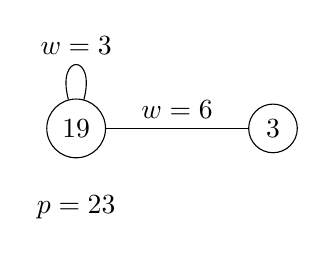
\begin{tikzpicture}

\node at (3,-1.5) { $p=23$};
  \node (A) at (3,-0.5) [circle,draw] {$19$};
  \node (B) at (5.5,-0.5) [circle,draw] {$3$};

  \draw (A) -- node[above] {$w=6$} (B);
  \draw (A) to [loop above] node {$w=3$} ();
  
\end{tikzpicture}
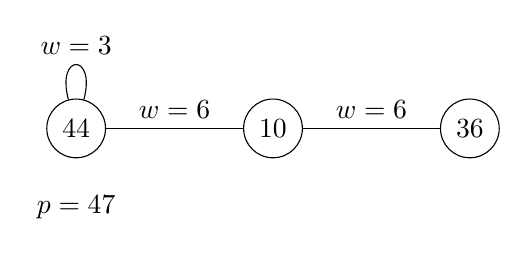
\begin{tikzpicture}
\node at (3,-1.5) { $p=47$};
  \node (A) at (3,-0.5) [circle,draw] {$44$};
  \node (B) at (5.5,-0.5) [circle,draw] {$10$};
\node (C) at (8,-0.5) [circle,draw] {$36$};

  \draw (A) -- node[above] {$w=6$} (B);
   \draw (B) -- node[above] {$w=6$} (C);
  \draw (A) to [loop above] node {$w=3$} ();
  
\end{tikzpicture}
\end{exam}
We show some properties of the graphs. 
\begin{lem}\label{propertiesofgraph}
Let $p>11$ be a prime. Then the graph $G_p$ has the following properties. 
    \begin{enumerate}
    
    \item [\rm{(a)}] All vertices other than those corresponding to $54000 \bmod p $ or $1728 \bmod p $ have degree $2$. 
        \item[\rm{(b)}] A vertex corresponding to $54000 \bmod p $ is the only vertex having a self loop. In addition, it is connected to another vertex by a single edge.
        \item [\rm{(c)}] A vertex corresponding to $1728 \bmod p $ is the only vertex having degree $1$. %必ずs.singになることもここで言っておいてね
           \item [\rm{(d)}] 
           
           Assume that there is an edge jointing vertices $x_1$ and $x_2$ and that a $\mu \in\fp$ satisfies $\{x_1,x_2\}=\{j(E_{\Lm^{-}(\mu)}),j(E_{\Lm^{+}(\mu)})\}$. Then the weight of the edge is $\#[\mu]$ where $[\mu]$ is as in Lemma \ref{num_iso}. More precisely, the weight of the self loop of the vertex $54000 \bmod p$ is $3$ and weights of all the other edges are $6$.
        
    \end{enumerate}
\end{lem}
\begin{proof}
(a) We start with a vertex $x_0$ that is not $54000 \bmod p $ or $1728 \bmod p $.  Since $x_0$ is the root of $P_p(X) \bmod p$, we may assume that an elliptic curve with $j$-invariant $x_0$ is defined by an equation $y^2=x(x-1)(x-t)$ with some $t\in \fp$.  By Lemma \ref{howmanylambda} and Lemma \ref{exactly2}, there are exactly two distinct $\fp$-elements $\lm_1,\lm_2$ and $\varepsilon_1,\varepsilon_2 \in \{\pm1\}$ such that $\Lm^{\varepsilon_1}(\lm_1)$ and $\Lm^{\varepsilon_2}(\lm_2)$ are equal to $t$.  Furthermore, from Lemma \ref{num_iso}, the set of $\fp$-elements $\lm$ that satisfy $j(E_{\Lm^{\varepsilon}(\lm)})=x_0$ with some $\varepsilon\in\{\pm1\}$ is $[\lm_1]\cup[\lm_2]$.  In addition, any element in $[\lm_1]$ (resp. $[\lm_2]$) gives the same edge from the vertex $x_0$. Our aim is to  show that the edges given by $[\lm_1]$ and $[\lm_2]$ are distinct, which occurs if and only if $\lm_2 \notin [\lm_1]$. Assume that $\lm_2\in [\lm_1]$. From Lemma \ref{num_iso}, the assumption that $\lm_2\in [\lm_1]$ and $\Lm^{\varepsilon_1}(\lm_1)=\Lm^{\varepsilon_2}(\lm_2)$ implies that $\Lm^{\varepsilon_1}(\lm_1)\in[1/2]$ or that $j\left(E_{\Lm^{-}(\lm_1)}\right)=j\left(E_{\Lm^{+}(\lm_1)}\right)$. The former case occurs only if $x_0\equiv1728\bmod p$. The latter case occurs only if $x_0\equiv54000 \bmod p$ from Proposition \ref{whenfp}. Thus, for vertices that do not correspond to $1728 \bmod p $ or $54000 \bmod p$, each of $[\lm_1]$ and $[\lm_2]$ gives distinct edge. Hence, the vertex $x_0$ has degree $2$.

(b) We note that the elliptic curve with $j$-invariant $54000\bmod p$ is supersingular when $p \equiv 11 \bmod 12$.  We know that $j(E_{\Lm^{-}(\lm)})\equiv j(E_{\Lm^{+}(\lm)})\equiv54000$ for $\lm\in[2]$ from Proposition \ref{whenfp}, so the vertex corresponding to $54000 \bmod p$ has a self loop. Proposition \ref{whenfp} also tells us that no other vertex has a self loop. In addition, from Lemma \ref{exactly2}, we have the other $\fp$-element $\mu\ne2$ such that $\Lm^{-}(\mu)=\Lm^{-}(2)$ or $\Lm^{+}(\mu)=\Lm^{-}(2)$. In order to show that $[2]$ and $[\mu]$ give distinct edges, it suffices to show that $\mu\notin [2]$. A direct calculation shows that $\Lm^{\pm}(1/2)=(2\pm\sqrt{3})/4$ and $\Lm^{\pm}(-1)=4(2\mp\sqrt{3})$ and then we see that they do not belong to $\{\Lm^{-}(2),\Lm^{+}(2)\}=\{-7\pm4\sqrt{3}\}$ for $p\ne 11$. Thus $\mu \notin[2]$.


(c)
We note that the elliptic curve $E$ with $j$-invariant $1728 \bmod p$ is supersingular when $p\equiv 11 \bmod 12$ and it can be given by the Legendre equation $y^2=x(x-1)(x+1)$. From Lemma \ref{exactly2}, we have exactly two $\fp$-elements $\lm_1,\lm_2$ such that $\Lm^{-}(\lm_i)$ or $\Lm^{+}(\lm_i)$ is equal to $1$ for $i=1,2$. The vertex $1728 \bmod p$ has only one edge if and only if $\lm_1$ and $\lm_2$ give the same edge, which occurs precisely when $\lm_1\in[\lm_2]$. We determine $\lm_1$ and $\lm_2$ explicitly from the $3$-torsion point of $E$ using Lemma \ref{exactly2}. The $x$-coordinate of $3$-torsion points are the roots of the following division polynomial of level $3$ of $E$:
\[
3x^4-6x^2-1=3\left(x^2-\frac{3+2\sqrt{3}}{3}\right)\left(x^2-\frac{3-2\sqrt{3}}{3}\right)=0.
\]
We note that $\pm\sqrt{3} \in \fp$ when $p \equiv11 \bmod 12$ and we see that
\[
\left( \frac{(3+2\sqrt{3})}{p} \right)\left( \frac{(3-2\sqrt{3})}{p} \right)=\left( \frac{-3}{p} \right)=-1.
\]
This means that either
$(3+2\sqrt{3})/3$ or $(3-2\sqrt{3})/3$ is quadratic mod $p$ and then we find that the division polynomial has exactly two $\fp$-roots. Let $\pm a$ be the two $\fp$-roots of the division polynomial. Using Lemma \ref{exactly2}, two $\fp$-elements $\lm_1$ and $\lm_2$ are written as follows:
\begin{align*}
    \lm_1:=\frac{f(a,a(a-1)(a+1))}{g(a,a(a-1)(a+1))}, \quad \lm_2=\frac{f(-a,-a(a-1)(a+1))}{g(-a,-a(a-1)(a+1))}.
\end{align*}
We set
\begin{align*}
   && f_1(a):=f(a,a(a-1)(a+1)), \quad f_2(a):=f(-a,-a(a-1)(a+1)),\\
   && g_1(a):=g(a,a(a-1)(a+1)), \quad g_2(a):=g(-a,-a(a-1)(a+1)) .
\end{align*}
Then a direct calculation shows that (see \cite[17]{Github})
\[
f_1g_2-f_1f_2+g_1f_2=0,
\]
which suggests that $\lm_1=\lm_2/(\lm_2-1)\in[\lm_2]$. This completes the proof.


(d) The first part of the lemma directly follows from Lemma \ref{num_iso}. In addition, since $\mu^2-\mu+1\ne 0$, $\#[\mu]=6$ for $\mu \notin [2]$ and $\#[\mu]=3$ for $\mu \in [2]$. From (b) we see that $\mu\in [2]$ corresponds to the self loop of the vertex $54000 \bmod p$. 
\end{proof} 
Now we are ready to prove Theorem \ref{thm:A} in the case of $p \equiv11 \bmod12$.
\begin{proof}[Proof of Theorem \ref{thm:A} in the case of $p \equiv11 \bmod12$] 
Firstly, we observe the case $p>11$.
    In order to determine the value of $\psi_p$, by Proposition \ref{arigataya}, we count the number of $\lm \in \fp$ such that the two elliptic curves $E_{\Lm^{-}(\lm)}$ and $E_{\Lm^{+}(\lm)}$ are supersingular. By Theorem \ref{important}, those $\lm\in \fp$ are exactly the $\lm\in \fp$ such that the $j$-invariants $j(E_{\Lm^{-}(\lm)})$ and  $j(E_{\Lm^{+}(\lm)})$ are the roots of $P_{p}(X) \bmod p$. Furthermore, it is exactly equal to the summation of the weights of all edges of the graph $G_p$. Since $1728 \not \equiv54000 \bmod p$ for $p>11$ and from lemma \ref{propertiesofgraph}, we obtain the following equation:
    \[
    \psi_p=\sum_{e\in E}w(e)=6(n-1)+3=6n-3
    \]
    where $n$ is the number of distinct roots of $P_p(X) \bmod p$.
   % \begin{tikzpicture}
  %\node (A) at (0,0) [circle,draw,inner sep=2pt] {$1728$};
  %\node (B) at (3,0) [circle,draw,inner sep=2pt] {$j_1$};
  %\node (C) at (8.2,0) [circle,draw,inner sep=2pt] {$54000$};
 % \node (D) at (5.2,0) [circle,draw,inner sep=2pt] {$j_2$};
 % \node at (1.5,0) { $\cdots$};
  %\node at (6.7,0) { $\cdots$};
  %\draw (A) -- node[above] {$3$} (1,0);
  %\draw (B) -- node[above] {$3$} (2,0);
  %\draw (B) -- node[above] {$3$} (4,0);
  %\draw (D) -- node[above] {$3$} (4.2,0);
  %\draw (D) -- node[above] {$3$} (6.2,0);
  %\draw (D) -- node[above] {$3$} (6.2,0);
 % \node at (4.5,0) { $\cdots$};
   %\draw (C) -- node[above] {$3$} (7.2,0);
   %\draw (C) to [loop below] node {3} ();
%\end{tikzpicture}
On the other hands, from Proposition \ref{fac_P_p}, the class number $h(-p)$ is written as follows:
\[
h(-p)=2(n-1)+1=2n-1.
\]
Hence we obtain for $p>11$
\[
\psi_p=3h(-p).
\]
Finally, for $p=11$ it is easy to see that $\psi_p=3h(-p)=3$.  
\end{proof}


\section{Proof of Theorem \ref{thm:B}}
\label{pfofb}
We prove Theorem \ref{thm:B} in \textcolor{black}{the introduction}. We use the idea by Fouvry and Murty \cite[Theorem 4]{FM01}. 

Let $X$, $\epsilon$ and $N$ be as in Theorem B. Theorem \ref{thm:A} enables us to write the summations $\sum_{|\lm| \le N} {\phi}_{\lm}(X)$ with the class numbers as follows. 
\begin{eqnarray}
    \sum_{|\lm| \le N} {\phi}_{\lm}(X) &=&  \sum_{|\lm| \le N} \sum_{\substack{p < X \\  C_{\lm} \text{ is superspecial} }} 1 
= \sum_{p < X} \sum_{\substack{|\lm| \le N \\ C_{\lm} \text{ is superspecial} }} 1 \nonumber\\
&=& \sum_{p < X}   \left( \frac{2N}{p} +O(1)  \right) {\psi}_{p} \nonumber\\
 &=& \!\!\! \sum_{\substack{p<X \\ p \equiv 1 \bmod 4}} \frac{2N}{p} \cdot \frac{3}{2} h(-3p) + \!\!\!  \sum_{\substack{p<X \\ p  \equiv 11 \bmod 12}} \frac{2N}{p}\cdot 3 h(-p)  +  O \left( X^{\frac{3}{2}} \right) .\nonumber\\&&\label{anaeq1}
%    \stepcounter{equation}\tag{\theequation}
\end{eqnarray}
%\begin{align*}
%\label{anaeq1}
%    \sum_{|\lm| \le N} {\phi}_{\lm}(X) &=&  \sum_{|\lm| \le N} \sum_{\substack{p < X \\  C_{\lm} \text{ is superspecial} }} 1 
%= \sum_{p < X} \sum_{\substack{|\lm| \le N \\ C_{\lm} \text{ is superspecial} }} 1 \\
%&=& \sum_{p < X}   \left( \frac{2N}{p} +O(1)  \right) {\psi}_{p} \\
% &=& \!\!\! \sum_{\substack{p<X \\ p \equiv 1 \bmod 4}} \frac{2N}{p} \cdot \frac{3}{2} h(-3p) + \!\!\!  \sum_{\substack{p<X \\ p  \equiv 11 \bmod 12}} \frac{2N}{p}\cdot 3 h(-p)  +  O \left( X^{\frac{3}{2}} \right) .
%    \stepcounter{equation}\tag{\theequation}
%\end{align*}
%&-& \sum_{\substack{p<X \\ p \equiv 3 \bmod 4}} \frac{4N}{p} + \sum_{\substack{p<X \\ p \equiv 1 \bmod 4}} h(-4p) \cdot r(p) + 6\sum_{\substack{p<X \\ p \equiv 3 \bmod 8}} h(-p) \cdot r(p)\\
%&+& 2\sum_{\substack{p<X \\ p \equiv 7 \bmod 8}} h(-p) \cdot r(p) - \sum_{\substack{p<X \\ p \equiv 3 \bmod 4 }}2r(p)+\sum_{p<X}2r'(p)
%+O(N),
We note that the sum of $h(-p)$ and $h(-3p)$ over primes less than $X$ is $O(X^{3/2})$.
(cf. Mertens \cite{FM} and  Siegel \cite{SI}). 
Recall the Dirichlet class number formula
\[
h(d)=\frac{\sqrt{|d|}}{ \pi}L(1,{\chi}_{d}),
\]
where $\chi_d$ is the character defined by the Kronecker symbol $(-d\ |\ \cdot)$.
%into equation \eqref{anaeq1},
Then the sum \eqref{anaeq1} is  
\begin{align*}
\label{anaeq2}
% & & \sum_{\substack{p<X\\ p \bmod 4=1}} \frac{2N}{p} h(-4p) + 6\sum_{\substack{p<X \\ p  \bmod 8=3}} \frac{2N}{p} h(-p) + 2\sum_{\substack{p<X \\ p \bmod 8=7}} \frac{2N}{p} \ h(-p) +o \left( \frac{N\sqrt{X}}{\log X} \right)\\
 % &=&\frac{2N}{\pi} \cdot 2 \sum_{\substack{p<X \\ \bmod 4=1}}\frac{1}{\sqrt{p}}L(1,{\chi}_{-4p})+ \frac{2N}{\pi} \cdot 6 \sum_{\substack{p<X \\ p \bmod 8 =3}}\frac{1}{\sqrt{p}}L(1,{\chi}_{-p})\\
  %&+&\frac{2N}{\pi} \cdot 2\sum_{\substack{p<X \\ p \bmod 8 =7}}\frac{1}{\sqrt{p}}L(1,{\chi}_{-p})+o \left( \frac{N\sqrt{X}}{\log X} \right) \\ 
  && \frac{2N}{\pi} \left(  \frac{3}{2}\sum_{\substack{p<X \\ p \equiv 1 \bmod 4}}\!\! \!\! \frac{\sqrt{3}}{\sqrt{p}}L(1,{\chi}_{-3p})+ \!\! \!\! \!\! \sum_{\substack{p<X \\ p \equiv 11\bmod 12 }} \!\! \!\!  \frac{3}{\sqrt{p}}L(1,{\chi}_{-p}) \right) + o \left( \frac{N\sqrt{X}}{\log X} \right).
  \stepcounter{equation}\tag{\theequation} 
\end{align*}
From Polya's inequality (cf. Apostol \cite[Theorem 8.21]{Apo}) and Abel's identity (cf. Apostol \cite[Theorem 4.2]{Apo}), for any parameter $U >1$, we have 
     \[
    \left| \sum_{U< n } \frac{{\chi}_{-p} (n)}{n} \right| < \frac{3\sqrt{p}\log p}{U}
    \]
    and the same inequality for $-3p$. 
%Hence we have
%\begin{eqnarray}
%\label{polyabel}
 %    \left| r_2(U,-p) \right| < \frac{3\sqrt{p}\log p}{U}, \quad \left| r_2(U,-4p)\right| < \frac{3\sqrt{4p}\log 4p}{U},
%\end{eqnarray}
%where 
%\begin{eqnarray*}
%    r_2(U,-p)=L(1,{\chi}_{-p})- \sum_{n \le U}\frac{{\chi}_{-p}(n)}{n},\\
 %   r_2(U,-4p)=L(1,{\chi}_{-4p})- \sum_{n \le U}\frac{{\chi}_{-4p}(n)}{n}.
%\end{eqnarray*}
We choose $U=X^{3/4}$. Then \eqref{anaeq2} is as follow\textcolor{black}{s}.
\begin{align*}
\label{anaeq3}
   \frac{6N}{\pi} \left\{ \frac{\sqrt{3}}{2} \!\!\!\sum_{\substack{p<X \\ p \equiv 1 \bmod 4}}\!\!\!\!\frac{1}{\sqrt{p}} \sum_{n \le U}\frac{{\chi}_{-3p}(n)}{n}+  \!\!\!\!\!\!\sum_{\substack{p<X \\ p \equiv 11 \bmod 12 }} \!\!\!\!\frac{1}{\sqrt{p}}\sum_{n \le U} \frac{{\chi}_{-p}(n)}{n} \right\}
    + o \left( \frac{N\sqrt{X}}{\log X} \right)
     \stepcounter{equation}\tag{\theequation} .
\end{align*}

%\begin{rem}
%Using the inequalities \eqref{polyabel}, 
%we see that the error terms from $r_2(U,-p)$ and %$r_2(U,-4p)$ are smaller than 
%\[
%C \cdot N \sum_{p < X} \frac{\log 4p}{U}
%\]
%for a certain constant $C$. Since $U=X^{3/4}$, we %see that the error terms are ultimately negligible compared to $N\sqrt{X}/ \log X$.
    %\begin{eqnarray*}
     %  &&  \frac{2N}{\pi} \Biggr| 2 \sum_{\substack{p<X \\ p \bmod 4=1}}\frac{1}{\sqrt{p}} \cdot r_2(U,-4p) + 6\sum_{\substack{p<X \\ p \bmod 8 =3}}\frac{1}{\sqrt{p}} \cdot r_2(U,-p)\\   
      %  &+& 2\sum_{\substack{p<X \\ p \bmod 8 =7}}\frac{1}{\sqrt{p}} \cdot r_2(U,-p)  \Biggr|\\
       % &\le&\frac{2N}{\pi}\cdot \left( 2 \sum_{\substack{p<X \\ p \bmod 4=1}} \frac{ 6\log 4p}{U} +6 \sum_{\substack{p<X \\ p \bmod 8 =3}}\frac{3\log p}{U}  +   2\sum_{\substack{p<X \\ p \bmod 8 =7}} \frac{3\log p}{U} \right) \\
        %&\le&\frac{2N}{\pi} \cdot 6 \sum_{p < X} \frac{6\log 4p}{U} .
    %\end{eqnarray*}
    %Since
   % \begin{eqnarray*}
        %\sum_{p< X} \frac{\log 4p}{U}&=& \frac{1}{X^{\frac{3}{4}}}\sum_{p < X} \log 4p\le \frac{1}{X^{\frac{3}{4}}}\sum_{2 \le n < X} \log 4n \\ &\le & \frac{1}{X^{\frac{3}{4}}} \int_{2}^{X+1} \log4t \ dt = O(X^{\frac{1}{4}} \log X)= o\left( \frac{\sqrt{X}}{\log X} \right) ,
   % \end{eqnarray*}
    
   % the error term is $o(N\sqrt{X}/ \log X)$.
%\end{rem}
We recall that ${\chi}_{-3p}$ and ${\chi}_{-p}$ are expressed by the Legendre symbols: 
 if $p \equiv 1\bmod 4$\textcolor{black}{, then}
    \[
    {\chi}_{-3p}= \left( \frac{n}{3} \right) \left( \frac{n}{p} \right),
    \]
if $p \equiv 3 \bmod 4$\textcolor{black}{, then}
     \[
    {\chi}_{-p}= \left( \frac{n}{p} \right).
    \]
Substituting these \textcolor{black}{in} \eqref{anaeq3} yields
\begin{align*}
\label{anaeq4}
   && \frac{3\sqrt{3}N}{\pi}S(X,U) +  \frac{6N}{\pi} T(X,U)
    + o \left( \frac{N\sqrt{X}}{\log X} \right),
     \stepcounter{equation}\tag{\theequation} 
\end{align*}
where
\begin{eqnarray*}
    S(X,U)&:=& \sum_{n \le U} \frac{1}{n} \sum_{\substack{p<X \\ p \equiv1 \bmod 4}}\frac{\left( \frac{n}{3} \right) \left( \frac{n}{p} \right)}{\sqrt{p}},\\
    T(X,U)&:=&\sum_{n \le U} \frac{1}{n} \sum_{\substack{p<X \\ p \equiv 11\bmod 12}}\frac{\left( \frac{n}{p} \right)}{\sqrt{p}}.
\end{eqnarray*}
We calculate these sums using the idea of Fouvry and Murty \cite[Theorem 4]{FM01}.

We first calculate $T(X,U)$. If we sum over only $n \le U$ such that $n$ is a perfect square or $n/3$ is a perfect square, then we have 
    \begin{eqnarray*}
    \sum_{\substack{n \le U \\ n=d^2 \text{ for some } d \in \bN }} \frac{1}{d^2} \sum_{\substack{p<X \\ p \equiv 11 \bmod 12 }} \frac{1}{\sqrt{p}}+\sum_{\substack{n \le U \\ n=3l^2 \text{ for some } l \in \bN }} \frac{1}{3l^2} \sum_{\substack{p<X \\ p \equiv 11 \bmod 12}} \frac{1}{\sqrt{p}}.
    \end{eqnarray*}
we note that $3 \in {{\fp}^{*}}^2$ if $p \equiv 11 \bmod 12$. 
We know that the inner sum of each term is equal to
\[
\frac{2}{\varphi(12)} \frac{\sqrt{X}}{\log X} +o \left( \frac{\sqrt{X}}{\log X} \right),
\]
where $\varphi$ is Euler's totient function. 
Thus, we get
\[
 \sum_{\substack{n \le U \\ n=d^2 \text{ for some } d \in \bN }} \frac{1}{d^2} \sum_{\substack{p<X \\ p \equiv 11 \bmod 12 }} \frac{1}{\sqrt{p}}=\frac{{\pi}^2}{12} \frac{\sqrt{X}}{\log X} +o \left( \frac{\sqrt{X}}{\log X} \right)
\]
and
\[
\sum_{\substack{n \le U \\ n=3l^2 \text{ for some } l \in \bN }} \frac{1}{3l^2} \sum_{\substack{p<X \\ p \equiv 11 \bmod 12 }} \frac{1}{\sqrt{p}}=\frac{{\pi}^2}{36} \frac{\sqrt{X}}{\log X} +o \left( \frac{\sqrt{X}}{\log X} \right).
\]
\textcolor{black}{Following a similar approach to} Fouvry and Murty \cite[p.\ 92]{FM01} and using Lemma \ref{jutila}, the sum of the remaining terms is ultimately negligible compared to $\sqrt{X}/ \log X$.
Hence we obtain
\begin{eqnarray}
\label{11mod12}
    T(X,U)=\frac{{\pi}^2}{9} \frac{\sqrt{X}}{\log X} +o \left( \frac{\sqrt{X}}{\log X} \right).
\end{eqnarray}

Second, we calculate $S(X,U)$. If $3$ divides $n$, then ${\chi}_{-3p}(n)$ is $0$ so we only treat $n$ such that $3 \nmid n $. If we sum over only such $n \le U$  that is also perfect square, then we have
  \begin{eqnarray*}
   && \sum_{\substack{n \le U \\ n=d^2 \text{ for some } d \in \bN, \ 3 \nmid d}} \frac{1}{d^2} \sum_{\substack{p<X \\ p \equiv 1  \bmod 4}} \frac{1}{\sqrt{p}}\\ &&=\left(\sum_{\substack{n \le U \\ n=d^2 \text{ for some } d \in \bN}} \frac{1}{d^2} -\sum_{\substack{n \le U \\ n=(3d)^2 \text{ for some } d \in \bN}} \frac{1}{(3d)^2}\right)\sum_{\substack{p<X \\ p \equiv 1  \bmod 4}} \frac{1}{\sqrt{p}}.
    \end{eqnarray*}
    We know that 
    \begin{eqnarray*}
     && \sum_{\substack{p<X \\ p\equiv 1 \bmod 4}} \frac{1}{\sqrt{p}}=  \frac{2}{\varphi(4)} \frac{\sqrt{X}}{\log X} +o \left( \frac{\sqrt{X}}{\log X} \right).
    \end{eqnarray*}
    Thus we obtain 
    \begin{eqnarray*}
         \sum_{\substack{n \le U \\ n=d^2,\ \exists d \in \bN,\ 3 \nmid d }} \frac{1}{d^2} \sum_{\substack{p<X \\ p \equiv 1 \bmod 4 }} \frac{1}{\sqrt{p}}=\frac{{4\pi}^2}{27}\frac{\sqrt{X}}{\log X} +o \left( \frac{\sqrt{X}}{\log X} \right).
    \end{eqnarray*}
\textcolor{black}{Following a similar approach to} Fouvry and Murty \cite[p.92]{FM01}, the sum of the remaining terms is ultimately negligible compared to $\sqrt{X}/ \log X$.  Thus we find that
\begin{eqnarray}
\label{1mod4}
    S(X,U)=\frac{4{\pi}^2}{27}\frac{\sqrt{X}}{\log X} +o \left( \frac{\sqrt{X}}{\log X} \right).
\end{eqnarray}
Substituting the equations \eqref{11mod12}, \eqref{1mod4} for \eqref{anaeq4} yields 
\[
 \sum_{|\lm| \le N} {\phi}_{\lm}(X) =\frac{(6+4\sqrt{3})\pi N}{9}\frac{\sqrt{X}}{\log X} +o \left( \frac{N \sqrt{X}}{\log X} \right).
\]
Hence we obtain
\[
 \frac{1}{N}\sum_{|\lm| \le N} {\phi}_{\lm}(X) =\frac{(6+4\sqrt{3})\pi }{9} \frac{\sqrt{X}}{\log X} +o \left( \frac{ \sqrt{X}}{\log X} \right).
\]
\section{Proof of Theorem \ref{thm:C}}
\label{pfofc}
In this section, we prove Theorem \ref{thm:C}.  From our previous work \cite[\S 6]{Ando}, we have
\begin{eqnarray*}
    \sum_{\text{ht}(\lm) \le N} {\phi}_{\lm}(X) &=& 
\sum_{p < X} \sum_{\substack{\text{ht}(\lm) \le N \\ C_{\lm} \text{ is superspecial} }} 1\\
&=& \sum_{p < X} \left(  \frac{12}{{\pi}^2} \frac{N^2}{p} + o(N\log N) +O\left( \frac{N^2}{p^2} \right) \right) {\psi}_p.
\end{eqnarray*}
Thus, from the result of Theorem B we find that
\[
\sum_{\lm \in \bQ,\ \height(\lm) \le N } {\phi}_{\lm}(X) = \frac{4(3+2\sqrt{3})}{3\pi} \frac{N^2\sqrt{X}}{\log X} +o \left( \frac{N^2\sqrt{X}}{\log X}\right).
\]
Hence we obtain
 \[
    \frac{1}{N^2}\sum_{\lm \in \bQ,\ \height(\lm) \le N } {\phi}_{\lm}(X) = \frac{4(3+2\sqrt{3})}{3\pi} \frac{\sqrt{X}}{\log X} +o \left( \frac{\sqrt{X}}{\log X}\right).
 \]

\begin{comment}
\section{Appendix}
\label{appendix}
\subsection{A generalization of the Kronecker congruence relation}
We give a generalization of the Kronecker congruence relation on modular polynomials.

The modular polynomial $\Phi_n(X,Y)$ for level $n$
is a polynomial in $X$ and $Y$ characterized by
the condition that $\Phi_n(j(E_1),j(E_2))=0$
if and only if there exists an isogeny $E_1 \to E_2$
of elliptic curves whose kernel is a cyclic group of order $n$. It is known that $\Phi_n(X,Y) \in \Z[X,Y]$.
We briefly review more concrete construction of the polynomial.
Let $n$ be a natural number and consider
%\[
%\Delta_n := \{\alpha\in {\rm M}_2(\Z) \mid \det \alpha = n\}
%\]
%and
\[
\Delta_n^* := \left\{\left. \alpha=\begin{pmatrix}a & b\\
c & d\end{pmatrix}\in {\rm M}_n \ \right| \  \det \alpha = n,\ \gcd(a,b,c,d)=1\right\}.
\]
A complete system of representatives of $\SL_2(\Z)\backslash \Delta_n^*$ is given by
\[
\overline{\Delta}_n^*:=\left\{\left.
\begin{pmatrix}
a & b\\
0 & d
\end{pmatrix} \in \Delta_n^* \ \right| \ 
0 < a, \ 0 \leq b < d, \ ad =n
\right\}
\]
cf. \cite[5, \S~1]{SL}.
Let $j : {\mathbb H} \to \bC$ be the map associating
$\tau$ to $j(\tau)$, where $j(\tau)$ is the $j$-invariant of the elliptic curve $\bC/(\bZ + \bZ \tau)$.
The modular polynomial for level $n$ satisfies
\[
\Phi_n(X,j(\tau)) = \prod_{\alpha\in \overline{\Delta}_n^*} (X-j(\alpha z)),
\]
where $\alpha\tau = \frac{a\tau + b}{d}$ for $\alpha = \begin{pmatrix}a & b \\ 0 & d\end{pmatrix}$.
It is known that $\Phi_n(X,j) \in \Z[X,j]$.
The next proposition may be well-known but we write it for the convenience of the reader.
\begin{prop}
Let $p$ be a prime and $n$ an integer with $\gcd(n,p)=1$. We have
\[
\Phi_{pn}(X,j) \equiv \Phi_n(X,j^p)\Phi_n(X^p,j) \pmod p.
\]
The case of $n=1$ is called the Kronecker congruence relation (cf. \cite[5, \S 3, Theorem 5]{SL}).
\end{prop}
\begin{proof}
Consider the decomposition
\[
\overline{\Delta}_{p n}^* =
\Delta_+ \sqcup \Delta_-,
\]
where
\begin{eqnarray*}
\Delta_+ &:=&\left\{\left.
\begin{pmatrix}
a & b\\
0 & d
\end{pmatrix} \in \Delta_{pn}^* \ \right| \ 
p|a
\right\},\\
\Delta_- &:=&\left\{\left.
\begin{pmatrix}
a & b\\
0 & d
\end{pmatrix} \in \Delta_{pn}^* \ \right| \ 
p|d
\right\}.
\end{eqnarray*}

%\begin{eqnarray*}
%\Delta_{p,\ell} &:=& \left\{\left.
%\begin{pmatrix}
%p & b\\
%0 & \ell
%\end{pmatrix} \right|
%0 \leq b < \ell
%\right\}\\
%\Delta_{\ell,p} &=& \left\{\left.
%\begin{pmatrix}
%\ell & b\\
%0 & p
%\end{pmatrix} \right|
%0 \leq b < p
%\right\}\\
%\Delta_{p\ell,1} &=& \left\{
%\begin{pmatrix}
%p\ell & 0\\
%0 & 1
%\end{pmatrix} 
%\right\}\\
%\Delta_{1,p\ell} &=& \left\{\left.
%\begin{pmatrix}
%1 & b\\
%0 & p\ell
%\end{pmatrix} \right|
%0 \leq b < p\ell
%\right\}\\
%\end{eqnarray*}

With $q=e^{2\pi i \tau}$,
write
\[
j(\tau) = \frac{1}{q} + P(q)
\]
for a power series $P$ in $q$ with integer coefficients.
Since
$\alpha \tau = \frac{a\tau + b}{d}$, we have
\[
j(\alpha\tau) = \frac{1}{\zeta_d^b q^{a/d}} + P(\zeta_d^b q^{a/d}),
\]
where $\zeta_d = e^{2\pi i /d}$. 

For $\alpha = \begin{pmatrix}a & b \\ 0 & d\end{pmatrix}\in\Delta_+$, we set
$
\alpha' = \begin{pmatrix}a/p & b' \\ 0 & d\end{pmatrix}\in\overline{\Delta}_{n}^*
$ with $b\equiv pb' \pmod d$, 
%and for $\alpha = \begin{pmatrix}p\ell & 0 \\ 0 & 1\end{pmatrix}\in\Delta_{p\ell,1}$, we set
%$
%\alpha' = \begin{pmatrix}\ell & 0 \\ 0 & %1\end{pmatrix}\in\Delta_{\ell,1}
%$, 
we have
\[
j(\alpha \tau ) \equiv j(\alpha' \tau)^p \pmod p.
\]
For $\alpha = \begin{pmatrix}a & b \\ 0 & d\end{pmatrix}\in\Delta_-$, we set
$
\alpha' = \begin{pmatrix}a & b' \bmod d/p\\ 0 & d/p\end{pmatrix}\in\overline{\Delta}_{n}^*
$ with $\zeta_d^b = (\zeta_p\zeta_{d/p})^{b'}$, 
%and for $\alpha = \begin{pmatrix}p\ell & 0 \\ 0 & 1\end{pmatrix}\in\Delta_{p\ell,1}$, we set
%$
%\alpha' = \begin{pmatrix}\ell & 0 \\ 0 & %1\end{pmatrix}\in\Delta_{\ell,1}
%$, 
we have
\[
j(\alpha \tau ) \equiv j(\alpha' \tau)^{1/p} \quad \bmod {(1-\zeta_p)\Z[\zeta_{pn}]}.
\]

From these, we obtain
\[
\Phi_{pn}(X,j) \equiv \Phi_n(X,j^p)\Phi_n(X^p,j) \quad \bmod {(1-\zeta_p)\Z[\zeta_{pn}]}.
\]
The proposition follows from the fact that
the both sides are elements of $\Z[X,j]$.
\end{proof}
\end{comment}
 
\subsection*{Data availability statement} 
Data sharing is not applicable to this article, as no datasets were generated or analyzed during the present work.

\subsection*{Conflict of interest}
The authors declare no conflicts of interest associated with this manuscript.
\begin{thebibliography}{99}
\bibitem{AT02}
R.\ Auer and J.\ Top:
\textit{Legendre elliptic curves over finite fields.}
J.\ Number Theory {\bf 95},\ No.\ 2,\ 303--312 (2002)

\bibitem{Apo}
T.\ M.\ Apostol: \textit{Introduction to Analytic Number Theory.}
Springer-Verlag,\ 1976.

\bibitem{Ando}
C. Ando:
\textit{The Lang-Trotter conjecture on average for genus-$2$ curves with Klein-$4$ reduced automorphism group.}
Res. number theory {\bf 11}, 83 (2025).

\bibitem{SB}
S. Baier:
\textit{The Lang-Trotter conjecture on average.}
J. Ramanujan Math. Soc. {\bf 22}. No. 4, 299--314 (2007)

\bibitem{Magma}
W.\ Bosma, J.\ Cannon, C.\ Playoust: \textit{The Magma algebra system. I. The user language}, Journal of Symbolic Computation {\bf 24}, 235--265  (1997). %DOI: 10.1006/jsco.1996.0125

%\bibitem{MagmaHP}
%Cannon, J., et al. (2016). Magma A Computer Algebra System,
%School of Mathematics and Statistics, University of Sydney, 2016.\ %\texttt{http://magma.maths.usyd.edu.au/magma/}


\bibitem{DP}
C.\ David and F.\ Pappalardi:
\textit{Average frobenius distribution of elliptic curves}
\textcolor{black}{
Int.\ Math.\ Res.\ Not.\ (1999) 165--183.}

\bibitem{Deu}
M.\ Deuring:
\textit{Die typen der multiplikatorenringe elliptischer funktionenk\"{o}rper.}
Abh.\ Math.\ Sem.\ Univ.\ Hamburg  {\bf 14}, 197--272 (1941) 

\bibitem{Dorman}
D.\ R.\ Dorman:
\textit{Special values of the elliptic modular function and factorization formulae.}
J.\ Reine Angew.\ Math.\ {\bf 383} (1988), 207--220.

\bibitem{Elkies}
N.\ D.\ Elkies: 
\textit{The existence of infinitely many supersingular primes for every elliptic curve over $\mathbb Q$.} 
Invent. Math. {\bf 89}, No.\ 3 561--567 (1987)


\bibitem{FM01}
E.\ Fouvry and M.\ R.\ Murty:
\textit{On the distribution of supersingular primes.}
Can.\ J.\ Math.\ {\bf 48},\ No.\ 1,\ 81--104 (1996)

\bibitem{GZ}
B.\ Gross and D.\ Zagier:
{\it On singular moduli.}
%(English) Zbl 0545.10015
J. Reine Angew. Math. {\bf 355}, 191--220 (1985).


 \bibitem{IKO02}
 T.\ Ibukiyama, T.\ Katsura, and F.\ Oort:
 \textit{Supersingular curves of genus two and class numbers.}
 Compos.\  Math.\ {\bf 57},\ No.\ 2,\ 127--152 (1986)

 \bibitem{IKadd}
 T.\ Ibukiyama and T.\ Katsura:
 \textit{On the field of definition of superspecial
polarized abelian varieties and type numbers.}
Compos.\ Math.\  {\bf 91}, (1994), 37-46.
\bibitem{Igusa_ell}
J.\ Igusa: \textit{Kroneckerian model of fields of elliptic modular functions.}
Am.\ J.\ Math.\ {\bf 81}, \ 561--577 (1959)


\bibitem{Igusa}
J.\ Igusa:
\textit{Arithmetic variety of moduli for genus two.}
Ann. of Math. {\bf 72}, No.3, 612--649 (1960)

\bibitem{Ju}
M.\ Jutila:
\textit{On the meaning value of $L(\frac{1}{2}, \chi)$.}
Analysis {\bf 1} (1981) 149--161 

\bibitem{KatsuraOort}
T.\ Katsura and F.\ Oort:
\textit{Supersingular abelian varieties of dimension two or three and class numbers.}
Algebraic geometry,\ Proc.\ Symp.\  Sendai,\ 1985,\ Adv.\ Stud.\ Pure Math.\ {\bf 10}, 253-281 (1987).
\bibitem{kaneko}
M. Kaneko:
\textit{Supersingular $j$-invariants as singular moduli mod $p$.}
Osaka\ J.\  Math.\ {\bf 26}, No.\ 4,\ 849--855 (1989) 


\bibitem{LT}
S.\ Lang and H.\ Trotter:
\textit{Frobenius distributions in ${GL}_2$-extensions.}
%\textit{Frobenius in ${GL}_2$ extensions.}
Lecture Notes in Math. {\bf 504}, Springer-Verlag, Berlin (1976)

\bibitem{SL}
S. Lang: \textit{Elliptic Functions.
2nd edition.} Graduate Texts in Mathematics, {\bf 112}, Springer-Verlag, New York, 1987


%\bibitem{M1319}
%P.\ Manfred:
%\textit{The distribution of class numbers of pure number fields(Diophantine problems and analytic number theory).}
%RIMS Kôkyûroku published {\bf 1319} 193--197 (2003)

\bibitem{FM}
F.\ Mertens:
\textit{\"{U}ber einige asymptotische Gesetze der Zahlentheorie.} 
J. Reine Angew. Math. {\bf 77} (1874) 289-338

\bibitem{SI}
C.\ L.\ Siegel:
\textit{The average measure of quadratic forms with given determinant and signature.}
Ann. of Math. { \bf 45} (1944) 667--68

\bibitem{AEC}
J.\ H.\ Silverman:
\textit{The Arithmetic of Elliptic Curves. 2nd edition.}
Graduate Texts in Mathematics {\bf 106}, Springer  2010.


%\bibitem{Yui}
%N.\ Yui:
%\textit{On the Jacobian varieties of hyperelliptic curves over fields of characteristic $p > 2$.}
%Journal of Algebra {\bf 52},\ No.\ 2,\ 378--410 (1978)

\bibitem{Top}
J.\ Top: \textit{Descent by 3-isogeny and 3-rank of quadratic fields.} 
Advances in Number Theory: The
Proceedings of the Third Conference of the Canadian Number Theory Association (1993),
303--317.
%Advances in number
% theory, (1993) 303--317.

\bibitem{Github}
GitHub repository: Codes$\_$for$\_$the$\_$LT$\_$conjecture$\_$on$\_$average$\_$for$\_$genus2\\$\_$curves$\_$with$\_$S3$\_$reducedautomorphism$\_$group\\
\url{https://github.com/tremolopluschihiro/Codes_for_the_LT_conjecture_on_average_for_genus2_curves_with_S3_reducedautomorphism_group}
\begin{enumerate}
\item[] \texttt{1\_lemma\_3.1.m}
\item[] \texttt{2-1$\_$lemma\_3.2.m}
\item[] \texttt{2-2$\_$lemma$\_$3.2.m}
\item[] \texttt{3-1$\_$lemma$\_$3.2.m}
\item[] \texttt{3-2$\_$lemma$\_$3.2.m}
\item[] \texttt{4-1$\_$proposition$\_$3.3.m}
\item[] \texttt{4-2$\_$proposition$\_$3.3.m}
\item[] \texttt{5-1$\_$remark$\_$3.6.m}
\item[] \texttt{5-2$\_$remark$\_$3.6.m}
\item[] \texttt{5-3$\_$remark$\_$3.6.m}
\item[] \texttt{6-1$\_$proposition$\_$5.4.m}
\item[] \texttt{6-2$\_$proposition$\_$5.4.m}
\item[] \texttt{7$\_$theorem$\_$6.2.m}
\item[] \texttt{8$\_$lemma$\_$6.3.m}
\item[] \texttt{9-1$\_$lemma$\_$6.6.m}
\item[] \texttt{9-2$\_$lemma$\_$6.6.m}
\item[] \texttt{10$\_$lemma$\_$7.4.m}
\item[] \texttt{11$\_$proposition$\_$7.5.m}
\item[] \texttt{12$\_$proposition$\_$7.5.m}
\item[] \texttt{13$\_$proposition$\_$7.5.m}
\item[] \texttt{14$\_$proposition$\_$7.7.m}
\item[] \texttt{15$\_$proposition\_7.7\_(d).m}
\item[] \texttt{16$\_$lemma\_7.8.m}
\item[] \texttt{17$\_$lemma\_8.2\_(c).m}
\end{enumerate}
\end{thebibliography}


\end{document}
